% !TEX root = ejemplo-memoria.tex

\documentclass[twoside,spanish,a4paper,12pt]{tfg}

% Editar la titulación
\titulacion{Grado en Ingeniería Multimedia}

% Editar el título
\title{DONA’m MÓN: Aplicación móvil para visibilizar la vida y obra de mujeres en puntos geolocalizados de Valencia.}

% Si es una alumna se debe usar
% \authorlabel{Autora}
\authorlabel{Autor}
% Editar el nombre
\author{Ivana Stanislavova Ivanova}


% Si hay varios tutores:
% \tutorlabel{Tutores}
% \tutor{Nombre del tutor 1 \\[2mm] Nombre del turor2}
\tutorlabel{Tutor}
% Editar
\tutor{Manuel Pérez Aixendri}

% Editar: Poner mes y año de la convocatoria de lectura del TFM
\convocatoria{Enero 2025}

\usepackage{float}
\usepackage[table]{xcolor}
\usepackage{tabularx}
\usepackage{graphicx}
\usepackage{amsmath}
\usepackage{amssymb}
\usepackage{amsfonts}
\usepackage{titlesec}
\usepackage{eurosym}
\usepackage{pgfgantt}
\usepackage{pdflscape}
\usepackage[utf8]{inputenc}
\titlespacing*{\section}{0pt}{1.9ex plus 0.8ex minus .2ex}{1.2ex}
\titlespacing*{\subsection}{0pt}{.4ex plus 0.6ex minus .2ex}{0.9ex}

% Corregir error de headheight para fancyhdr
\setlength{\headheight}{14.5pt}

\begin{document}

% NO QUITAR ESTOS ELEMENTOS
\portada
\cleardoublepage
\contraportada
\cleardoublepage
\declaracion
\cleardoublepage


% Editar: Resumen en Español (obligatorio)
\begin{resumen}
  Este es el resumen del TFM. Debe ser corto (máximo media página) y cubrir los aspectos principales del TFM.
\end{resumen}
\cleardoublepage

% Editar: Resumen en Inglés
\begin{abstract}
  This is the abstract of the TFM. It must be short and cover the main aspects of the TFM.
\end{abstract}
\cleardoublepage

% Editar: Resumen en Valenciano
\begin{resum}
  Aquest és el resum del TFM. Ha de ser curt (màxim mitja pàgina) i cobrir els aspectes principals del TFM.
\end{resum}
\cleardoublepage


% Editar: Agradecimientos (opcional)
\begin{agradecimientos}

\end{agradecimientos}
\cleardoublepage

\tableofcontents

\pagestyle{tfg}
\justify

% Las figuras se buscan en el directorio figs

% Cada capítulo está en su propio fichero tex. Ver el directorio tex.

% La bibliografía está dentro del directorio bib
\chapter{Introducción}
% !TEX root = ../ejemplo-memoria.tex
% Contenidos del capítulo.
% Las secciones presentadas son orientativas y no representan
% necesariamente la organización que debe tener este capítulo.

\section{Introducción}


En la actualidad, la tecnología se ha convertido en una herramienta clave para trans-
formar la forma en la que interactuamos con nuestro entorno, permitiendo nuevas maneras
de aprender, explorar y conectarnos con la historia y la cultura. Sin embargo, la construcción de los relatos históricos y culturales ha tendido a otorgar mayor protagonismo a figuras masculinas, dejando en la sombra numerosas contribuciones femeninas de gran relevancia en ámbitos como la ciencia, el arte, la política o la educación.

Este Trabajo de Fin de Grado se centra en el desarrollo de una aplicación móvil interactiva basada en geolocalización y realidad aumentada (RA), que tiene como objetivo visibilizar el legado de mujeres con relevancia histórica que han nacido, vivido, desarrollado parte de su labor o tenido relevancia en Valencia. Mediante esta aplicación, los usuarios podrán desbloquear contenido educativo y multimedia al visitar puntos de interés geolocalizados, conectando los lugares emblemáticos de la ciudad con las historias de estas mujeres, conociendo su vida y obra.

La aplicación lleva por nombre DONA’m MÓN, una frase en valenciano con doble significado en su primera palabra: “dona” puede leerse tanto como sustantivo (“mujer”) o como forma verbal (“dame”).  Así que el título leído como “Dame mundo”, esconde un juego de palabras que representa el propósito del proyecto: ofrecer a las mujeres este espacio real y simbólico en el mundo, un lugar en el mapa donde su historia pueda ser descubierta y reconocida.

DONA’m MÓN ofrece una experiencia educativa y lúdica que invita a reflexionar sobre la igualdad de género. Este proyecto pretende ser un puente entre el pasado y el presente, ayudando a los usuarios a redescubrir la ciudad desde esta nueva perspectiva inclusiva.



\section{Motivación}
El desarrollo de este proyecto surge de una doble motivación: por un lado, mi interés personal en el desarrollo de tecnologías con un propósito educativo y social, y por otro, el deseo de poner en valor las aportaciones de las mujeres a lo largo de la historia.

Durante mi recorrido académico como estudiante de Ingeniería Multimedia y en mi máster actual en Tecnologías web, Aplicaciones móviles y Computación en la nube, he desarrollado un fuerte interés por aplicar el conocimiento técnico en proyectos que tengan un impacto positivo en la sociedad, orientados a transformar la manera en la que accedemos y transmitimos el conocimiento.

Además, como mujer en STEM, considero importante que este proyecto consiga ayudar en la visibilización del papel femenino en todas las áreas del saber y a toda clase de público. Aunque se han producido avances significativos en materia de igualdad, los datos actuales evidencian que la brecha persiste: solo el 33\% de los investigadores a nivel mundial son mujeres, y en campos como la inteligencia artificial esta cifra desciende al 22\%~\cite{unesco2021}. En el contexto español, apenas el 24\% de las cátedras universitarias están ocupadas por mujeres, según el informe “Científicas en Cifras 2021” del Ministerio de Ciencia e Innovación~\cite{cientificas2021}. Estas cifras reflejan una infrarrepresentación que no solo afecta a la ciencia, sino también a otros ámbitos clave del desarrollo cultural y social.

Valencia, como muchas otras ciudades, alberga una historia rica y compleja en la que también han participado numerosas mujeres valiosas, desde científicas y artistas hasta activistas y educadoras. Muchas de ellas siguen siendo poco conocidas fuera de círculos especializados. Este proyecto representa una oportunidad para darles mayor protagonismo, aprovechando tecnologías como la realidad aumentada y la geolocalización para generar experiencias de aprendizaje activas, accesibles e innovadoras.

Por todo esto, el objetivo de este trabajo no es solo técnico, sino también ético y cultural: contribuir, desde la tecnología, a construir una memoria más justa e inclusiva.

\section{Objetivos}
El objetivo principal de este proyecto es desarrollar una aplicación móvil interactiva que utilice tecnologías de geolocalización, realidad aumentada (RA) y una base de datos centralizada para visibilizar y divulgar las historias de mujeres destacadas en la ciudad de Valencia, promoviendo su reconocimiento histórico y cultural a través de una experiencia inmersiva, educativa y accesible para los usuarios.

Descomponiendo este objetivo principal, se definen los siguientes objetivos específicos:

\begin{itemize}
    \item \textbf{Investigación y selección de mujeres invisibilizadas:}
    \begin{itemize}
        \item Identificar figuras femeninas históricas relacionadas con Valencia que hayan destacado en campos como la ciencia, el arte, la política o los derechos sociales.
        \item Asociar a cada figura un punto geolocalizado en la ciudad con un vínculo significativo con su historia.
    \end{itemize}

    \item \textbf{Creación y gestión de una base de datos con MySQL:}
    \begin{itemize}
        \item Diseñar y desarrollar una base de datos relacional en MySQL, estructurada para almacenar de forma eficiente información sobre las mujeres seleccionadas, sus ubicaciones geográficas y el contenido multimedia vinculado.
        \item Implementar un backend utilizando el framework Django, asegurando la integridad, consistencia y seguridad de los datos mediante su ORM, y exponiendo una API RESTful que permita su acceso y manipulación desde la aplicación móvil.
    \end{itemize}


    \item \textbf{Desarrollo de funcionalidades tecnológicas:}
    \begin{itemize}
        \item Implementar un sistema de geolocalización que permita a los usuarios desbloquear contenido interactivo al acercarse a los puntos de interés.
        \item Integrar elementos de realidad aumentada desarrollados con A-Frame, que permitan visualizar objetos, imágenes o recreaciones 3D relacionadas con las mujeres seleccionadas al enfocar con la cámara del dispositivo móvil.
        \item Implementar un sistema de notificaciones que alerte a los usuarios al aproximarse a un punto de interés relevante, mejorando la interacción con el entorno urbano y fomentando la exploración activa.
    \end{itemize}

    \item \textbf{Diseño de una experiencia de usuario intuitiva y atractiva:}
    \begin{itemize}
        \item Crear una interfaz accesible y adaptada al entorno móvil con React Native y Expo Go, que facilite la navegación y el uso de las funcionalidades principales de la aplicación.
        \item Incluir un mapa interactivo con los puntos de interés marcados, accesibles según la ubicación del usuario.
    \end{itemize}

    \item \textbf{Generación de contenido multimedia:}
    \begin{itemize}
        \item Diseñar materiales interactivos y educativos como textos, audios, imágenes, vídeos y modelos 3D que permitan a los usuarios conocer la vida y las contribuciones de las mujeres seleccionadas.
        \item Desarrollar un sistema de recompensas o logros para incentivar la exploración de todos los puntos geolocalizados.
    \end{itemize}

    \item \textbf{Compatibilidad multiplataforma y pruebas de usabilidad:}
    \begin{itemize}
        \item Garantizar que la aplicación sea funcional en dispositivos Android e iOS mediante el uso de herramientas multiplataforma como React Native y Expo Go.
        \item Realizar pruebas de usabilidad con un grupo de usuarios para evaluar la experiencia de uso y verificar que se cumplen los objetivos educativos y tecnológicos planteados.
    \end{itemize}
\end{itemize}
    
\section{Organización de la memoria}
Esta memoria se estructura en siete capítulos principales, además de un apéndice y una bibliografía final. A continuación se describen brevemente los contenidos de cada uno de ellos:

Capítulo 1 – Introducción: contextualiza el trabajo realizado, presentando la motivación personal y social del proyecto, así como los objetivos generales y específicos que se pretenden alcanzar. También incluye esta sección de organización de la memoria para orientar al lector sobre la estructura del documento.

Capítulo 2 – Estado del arte: recoge un análisis comparativo de aplicaciones similares ya existentes, con el objetivo de identificar puntos fuertes y carencias que puedan aprovecharse como referencia para el desarrollo del proyecto. Además, se detallan las tecnologías empleadas, justificando su elección en función de las necesidades de la aplicación.

Capítulo 3 – Requisitos, especificaciones, costes, riesgos y viabilidad: define los requisitos funcionales y no funcionales del sistema, junto con sus especificaciones técnicas. También se lleva a cabo una estimación de los costes asociados, se identifican posibles riesgos y se valora la viabilidad del proyecto desde una perspectiva técnica y económica.

Capítulo 4 – Análisis: describe el análisis de la solución propuesta, incluyendo aspectos como la estructura general de la aplicación, la lógica funcional y la interacción entre sus componentes principales.

Capítulo 5 – Diseño: presenta el diseño de la aplicación a diferentes niveles (arquitectura, interfaz de usuario, estructura de datos, etc.), sirviendo como puente entre el análisis conceptual y la posterior implementación técnica.

Capítulo 6 – Implementación y pruebas: documenta el proceso de desarrollo, indicando cómo se ha llevado a cabo la implementación de la solución y qué herramientas se han utilizado. A su vez, se incluyen las pruebas realizadas para verificar el correcto funcionamiento del sistema, abarcando pruebas funcionales, de rendimiento y de usabilidad.

Capítulo 7 – Conclusiones: ofrece una reflexión final sobre los resultados obtenidos, revisa los costes reales frente a los estimados, valora el cumplimiento de los objetivos y propone posibles mejoras o líneas de trabajo futuro.

Bibliografía: recoge todas las fuentes utilizadas para la elaboración del trabajo, tanto en su fase de investigación como en el desarrollo e implementación del proyecto.

Esta organización busca facilitar la lectura y comprensión del documento, guiando al lector a través del proceso completo de conceptualización, desarrollo y evaluación de la aplicación DONA’m MÓN.

\chapter{Estado del arte}
% !TEX root = ../ejemplo-memoria.tex
% Contenidos del capítulo.
% Las secciones presentadas son orientativas y no representan
% necesariamente la organización que debe tener este capítulo.

% filepath: c:\Users\isiva\Documents\memoria_TFG\donammon\tex\estado_arte.tex


\section{Historia, evolución e impacto de las aplicaciones móviles}

\subsection{Origen y evolución de los dispositivos móviles}

El desarrollo de las aplicaciones móviles no puede sin revisar primero la evolución histórica de los dispositivos que las alojan. La telefonía móvil nace en 1946 con el sistema móvil de AT\&T, que permitía realizar llamadas desde vehículos utilizando dispositivos de más de 30 kg. Este sistema inicial, basado en la tecnología Push-To-Talk y gestionado por operadoras humanas, tenía una cobertura muy limitada y altos costes de uso~\cite{agar2004}.

Durante las décadas siguientes se sucedieron avances importantes: la introducción del sistema RCC en 1960, el Improved Mobile Telephone Service de AT\&T en 1965, y finalmente, la llegada del primer teléfono móvil portátil, el Motorola DynaTAC, en 1983. Sin embargo, no fue hasta la década de 1990 cuando los dispositivos comenzaron a incorporar funcionalidades propias de asistentes personales, como los Apple Newton o los Palm Pilot, marcando así el inicio de las primeras ``aplicaciones'' de uso cotidiano, como agendas, calendarios y juegos como Snake de Nokia~\cite{west2010}.

El cambio de paradigma llegó en 2007 con la aparición del iPhone, que introdujo una interfaz multitáctil intuitiva y eliminó el teclado físico, inaugurando así la era del smartphone moderno. Un año más tarde, Apple lanzó la App Store, permitiendo a desarrolladores externos distribuir aplicaciones fácilmente. Ese mismo año, Google presentó Android junto con el HTC Dream, diversificando el ecosistema y facilitando el acceso masivo al desarrollo y consumo de aplicaciones móviles~\cite{murphy2014}.

\subsection{Ecosistemas y sistemas operativos móviles}

El auge de las aplicaciones móviles está estrechamente vinculado al desarrollo de los sistemas operativos (SO) móviles. Durante los primeros años del siglo XXI, Symbian OS dominaba el mercado, especialmente en terminales de Nokia. Sin embargo, fue rápidamente desplazado por iOS (2007) y Android (2008), que ofrecían interfaces gráficas avanzadas, tiendas de aplicaciones centralizadas y acceso optimizado a hardware~\cite{statcounter2024}.

Actualmente, Android posee una cuota de mercado superior al 70\% a nivel global, mientras que iOS concentra cerca del 28\% del mercado, especialmente en países desarrollados~\cite{statista2024}. Otros sistemas operativos como Windows Phone, BlackBerry OS o Tizen han desaparecido o mantienen una presencia marginal. La consolidación de este duopolio ha propiciado estándares de desarrollo bien definidos, facilitando la expansión del mercado de aplicaciones.

Cabe destacar que la fragmentación del ecosistema Android sigue representando un reto técnico. Según un estudio de Android Police~\cite{androidpolice2017}, el tiempo medio de soporte de actualizaciones es de 21 meses en dispositivos Android, frente a los 41 meses de Apple, lo que obliga a los desarrolladores a implementar múltiples versiones y adaptaciones para garantizar la compatibilidad.

\subsection{Tipos de aplicaciones móviles}

Las aplicaciones móviles pueden clasificarse en función de su arquitectura en cinco categorías principales:

\begin{itemize}
    \item \textbf{Aplicaciones web}: ejecutadas dentro del navegador, sin necesidad de instalación. Utilizan tecnologías como HTML5, CSS y JavaScript. Son portables pero con acceso limitado al hardware~\cite{nguyen2018}.
    \item \textbf{Aplicaciones web progresivas (PWA)}: ofrecen una experiencia cercana a las nativas, pueden instalarse desde el navegador y ejecutarse sin conexión, gracias a tecnologías como los service workers.
    \item \textbf{Aplicaciones híbridas}: encapsulan una web app dentro de una aplicación nativa mediante motores como Cordova o Ionic. Permiten cierto acceso a funciones del dispositivo, pero con rendimiento inferior a las apps nativas.
    \item \textbf{Aplicaciones nativas}: desarrolladas específicamente para cada plataforma, usando lenguajes como Swift (iOS), Kotlin o Java (Android). Ofrecen el mejor rendimiento, pero requieren múltiples desarrollos independientes.
    \item \textbf{Aplicaciones nativas multiplataforma}: permiten usar un único lenguaje y base de código para generar versiones para iOS y Android. Ejemplos incluyen React Native, Flutter y Xamarin, ampliamente utilizados en el desarrollo moderno~\cite{gartner2022}.
\end{itemize}

% Definición de colores para la tabla (debe ir antes de la tabla)
\definecolor{verde}{RGB}{0,153,0}
\definecolor{rojo}{RGB}{204,0,0}
\definecolor{marron}{RGB}{153,102,51}

% Tabla comparativa de tipos de aplicaciones móviles
\begin{table}[htbp]
\centering
\renewcommand{\arraystretch}{1.5}
\rowcolors{2}{gray!10}{white}
\begin{tabularx}{\textwidth}{|X|c|c|c|c|}
\hline
\textbf{} & \textbf{App Nativa} & \textbf{App Híbrida} & \textbf{App Web (Progresiva)} & \textbf{App Web} \\
\hline
Experiencia de usuario & \textcolor{verde}{EXCELENTE} & \textcolor{verde}{EXCELENTE} & \textcolor{marron}{BUENA} & \textcolor{rojo}{NORMAL} \\
\hline
Velocidad y Rendimiento & \textcolor{verde}{MUY RÁPIDA} & \textcolor{verde}{MUY RÁPIDA} & \textcolor{marron}{BUENA} & \textcolor{rojo}{NORMAL} \\
\hline
Seguridad & \textcolor{verde}{ALTA} & \textcolor{verde}{ALTA} & \textcolor{marron}{BUENA} & \textcolor{marron}{BUENA} \\
\hline
App Stores & \textcolor{verde}{SÍ} & \textcolor{verde}{SÍ} & \textcolor{rojo}{NO} & \textcolor{rojo}{NO} \\
\hline
Función Offline & \textcolor{verde}{SÍ} & \textcolor{verde}{SÍ} & \textcolor{rojo}{NO} & \textcolor{rojo}{NO} \\
\hline
Tiempo de Desarrollo & \textcolor{rojo}{ALTO} & \textcolor{marron}{MEDIO} & \textcolor{verde}{BAJO} & \textcolor{verde}{BAJO} \\
\hline
Mantenimiento & \textcolor{rojo}{ALTO} & \textcolor{marron}{MEDIO} & \textcolor{verde}{BAJO} & \textcolor{verde}{BAJO} \\
\hline
Coste de Desarrollo & \textcolor{rojo}{ALTO} & \textcolor{marron}{MEDIO} & \textcolor{marron}{MEDIO} & \textcolor{marron}{MEDIO} \\
\hline
\end{tabularx}
\caption{Comparación entre tipos de aplicaciones móviles}
\end{table}

\vspace{1em}

Cada enfoque presenta ventajas y limitaciones en términos de rendimiento, coste, mantenimiento, compatibilidad y acceso a recursos del sistema.

\subsection{Impacto económico y social}

El mercado de aplicaciones móviles ha alcanzado dimensiones económicas y sociales extraordinarias. En 2023 se descargaron más de 257 mil millones de aplicaciones a nivel mundial, con un gasto en apps y suscripciones que superó los 170 mil millones de dólares~\cite{dataai2023}. El tiempo medio diario de uso del móvil ha aumentado a 5 horas, consolidando a las apps como principales mediadoras de nuestra relación con el entorno digital~\cite{appannie2022}.

Además, su impacto trasciende lo económico. Las apps han revolucionado sectores clave como la salud (mHealth), la educación (mLearning), el transporte, el comercio electrónico, la cultura y la participación ciudadana. En el ámbito educativo, permiten estrategias de aprendizaje ubicuo y contextualizado, especialmente relevantes para iniciativas como la desarrollada en este trabajo, que integra realidad aumentada y geolocalización para visibilizar el patrimonio invisible en la ciudad.

En cuanto a la accesibilidad, los dispositivos móviles permiten una conexión constante con contenidos digitales, lo que favorece procesos de inclusión digital en poblaciones diversas. Esta capacidad de mediación sociotécnica convierte a las aplicaciones móviles en herramientas clave para la innovación social~\cite{parsons2020}.



\section{Evolución de la Realidad Aumentada en el Contexto de las Aplicaciones Móviles}

La Realidad Aumentada (RA) es una tecnología que permite combinar contenido digital generado por ordenador con la percepción del mundo físico, proporcionando una experiencia enriquecida y contextual. Aunque su auge reciente está vinculado al ecosistema móvil, su desarrollo abarca más de medio siglo, con avances teóricos, técnicos y aplicados que han configurado su estado actual como tecnología madura.

\subsection{Fundamentos y primeras ideas (1960–1990)}
Los antecedentes de la RA preceden a la era digital. En 1962, Morton Heilig presentó el Sensorama, un sistema inmersivo que combinaba estímulos visuales, sonoros y olfativos para simular experiencias sensoriales integradas, aunque sin capacidades de interacción. A nivel tecnológico, el verdadero precursor de la RA fue el Head-Mounted Display (HMD) diseñado por Ivan Sutherland en 1968, apodado “Sword of Damocles”. Este sistema óptico-mecánico, con seis grados de libertad, permitió visualizar objetos generados por ordenador superpuestos al entorno real~\cite{azuma1997}.

\begin{figure}[H]
    \centering
    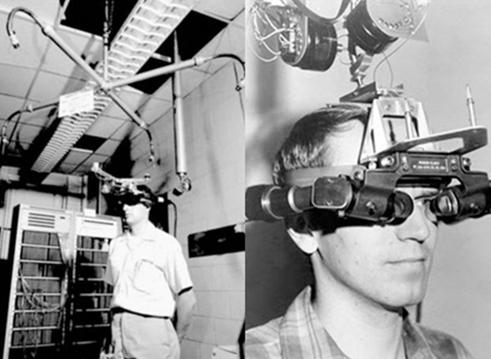
\includegraphics[width=0.5\textwidth]{figs/Sword-of-Damocles.png}
    \caption{Primer sistema RA: "Sword of Damocles" (1968)}
    \label{fig:sword_of_damocles}
\end{figure}

No obstante, el concepto formal de RA se desarrolló más tarde. En 1992, Caudell y Mizell acuñaron el término Augmented Reality en un contexto industrial, para referirse al uso de displays que asistían a operarios durante tareas complejas. Este enfoque pragmático orientó la investigación hacia sistemas útiles para tareas del mundo real, diferenciándose de la realidad virtual (RV), que propone la inmersión total en entornos digitales.

\subsection{Definición formal y primeros prototipos (1990–2000)}
Ronald Azuma estableció en 1997 la definición académica más citada de RA, basada en tres criterios fundamentales: (1) combinación de elementos reales y virtuales, (2) interacción en tiempo real y (3) registro espacial tridimensional preciso~\cite{azuma1997}. En paralelo, Paul Milgram y Fumio Kishino introdujeron el Continuo Realidad-Virtualidad, que posiciona la RA entre el entorno físico puro y la RV completa, permitiendo caracterizar distintos grados de mezcla entre ambos mundos~\cite{billinghurst2015}.

\begin{figure}[H]
    \centering
    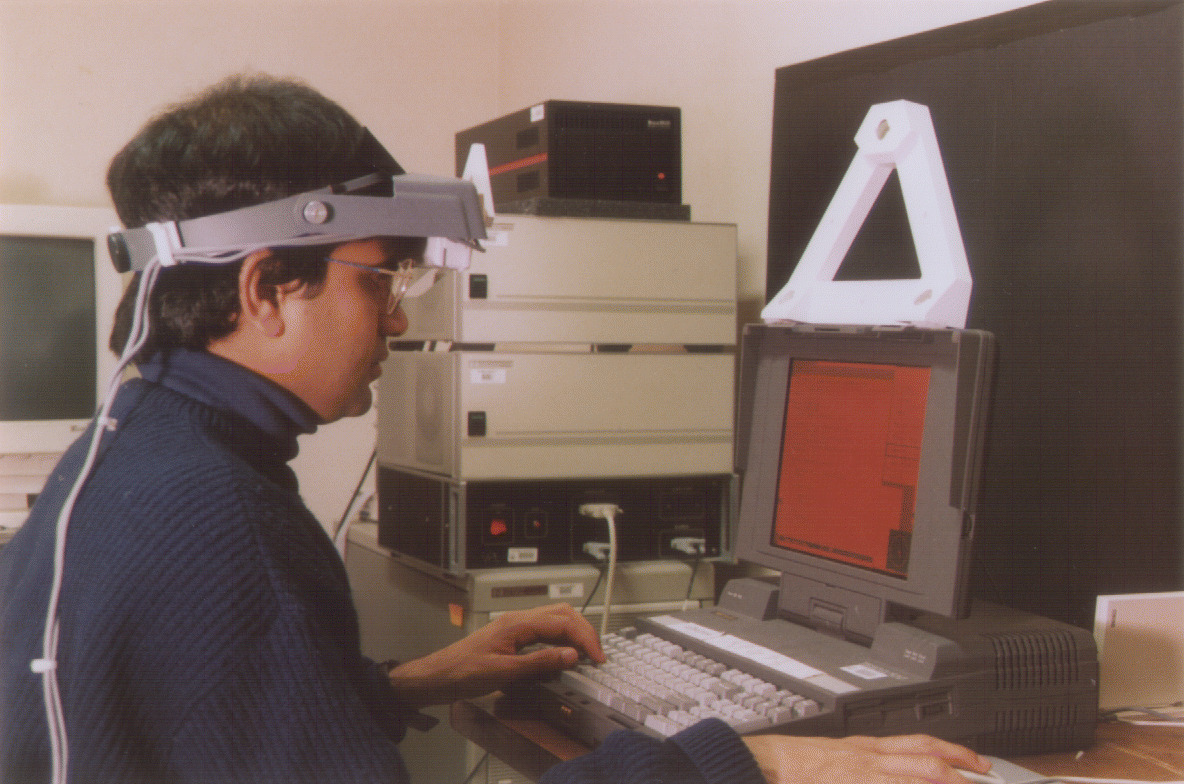
\includegraphics[width=0.6\textwidth]{figs/karma.jpg}
    \caption{Sistema KARMA para asistencia con RA (1993)}
    \label{fig:karma}
    % Fuente: Feiner et al., 1993
\end{figure}

Durante esta década se desarrollaron los primeros sistemas funcionales de RA. En 1993, el sistema KARMA, creado por Steve Feiner y su equipo, permitía la superposición de información contextual durante tareas físicas~\cite{feiner1993}. En 1997, se presentó el prototipo MARS, un sistema de RA móvil diseñado para guiar a turistas mediante visualización aumentada en tiempo real. Estas iniciativas fueron posibles gracias al desarrollo de dispositivos portables y técnicas de tracking visual.

\subsection*{Herramientas abiertas y salto a lo portátil (1999–2010)}
Uno de los hitos más relevantes en esta etapa fue el desarrollo de ARToolKit por Hirokazu Kato y Mark Billinghurst en 1999. Esta librería de código abierto permitió detectar marcadores visuales en video y superponer contenido digital 3D en tiempo real~\cite{kato1999}. Supuso una democratización de la RA, facilitando la experimentación por parte de investigadores y desarrolladores independientes.

\begin{figure}[H]
    \centering
    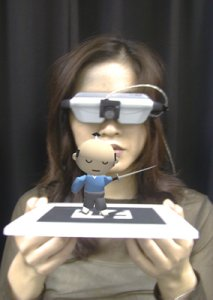
\includegraphics[width=0.3\textwidth]{figs/artoolkit.jpg}
    \caption{ARToolKit y marcadores visuales (1999)}
    \label{fig:artoolkit}
    % Fuente: Página del proyecto o artículo original
\end{figure}

Entre 2001 y 2004, surgieron los primeros sistemas de RA sobre dispositivos móviles, como PDAs y teléfonos inteligentes de primera generación. En 2003, Wagner y Schmalstieg presentaron un sistema de RA completamente autónomo en un dispositivo de mano~\cite{wagner2003}. Otros experimentos destacados fueron ARQuake (2000), un videojuego de RA en primera persona, y Invisible Train (2004), una aplicación colaborativa con varios usuarios simultáneos.


\section{La visibilización de las mujeres en el espacio urbano: una cuestión de justicia histórica}

La representación de las mujeres en el espacio urbano continúa siendo escasa. Según el proyecto europeo “Women’s Legacy”~\cite{womenslegacy2022}, impulsado desde la Conselleria d’Educació, Cultura i Esport de la Generalitat Valenciana, solo un 10\% de las calles con nombres de personas en muchas ciudades españolas están dedicadas a mujeres, y este patrón se repite en monumentos, placas conmemorativas y espacios simbólicos. 

A pesar de esta disparidad, en los últimos años han surgido iniciativas locales e institucionales orientadas a revertir esta situación. En Valencia, destaca el proyecto “Dones de Ciència”~\cite{lasnaves2020}, una colaboración entre la Universitat Politècnica de València (UPV) y Las Naves, que ha creado más de 30 murales urbanos en centros educativos para homenajear a mujeres científicas de todo el mundo. Esta intervención artística no solo embellece el entorno, sino que actúa como una herramienta pedagógica para inspirar a las nuevas generaciones. Asimismo, el Ayuntamiento de València ha promovido campañas de renombramiento de calles con nombres femeninos y la inclusión de mujeres en los itinerarios culturales y turísticos de la ciudad~\cite{ayuntamientovalencia2023}.

Por otra parte, diversas asociaciones vecinales y colectivos feministas han impulsado rutas autogestionadas por la ciudad que visibilizan las huellas femeninas en el espacio urbano. Entre ellas destaca la "Ruta Violeta de Mujeres en Valencia", organizada por la Asociación Por Ti Mujer, que recorre espacios emblemáticos ligados a la historia de las mujeres en la ciudad, promoviendo un reconocimiento público de sus contribuciones sociales y culturales~\cite{portimujer2023}.

Asimismo, la Assemblea Feminista de València ha organizado la "Ruta pels espais del Patronato de Protección a la Mujer", que recorre espacios vinculados a esta institución franquista, la cual operó durante gran parte del siglo XX bajo la tutela de la Iglesia y el Estado. Su función no era tanto proteger a mujeres víctimas de violencia como controlar y castigar a aquellas que transgredían los roles tradicionales de género. Esta ruta permite evidenciar cómo las estructuras institucionales legitimaron la exclusión, la represión y la estigmatización de mujeres consideradas "desviadas" por la moral conservadora, visibilizando así dinámicas de resistencia y memoria colectiva en la ciudad ~\cite{assemblea2023}.

Además, la "Ruta de Memorias Lesbianas", también organizada por la Assemblea Feminista de València, recorre lugares significativos para la comunidad lésbica, con el objetivo de visibilizar los derechos y experiencias de las mujeres lesbianas en la Valencia de los años 70, 80 y 90, destacando la importancia de reconocer y valorar estas luchas en la construcción de la historia urbana~\cite{assemblea2024}.

Estas rutas permiten redescubrir barrios desde una óptica feminista, incorporando historias personales, luchas sociales y legados invisibilizados. En este sentido, la plataforma DONA’m MÓN podría ser un recurso útil a implementar durante estas rutas, integrando información geolocalizada, recursos multimedia y facilitando la participación activa de las personas en la construcción de esta memoria feminista urbana. 


\subsection{Referentes femeninos en la ciudad: biografías y puntos de interés}

La aplicación propuesta busca poner en valor la figura de mujeres que, desde distintos campos del saber y la acción, han contribuido de manera decisiva al progreso de los derechos, el pensamiento y la cultura. Aunque muchas de ellas han nacido o trabajado en Valencia, su legado trasciende el ámbito local y constituye una aportación fundamental a la historia del feminismo y la igualdad. A través de la geolocalización de lugares clave asociados a sus vidas y obras, se propone una experiencia que va más allá de la información enciclopédica, para convertirse en un ejercicio de reconocimiento social y emocional de su presencia en la ciudad.

Una de las figuras destacadas es Concepción Aleixandre Ballester (1862–1952), una de las primeras mujeres médicas en España y pionera en el ámbito de la ginecología. Su activismo feminista se centró en la defensa del acceso de las mujeres a la educación y al ejercicio profesional de la medicina, algo profundamente innovador en su tiempo. Estudió en la Universidad de Valencia, donde enfrentó obstáculos institucionales por su condición de mujer, y desarrolló una intensa carrera médica y científica. El edificio histórico de la Facultad de Medicina de la Universitat de València es un lugar simbólico para recordar su figura y su lucha por la igualdad en el ámbito sanitario~\cite{guijarro2021}.

Otra mujer fundamental en la historia reciente de Valencia es Carmen Alborch (1947–2018). Fue ministra de Cultura, escritora, catedrática de Derecho Mercantil y una de las voces más influyentes del feminismo institucional en España. Su obra literaria, como \textit{Solas} (1999), promovió un feminismo humanista accesible y empático. En Valencia, dejó una impronta profunda como directora del Instituto Valenciano de Arte Moderno (IVAM), donde impulsó una política cultural abierta, plural y comprometida con la igualdad. El IVAM, por tanto, no solo representa su labor como gestora cultural, sino también su apuesta por un feminismo integrador desde las instituciones~\cite{alborch1999}.

En el ámbito de los derechos civiles, Clara Campoamor (1888–1972) ocupa un lugar esencial por su incansable lucha por el sufragio femenino, que logró defender con éxito en las Cortes Constituyentes de 1931. Si bien no tuvo una vinculación directa con Valencia, su legado ideológico inspiró a generaciones de mujeres en toda España, incluida la Comunidad Valenciana. La existencia de centros educativos como el CEIP Clara Campoamor subraya la importancia de su figura como referente pedagógico y su impacto en la formación de una conciencia feminista desde edades tempranas~\cite{gonzalez2006}.

Retrocediendo a la Edad Media, encontramos a Isabel de Villena (1430–1490), abadesa del Real Monasterio de la Trinidad y considerada la primera escritora en lengua valenciana. Su obra \textit{Vita Christi} constituye una relectura humanista del relato evangélico desde una perspectiva femenina, resaltando la figura de la Virgen y otras mujeres bíblicas. Isabel de Villena transformó el espacio monástico en un lugar de producción intelectual y espiritual liderado por mujeres, algo excepcional en su época. El Monasterio de la Trinidad, donde vivió y escribió, es un lugar clave para reivindicar la aportación femenina a la literatura y la espiritualidad valencianas~\cite{rueda2013}.

En la medicina, Manuela Solís Clarás (1888–1936) destaca por ser una de las primeras mujeres médicas de la ciudad. Ejerció en el Hospital Provincial de Valencia y fue una firme defensora del acceso de las mujeres a la formación sanitaria. Además de su práctica médica, se implicó en la divulgación científica y en la promoción de redes de apoyo entre profesionales sanitarias, en un momento en que la medicina era un espacio profundamente masculinizado~\cite{martinez2019}. El Hospital Provincial es, por tanto, un espacio idóneo para recordar su legado.

La aplicación también incluye representaciones artísticas contemporáneas de mujeres de gran relevancia internacional. Por ejemplo, Mae Jemison, primera mujer afroamericana en viajar al espacio, es homenajeada con un mural en el CEIP Torrefiel. Su figura simboliza la superación de barreras raciales y de género en los campos de la ciencia y la exploración espacial. Del mismo modo, Vandana Shiva, ecofeminista india y activista medioambiental, cuenta con un mural en el CEIP Ballester Fandos. Su lucha por la justicia ambiental, la soberanía alimentaria y los derechos de las mujeres rurales conecta con un feminismo global que también debe tener presencia en las narrativas educativas locales~\cite{shiva2005}.

“DONA’m MÓN” busca ser un vehículo para visibilizar la presencia de estas figuras en el espacio urbano, contribuyendo así a una representación más justa y equitativa de la historia y promoviendo un futuro en el que la diversidad y la igualdad sean valores fundamentales.

\begin{figure}[H]
    \centering
    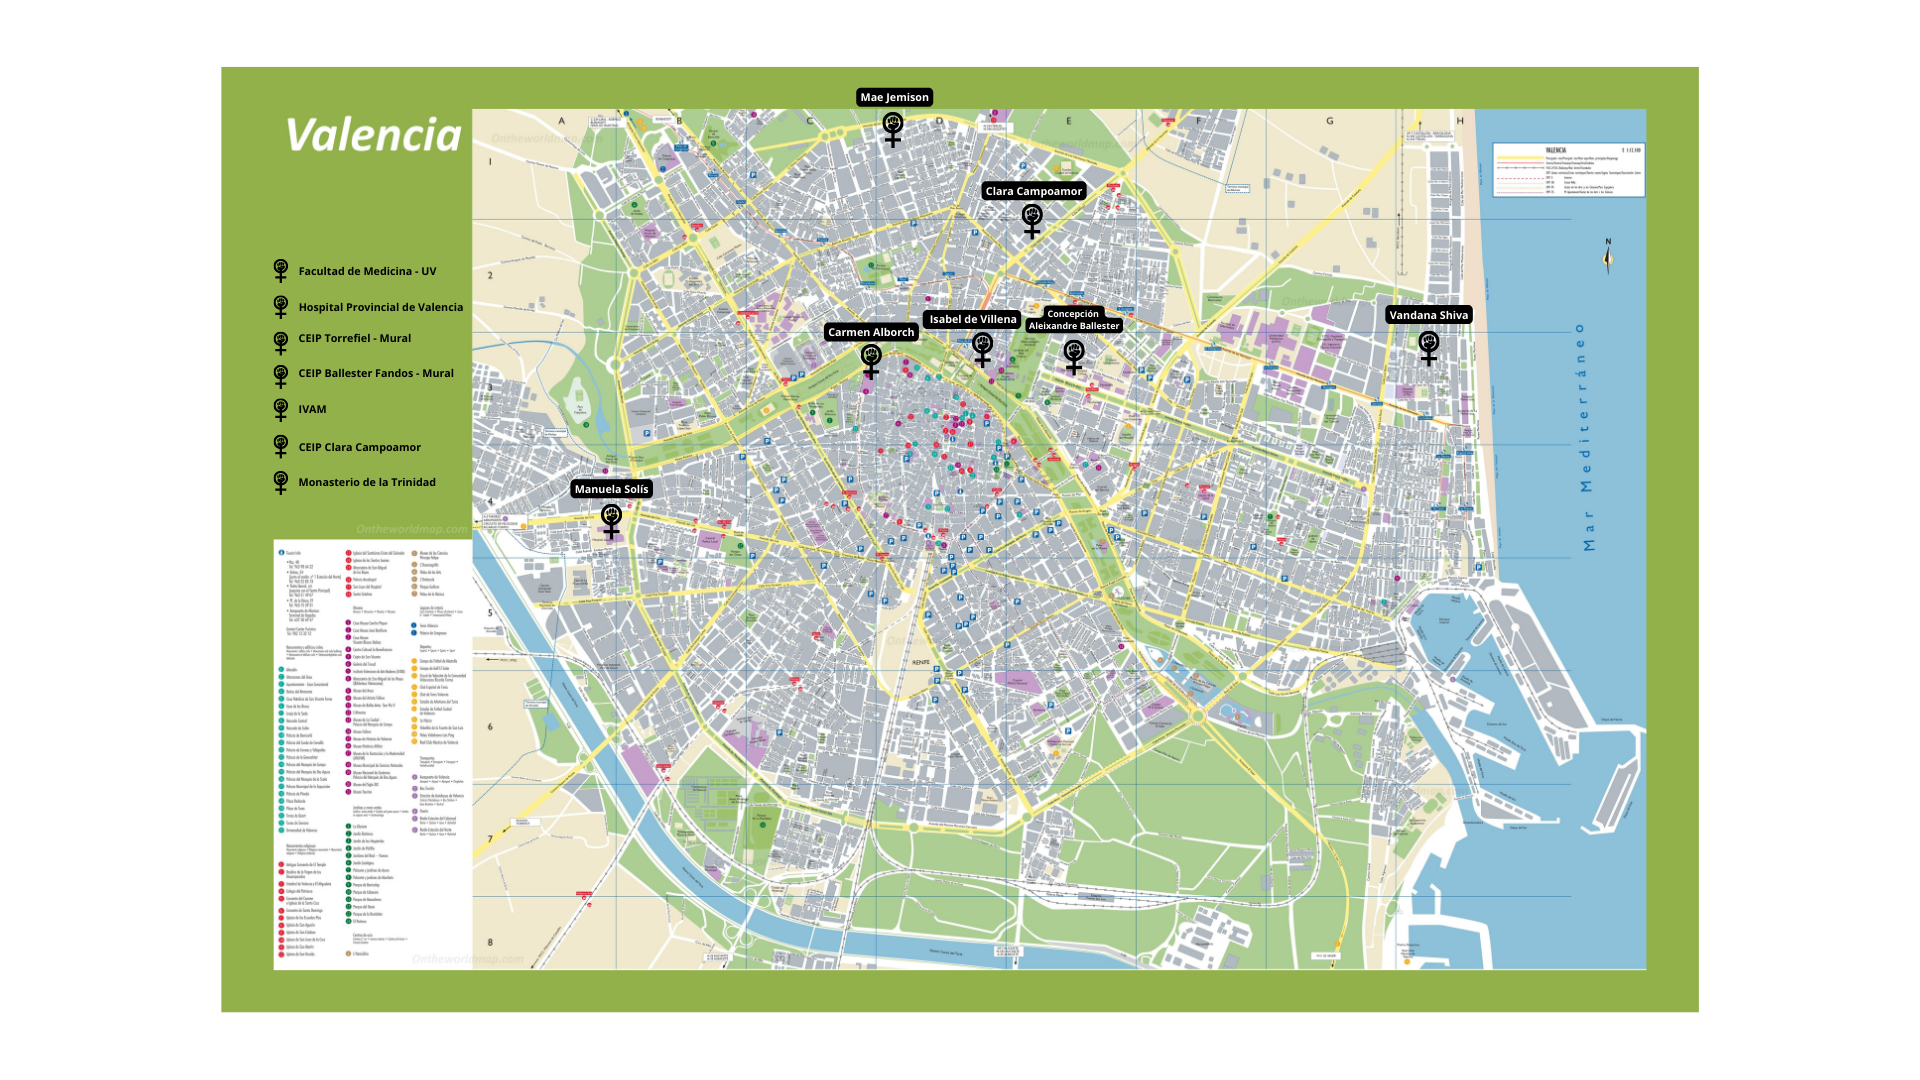
\includegraphics[width=\textwidth]{figs/mapa.png}
    \caption{Mapa de Valencia con los puntos geolocalizados de las mujeres referentes incluidos en la aplicación.}
    \label{fig:mapa_valencia_mujeres}
\end{figure}



\section{Análisis de aplicaciones similares}
% Qué aplicaciones similares hay y en qué se diferencia de ellas la propuesta

En el desarrollo de “DONA’m MÓN”, resulta esencial analizar aplicaciones existentes que, de manera similar, combinan geolocalización y realidad aumentada (RA) para ofrecer experiencias inmersivas y educativas. Este análisis nos permite identificar características, estrategias y tecnologías clave que podrían ser adaptadas para cumplir con los objetivos específicos del proyecto. A continuación, se presentan algunas aplicaciones relevantes cuyos enfoques, funcionalidades y tecnologías han inspirado aspectos concretos del diseño conceptual de este TFG.

\subsubsection{Pokémon GO}

Una de las referencias más notables es Pokémon GO, que revolucionó el mercado de aplicaciones móviles al combinar geolocalización y RA para motivar a los usuarios a explorar el mundo real. En este caso, los jugadores buscan y capturan criaturas virtuales que aparecen en puntos geográficos específicos. La aplicación también implementa un sistema de recompensas y niveles que fomenta la participación constante. Aunque el enfoque principal de Pokémon GO es el entretenimiento, su éxito demuestra cómo las tecnologías inmersivas pueden transformar la forma en que las personas interactúan con su entorno. En “DONA’m MÓN”, se busca adaptar esta dinámica de exploración y descubrimiento, pero con un enfoque educativo y cultural, utilizando los puntos de interés como portales hacia las historias de mujeres que dejaron una huella significativa en Valencia.

\begin{figure}[H]
    \centering
    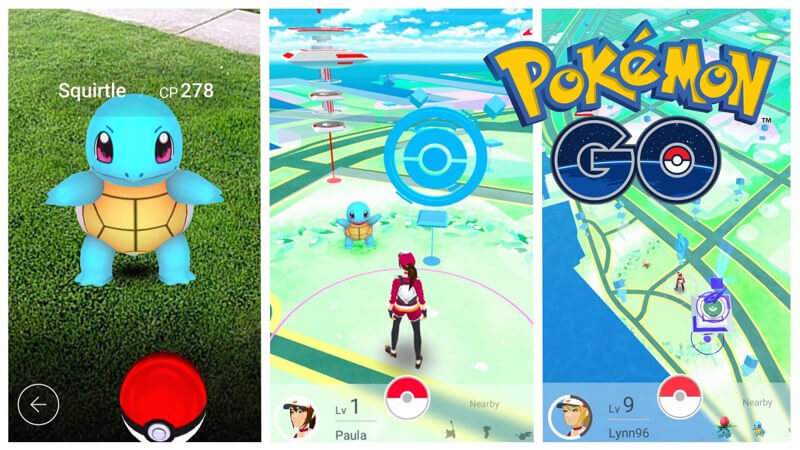
\includegraphics[width=0.5\textwidth]{figs/pokemon_go.jpg}
    \caption{Interfaz de Pokémon GO mostrando un entorno real aumentado con la aparición de un Pokémon virtual y también el entorno virtual del juego.}
    \label{fig:pokemon_go}
\end{figure}

\subsubsection{Streetmuseum}

Por otro lado, Streetmuseum es una aplicación que también aprovecha la RA, pero con un objetivo más centrado en la historia y la cultura. Esta herramienta permite a los usuarios visualizar imágenes y escenas históricas superpuestas al paisaje actual, ofreciendo una perspectiva del pasado en tiempo real. La capacidad de conectar visualmente el entorno moderno con eventos y figuras históricas es una inspiración directa para el proyecto. En nuestro proyecto, esta idea se adapta al permitir que los usuarios accedan a contenido multimedia –como imágenes, textos y modelos 3D– que contextualice la vida y obra de las mujeres en cada ubicación geolocalizada.

\begin{figure}[H]
    \centering
    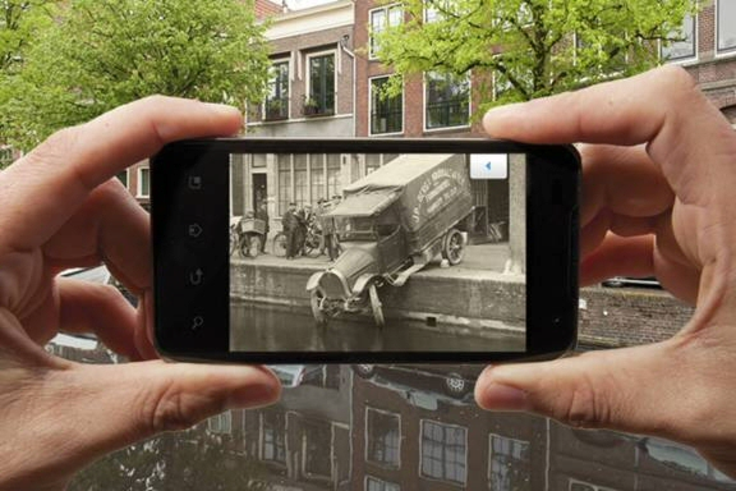
\includegraphics[width=0.5\textwidth]{figs/streetmuseum.png}
    \caption{Ejemplo de Streetmuseum: visualización de una escena histórica superpuesta sobre el entorno actual de la ciudad.}
    \label{fig:streetmuseum}
\end{figure}

\subsubsection{CultuAR}

CultuAR, desarrollada por la empresa española AR Vision, es una aplicación que combina la geolocalización con la realidad aumentada para ofrecer visitas culturales interactivas en más de 200 municipios. Mediante la cámara del dispositivo, los usuarios pueden visualizar reconstrucciones históricas, personajes del pasado o información multimedia superpuesta al entorno real. Una de sus características más valiosas es la capacidad de personalizar rutas culturales por municipios, integrando elementos inmersivos que enriquecen la experiencia turística y patrimonial. Esta aplicación destaca por su integración fluida con el entorno urbano y su enfoque didáctico, lo que representa una clara inspiración para DONA'm MÓN en cuanto a accesibilidad y diseño de experiencias geolocalizadas con RA.

\begin{figure}[H]
    \centering
    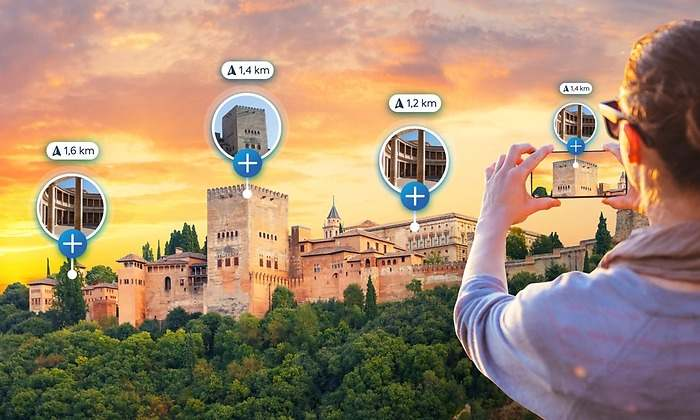
\includegraphics[width=0.5\textwidth]{figs/cultuar.jpeg}
    \caption{Captura de CultuAR mostrando información sobre un monumento en el entorno real.}
    \label{fig:cultuar}
\end{figure}

\subsubsection{Historypin}

Finalmente, Historypin se presenta como una plataforma colaborativa que permite a los usuarios subir y explorar fotografías, eventos y recuerdos históricos asociados a ubicaciones específicas. Lo más destacable de esta aplicación es su enfoque participativo, donde los usuarios pueden contribuir activamente al contenido disponible. Este modelo de colaboración inspira la posibilidad de que, en futuras versiones de “DONA’m MÓN”, los usuarios también puedan agregar información o enriquecer las narrativas existentes sobre mujeres de Valencia, convirtiendo la aplicación en una herramienta dinámica y viva.

\begin{figure}[H]
    \centering
    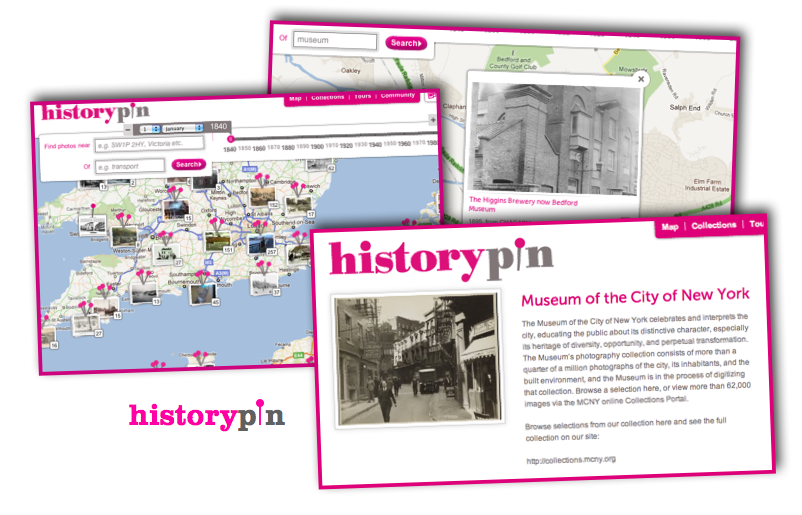
\includegraphics[width=0.5\textwidth]{figs/history-pin.png}
    \caption{Interfaz de Historypin donde se visualizan fotografías históricas asociadas a ubicaciones reales en el mapa y su detalle de contenido.}
    \label{fig:historypin}
\end{figure}
\subsubsection{}

Estas cuatro aplicaciones ilustran diversas maneras de utilizar la tecnología para crear experiencias inmersivas e interactivas. Cada una de ellas presenta fortalezas únicas que se alinean, en mayor o menor medida, con los objetivos de DONA'm MÓN. De Pokémon GO tomamos la dinámica de exploración y gamificación; de Streetmuseum, la idea de superponer contenido histórico en el entorno actual; de CultuAR, el uso efectivo de RA para la divulgación cultural local; y de Historypin, el potencial de colaboración comunitaria. Esta combinación de estrategias y conceptos pretende hacer de DONA'm MÓN una aplicación única que conecte a los usuarios con la historia de manera inclusiva, educativa e innovadora.



\section{Tecnologías}
% Análisis crítico de las tecnologías y sistemas de despliegue posibles y por qué se han seleccionado unas concretas.
En este apartado se analizan las tecnologías disponibles y las soluciones existentes en el mercado que pueden ser aplicadas al desarrollo de la aplicación móvil. Este análisis incluye una revisión de herramientas de geolocalización, realidad aumentada, bases de datos y frameworks de desarrollo multiplataforma. La selección de las tecnologías se justifica considerando la funcionalidad, compatibilidad y eficiencia necesarias para cumplir con los objetivos del proyecto.

\subsection{Plataformas de desarrollo de aplicaciones móviles}

Una de las decisiones fundamentales en cualquier proyecto de ingeniería de software es la elección de la tecnología base sobre la cual se construirá la aplicación. Esta decisión afecta directamente a la arquitectura general, la experiencia de usuario, la mantenibilidad del código y la escalabilidad futura del sistema. En el contexto de este proyecto, se evaluaron varias opciones para el desarrollo de una aplicación móvil multiplataforma que integrase geolocalización, funcionalidades de realidad aumentada, y una interfaz moderna, accesible y responsiva.

\textbf{Unity.} Unity es un motor de desarrollo multiplataforma ampliamente utilizado en los ámbitos del videojuego, simulación y experiencias interactivas en tiempo real. Su potencia radica en su motor gráfico, que permite renderizar contenido 3D de alta calidad, así como en su flexibilidad para implementar lógica de aplicación mediante scripts en C\#. Unity ofrece soporte directo para tecnologías de realidad aumentada a través de módulos como AR Foundation, que actúan como capa de abstracción sobre ARKit (iOS) y ARCore (Android), permitiendo así desarrollar una única base de código RA para múltiples plataformas.

En lo relativo a interfaces de usuario, Unity ha evolucionado en los últimos años. Su sistema tradicional basado en el Canvas permitía crear interfaces gráficas bidimensionales, pero con limitaciones de estilo y escalabilidad. Como respuesta a estas deficiencias, se introdujo UI Toolkit, un nuevo sistema de interfaz basado en un modelo declarativo, inspirado en tecnologías web como HTML y CSS. UI Toolkit permite separar la lógica de presentación del comportamiento, definiendo componentes visuales reutilizables y estilos en archivos dedicados. A pesar de estas mejoras, el desarrollo de interfaces ricas, formularios interactivos y navegación compleja continúa siendo menos eficiente que en frameworks específicos para aplicaciones móviles.

\textbf{React Native.} React Native es un framework desarrollado por Meta (anteriormente Facebook) para el desarrollo de aplicaciones móviles multiplataforma utilizando JavaScript y el modelo de componentes de React. Permite crear interfaces de usuario nativas reutilizando componentes declarativos que se renderizan mediante puentes hacia los componentes nativos de Android e iOS. Una de las grandes ventajas de React Native es su arquitectura reactiva, que permite gestionar estados complejos de forma eficiente, manteniendo la UI sincronizada con los datos de la aplicación.

En combinación con Expo, un conjunto de herramientas que facilita la creación y prueba de aplicaciones React Native, es posible desarrollar aplicaciones sin necesidad de compilar ni configurar código nativo. Esto permite utilizar herramientas como Expo Go para probar la aplicación directamente en un dispositivo físico mediante código QR, lo que acelera significativamente el flujo de desarrollo. React Native es especialmente potente para construir interfaces modernas, personalizadas y adaptables, con soporte para navegación compleja, formularios, animaciones y estilos dinámicos.

\textbf{Flutter.} Flutter es un framework desarrollado por Google para construir aplicaciones multiplataforma desde una única base de código. Utiliza el lenguaje Dart, y su arquitectura se basa en un sistema de renderizado propio que dibuja todos los elementos de la UI desde cero, lo que garantiza uniformidad visual entre plataformas. Flutter ofrece una amplia colección de widgets personalizables y anima la creación de interfaces complejas de forma declarativa y eficiente.

Aunque Flutter no fue la opción elegida para este proyecto, se considera una alternativa competitiva frente a React Native. Sin embargo, su adopción requiere dominar el lenguaje Dart, y su integración con tecnologías de realidad aumentada aún está en evolución en comparación con la madurez del ecosistema de Unity o la compatibilidad simplificada que ofrece React Native con herramientas web como AR.js y A-Frame.

\textbf{Desarrollo de interfaz de usuario y elección final.} Una parte crucial del proyecto es la interfaz gráfica de usuario, dado que la aplicación está destinada a un público general y debe facilitar la navegación intuitiva, la visualización de datos geográficos y el acceso a contenidos de realidad aumentada. Si bien Unity, especialmente con UI Toolkit, ofrece un entorno funcional para construir interfaces gráficas, su enfoque está más orientado a interacciones en entornos tridimensionales y menos a la gestión de flujos de navegación o formularios comunes en aplicaciones móviles.

Por el contrario, React Native destaca precisamente en este tipo de interfaz. Su modelo declarativo, su sistema de componentes reutilizables, su integración con herramientas modernas de desarrollo (como React Navigation, Redux o Context API), y su compatibilidad con Expo, permiten construir aplicaciones móviles escalables y con una experiencia de usuario optimizada.

Por estos motivos, y tras un análisis técnico detallado, se decidió utilizar React Native con Expo como entorno principal de desarrollo para esta aplicación, reservando el uso de tecnologías gráficas (como la realidad aumentada) a componentes embebidos que se integran dentro de esta arquitectura general. Esta elección permite combinar la robustez de React para la UI con la flexibilidad de integrar experiencias multimedia mediante tecnologías web.

\subsection{Geolocalización}

La geolocalización es uno de los pilares fundamentales de la aplicación, ya que permite situar puntos de interés específicos en un mapa, facilitando que los usuarios exploren la ciudad de Valencia mientras descubren la historia de mujeres destacadas. Para implementar esta funcionalidad, existen diversas herramientas ampliamente utilizadas en el desarrollo de aplicaciones móviles:

\begin{itemize}
    \item \textbf{Google Maps API}: Es una solución robusta y versátil que permite integrar mapas interactivos, obtener datos de ubicación en tiempo real y personalizar la visualización según las necesidades del proyecto. Ofrece documentación detallada y soporte técnico, lo que facilita su integración. Sin embargo, su principal desventaja es que su plan gratuito únicamente se ofrece durante un periodo de prueba de corta duración y su coste se incrementa en proyectos con un gran volumen de usuarios o solicitudes~\cite{googlemaps2024}.
    \item \textbf{Mapbox}: Alternativa potente que combina funcionalidades avanzadas, un alto nivel de personalización estética y una política de precios más flexible que Google Maps API, ya que su plan gratuito no tiene un límite de tiempo. Es especialmente útil en aplicaciones que requieren un diseño visual distintivo. No obstante, su integración puede resultar más compleja para desarrolladores con poca experiencia~\cite{mapbox2024}.
    \item \textbf{OpenStreetMap (OSM)}: Opción de código abierto que permite el acceso y uso gratuito de datos cartográficos, además de ofrecer un alto nivel de personalización. Esta plataforma colaborativa es especialmente adecuada para proyectos con presupuestos limitados o académicos, ya que no implica costes de licencia. Aunque carece de algunas funcionalidades avanzadas nativas, como el enrutamiento en tiempo real o servicios de geolocalización enriquecidos, su flexibilidad y libertad de uso la convierten en una solución funcional y accesible~\cite{osm2024}.
    \item \textbf{Mapas nativos del dispositivo con React Native}: Esta opción permite aprovechar las capacidades de geolocalización del propio sistema operativo del dispositivo móvil (iOS o Android) mediante bibliotecas como react-native-maps. Es una solución eficiente y ligera, que facilita la integración con el hardware del dispositivo y proporciona una experiencia fluida. Además, evita costes derivados de servicios externos, lo que la convierte en una alternativa atractiva para proyectos con recursos limitados~\cite{reactnativemaps2024}.
\end{itemize}

En este proyecto se ha optado por utilizar mapas nativos con React Native, ya que permiten una integración directa con la aplicación móvil, ofrecen un rendimiento óptimo, y eliminan la dependencia de servicios externos de pago. Esta elección responde a criterios de eficiencia, sostenibilidad económica y control sobre el desarrollo.

\subsection{Realidad Aumentada (RA)}

Una vez definida la arquitectura general de la aplicación y confirmado el uso de React Native como entorno principal de desarrollo, fue necesario analizar detalladamente qué tecnologías de realidad aumentada (RA) podían integrarse de forma eficiente, respetando las limitaciones del ecosistema de desarrollo adoptado. Uno de los objetivos fundamentales era conservar la compatibilidad con Expo Go, evitando procesos de compilación nativa que dificultasen el flujo de desarrollo iterativo. Bajo esta premisa, se realizó un estudio de las distintas alternativas existentes, evaluando tanto su madurez técnica como su grado de integración con React Native.

\textbf{Realidad aumentada con tecnologías nativas.}
Las soluciones nativas ofrecen, en general, el mayor grado de precisión, rendimiento y acceso a capacidades avanzadas del dispositivo. Entre estas destacan ARKit (para dispositivos iOS) y ARCore (para Android), los kits de desarrollo oficial proporcionados por Apple y Google, respectivamente. Ambas plataformas permiten el seguimiento del entorno, la detección de planos horizontales y verticales, la oclusión de objetos virtuales con respecto al entorno físico, el anclaje espacial y la iluminación adaptativa. Estas herramientas están diseñadas para crear experiencias inmersivas de alta calidad y son ampliamente utilizadas en entornos profesionales y comerciales.

Sin embargo, una de sus limitaciones fundamentales es su naturaleza monoplataforma. Para desarrollar una aplicación de RA que funcione tanto en Android como en iOS, sería necesario implementar dos versiones independientes, o bien utilizar un entorno unificador como Unity, que permite compilar una única base de código para múltiples sistemas operativos.

Unity, a través de su módulo AR Foundation, permite abstraer las diferencias entre ARKit y ARCore, y desarrollar experiencias RA multiplataforma con una arquitectura común. Unity es particularmente potente en términos de renderizado gráfico, gestión de modelos tridimensionales, simulación física y animación en tiempo real, por lo que constituye una de las herramientas más robustas para el desarrollo de RA avanzada.

No obstante, su integración con aplicaciones desarrolladas en React Native es compleja. El enfoque convencional implicaría desarrollar toda la aplicación en Unity, lo cual, como se ha discutido anteriormente, penaliza la usabilidad y escalabilidad de la interfaz. Por este motivo, se exploró también la posibilidad de utilizar Unity como una librería nativa embebida dentro de una aplicación React Native.

\textbf{Unity como librería nativa integrada en React Native.}
Unity permite exportar un proyecto como una librería nativa —un archivo .aar para Android o .framework para iOS— que puede integrarse dentro de una aplicación móvil desarrollada con otras tecnologías, como React Native. Este enfoque, conocido como Unity as a Library, ofrece la posibilidad de desarrollar únicamente la parte de RA en Unity y exponerla como un módulo invocable desde la aplicación principal.

Mediante este patrón arquitectónico, es posible mantener la lógica general y la interfaz de usuario desarrolladas en React Native, y delegar en Unity únicamente el renderizado y gestión de la escena RA. La comunicación entre ambos entornos se realiza mediante puentes nativos que deben implementarse en Java/Kotlin (para Android) y Objective-C/Swift (para iOS).

Este enfoque ha sido demostrado en proyectos como react-native-unity, que ofrecen ejemplos funcionales de integración, así como en la documentación oficial de Unity (Unity as a Library). No obstante, esta integración presenta múltiples desafíos técnicos:

\begin{itemize}
    \item Es necesario ejectar el proyecto Expo, abandonando así la posibilidad de utilizar Expo Go y el flujo de desarrollo simplificado que ofrece.
    \item La configuración del proyecto requiere conocimientos avanzados en desarrollo nativo para cada plataforma.
    \item La integración y sincronización de eventos entre Unity y React Native debe implementarse manualmente.
\end{itemize}

Por tanto, aunque Unity como librería nativa representa una solución muy potente desde el punto de vista gráfico y funcional, su coste de integración y mantenimiento dentro de una arquitectura basada en React Native la convierte en una opción poco viable para este proyecto, cuyo foco está en la accesibilidad, rapidez de desarrollo y compatibilidad multiplataforma sin compilación nativa.

\textbf{Realidad aumentada en React Native con tecnologías web.}
En busca de una alternativa más ligera y plenamente compatible con React Native y Expo, se optó por explorar las soluciones basadas en tecnologías web. Una de las más destacadas es AR.js, una librería de código abierto que permite implementar experiencias de RA directamente en navegadores móviles, sin necesidad de acceso a capas nativas. AR.js se basa en WebGL, Three.js y A-Frame, y permite implementar RA sobre marcadores visuales (marker-based AR) mediante la detección de patrones gráficos como Hiro, Kanji o diseños personalizados.

Complementando AR.js, el framework A-Frame facilita la construcción declarativa de escenas 3D y RA mediante HTML. Permite importar modelos .glb, añadir iluminación, cámaras, interacciones y animaciones sin necesidad de escribir código complejo de bajo nivel. Esta aproximación reduce significativamente la barrera de entrada al desarrollo de RA, y se adapta perfectamente al modelo de desarrollo web moderno.

Las escenas construidas con A-Frame y AR.js pueden ser desplegadas como aplicaciones web estáticas (por ejemplo, en GitHub Pages), e integradas dentro de la aplicación React Native utilizando el componente WebView, que actúa como un navegador embebido. Este enfoque permite mantener la lógica general y la interfaz de la aplicación dentro del ecosistema de React Native, mientras que la experiencia de RA se encapsula como una unidad independiente, reutilizable y fácilmente actualizable.

\textbf{Viro React.}
Otra alternativa evaluada fue Viro React, un framework orientado a la creación de experiencias inmersivas en RA y realidad virtual directamente en React Native. Viro permite cargar modelos 3D, definir cámaras, aplicar animaciones, detectar superficies, y renderizar objetos virtuales en función del entorno físico. Su enfoque declarativo está alineado con la filosofía de React y ofrece un entorno de desarrollo intuitivo para experiencias visuales.

No obstante, Viro no es compatible con Expo Go, ya que depende de módulos nativos que requieren compilar la aplicación. Para utilizarlo, es necesario ejectar el proyecto y utilizar herramientas como EAS Build para generar versiones personalizadas de la app. Esta necesidad de compilación rompe el flujo de desarrollo ágil basado en Expo y contradice uno de los principios técnicos fundamentales del proyecto: evitar configuraciones nativas complejas para preservar la portabilidad y escalabilidad del sistema.

\textbf{Elección final.}
Después de un análisis riguroso, se optó por utilizar AR.js combinado con A-Frame, integrados en la aplicación React Native mediante un componente WebView. Esta solución permite cumplir los objetivos funcionales de la aplicación (visualización de modelos 3D sobre marcadores físicos), respetando al mismo tiempo los requisitos técnicos del entorno (compatibilidad con Expo, desarrollo ágil, y arquitectura limpia).

La elección de esta tecnología responde a criterios técnicos sólidos:

\begin{itemize}
    \item Portabilidad total: la experiencia RA se ejecuta en el navegador y es accesible desde cualquier dispositivo moderno.
    \item Desacoplamiento arquitectónico: la escena RA es independiente del código base de la aplicación.
    \item Facilidad de mantenimiento: se pueden actualizar las escenas de RA sin necesidad de recompilar la app.
    \item Compatibilidad con Expo Go: se preserva el flujo de desarrollo iterativo y multiplataforma.
\end{itemize}

En resumen, esta arquitectura permite combinar las ventajas del desarrollo móvil moderno (mediante React Native) con la flexibilidad de tecnologías web para RA, consiguiendo una solución técnica equilibrada, funcionalmente completa y sostenible a largo plazo.

\subsection{Base de Datos}

\subsection{Arquitectura de persistencia y gestión de datos}

En el desarrollo de esta aplicación se ha optado por una arquitectura desacoplada que separa claramente el frontend y el backend. El frontend se implementa en React Native, lo que permite el despliegue multiplataforma en dispositivos móviles, mientras que el backend se desarrolla en Django, un framework web de alto nivel que facilita la creación de aplicaciones robustas y seguras~\cite{django2024}.

\subsubsection{Persistencia de datos en entornos relacionales y no relacionales}

La persistencia de datos es un aspecto fundamental en el desarrollo de aplicaciones que requieren almacenar información de manera duradera. Existen dos enfoques principales para gestionar esta persistencia: las bases de datos relacionales, que estructuran la información en tablas con relaciones definidas mediante claves, y las bases de datos no relacionales, que permiten una mayor flexibilidad al almacenar los datos en formatos como documentos, grafos o pares clave-valor~\cite{elmasri2017}. 

Las bases de datos relacionales son especialmente adecuadas cuando los datos presentan una estructura definida, relaciones entre entidades y necesidad de integridad referencial, mientras que las no relacionales ofrecen ventajas en contextos donde la escalabilidad horizontal, la alta disponibilidad o la variabilidad en los esquemas de datos son prioritarias~\cite{stonebraker2011}.

\subsubsection{Django y la arquitectura MVT}

Django se basa en la arquitectura Modelo–Vista–Plantilla (MVT), un patrón similar al clásico MVC (Model–View–Controller), adaptado al ecosistema web de Python~\cite{vincent2020}. Este patrón organiza el código en tres componentes:

\begin{itemize}
    \item \textbf{Modelo (Model):} Define la estructura de los datos y su comportamiento a través de clases Python, que se traducen automáticamente en tablas mediante el ORM (Object-Relational Mapping) de Django.
    \item \textbf{Vista (View):} Gestiona la lógica de negocio y responde a las solicitudes HTTP, procesando la información que llega desde el frontend.
    \item \textbf{Plantilla (Template):} Presenta la información al usuario utilizando HTML enriquecido con etiquetas dinámicas, aunque en este proyecto su papel es mínimo, ya que la interfaz se renderiza completamente en React Native.
\end{itemize}

La interacción entre Django y la base de datos está mediada por su ORM, lo que permite manipular los datos mediante objetos Python en lugar de consultas SQL explícitas. Esta capa de abstracción incrementa la seguridad —previniendo ataques como la inyección SQL— y facilita el mantenimiento del código~\cite{vincent2020}.

\subsubsection{Sistema de Gestión de Bases de Datos: MySQL}

Para este proyecto se ha elegido MySQL como sistema de gestión de bases de datos relacional (SGBDR), debido a su madurez, rendimiento y plena compatibilidad con Django~\cite{oracle2023}. MySQL permite estructurar los datos de manera eficiente y soporta operaciones complejas con múltiples relaciones entre tablas, lo que resulta fundamental para gestionar tanto la información relacionada con las figuras históricas como los datos de geolocalización, multimedia y analíticas del uso de la app.

La configuración entre Django y MySQL se realiza mediante el uso de controladores compatibles (como \texttt{mysqlclient}), lo que asegura una integración fluida y un rendimiento óptimo.

\subsubsection{Comparativa entre sistemas de bases de datos}

A continuación se muestra una tabla comparativa entre los principales sistemas de gestión de bases de datos considerados:

\begin{table}[H]
    \centering
    \begin{tabular}{|l|c|c|c|c|}
        \hline
        \textbf{Característica} & \textbf{SQLite} & \textbf{MySQL} & \textbf{MariaDB} & \textbf{MongoDB} \\ \hline
        Tipo & Relacional & Relacional & Relacional & No relacional \\ \hline
        Escalabilidad & Baja & Alta & Alta & Muy alta \\ \hline
        Rendimiento & Medio & Alto & Muy alto & Alto \\ \hline
        Integridad referencial & Sí & Sí & Sí & No \\ \hline
        Compatibilidad Django & Nativa & Completa & Completa & Parcial (con plugins) \\ \hline
        Flexibilidad de esquema & Baja & Media & Media & Alta \\ \hline
        Facilidad de configuración & Muy fácil & Media & Media & Media \\ \hline
        Comunidad y soporte & Moderada & Muy activa & Activa & Muy activa \\ \hline
    \end{tabular}
    \caption{Comparativa entre SQLite, MySQL, MariaDB y MongoDB~\cite{elmasri2017, mariadb2023, mongodb2024}.}
    \label{tabla:comparativa_bases_datos}
\end{table}

\subsubsection{Consideraciones sobre otras tecnologías: MariaDB, SQLite, MongoDB y Cassandra}

Aunque inicialmente se contempló el uso de MariaDB, una bifurcación de MySQL con mejoras en rendimiento y licencias completamente abiertas, finalmente se optó por MySQL por razones de compatibilidad institucional y soporte técnico~\cite{mariadb2023}. SQLite, si bien está soportada nativamente por Django y resulta útil en fases de desarrollo o en aplicaciones de bajo requerimiento, no ofrece la escalabilidad ni la gestión de concurrencia necesarias para este proyecto~\cite{django_sqlite2024}. 

En cuanto a las bases de datos no relacionales, cabe mencionar tecnologías como MongoDB y Cassandra. MongoDB, basada en documentos JSON, es ampliamente utilizada en aplicaciones que requieren estructuras de datos flexibles y cambios frecuentes en el esquema~\cite{mongodb2024}. Cassandra, por su parte, está orientada a entornos distribuidos con grandes volúmenes de datos y alta disponibilidad~\cite{cassandra2023}. Sin embargo, el enfoque relacional fue considerado más adecuado para las necesidades estructuradas y normalizadas del presente trabajo.

\vspace{1em}

\chapter{Requisitos, especificaciones, coste, riesgos, viabilidad}
% !TEX root = ../ejemplo-memoria.tex
% Contenidos del capítulo
% Las secciones presentadas son orientativas y no representan
% necesariamente la organización que debe tener este capítulo.


\section{Requisitos}
\subsection{Requisitos funcionales}
Los requisitos funcionales describen las acciones que el sistema debe poder realizar para satisfacer las necesidades del usuario y del administrador. En este proyecto, se centran en el uso de geolocalización, realidad aumentada, gestión de contenido y experiencia interactiva.

Lista de requisitos funcionales:

\subsection{Requisitos funcionales}
\begin{itemize}
\item[RF1:] La aplicación debe permitir a los usuarios visualizar un mapa interactivo con los puntos geolocalizados de interés.
\item[RF2:] El sistema debe detectar la ubicación actual del usuario mediante GPS.
\item[RF3:] Al acercarse físicamente a un punto geolocalizado, la aplicación debe desbloquear el contenido asociado.
\item[RF4:] Cada punto geolocalizado debe estar vinculado a una mujer histórica, con contenido educativo multimedia.
\item[RF5:] La aplicación debe mostrar una ficha informativa con texto, imágenes y/o audio sobre cada figura femenina.
\item[RF6:] La app debe permitir visualizar elementos de realidad aumentada (como imágenes, objetos 3D o figuras animadas) al enfocar con la cámara.
\item[RF7:] La lista de puntos y el mapa deben permitir filtrar los lugares por el ámbito de investigación de las mujeres representadas.
\item[RF8:] El usuario debe poder ver qué puntos ha desbloqueado y cuáles no.
\item[RF9:] La aplicación debe permitir consultar la lista completa de mujeres disponibles con sus respectivas ubicaciones.
\item[RF10:] El usuario debe recibir una notificación cuando esté cerca de un punto no visitado.
\item[RF11:] Debe existir un sistema de rutas que conecten diferentes puntos de interés temáticamente.
\item[RF12:] Al pulsar sobre un punto en el mapa o la lista, debe abrirse su ficha detallada, desde la cual el usuario podrá marcar el lugar como visitado o no.
\item[RF13:] El sistema debe permitir guardar el progreso del usuario (puntos visitados).
\item[RF14:] El usuario debe disponer de un historial donde se registre la fecha y hora de cada punto visitado.
\item[RF15:] La aplicación debe ser funcional tanto en dispositivos Android como iOS.
\item[RF16:] Debe existir un panel de administración web para gestionar los puntos, contenidos y figuras históricas.
\item[RF17:] El administrador debe poder añadir, editar o eliminar mujeres, ubicaciones y materiales multimedia desde el panel.
\item[RF18:] El sistema debe permitir importar imágenes, vídeos y modelos 3D desde el panel de administración.
\item[RF18b:] El administrador debe poder gestionar áreas de investigación y rutas temáticas desde el panel de administración. % (nuevo)
\item[RF18c:] El administrador debe poder consultar métricas y estadísticas de uso, como puntos más visitados y usuarios activos. % (nuevo)
\item[RF18d:] El administrador debe poder gestionar los permisos de otros administradores si existen varios roles. % (nuevo, opcional)
\item[RF19:] El sistema debe validar que no se puede desbloquear un punto si el usuario no está físicamente cerca.
\item[RF20:] La app debe ofrecer retroalimentación visual y sonora al desbloquear contenido.
\item[RF21:] El sistema debe enviar datos al backend para mantener sincronizado el progreso del usuario.
\item[RF22:] La aplicación debe cargarse en menos de 5 segundos desde su apertura inicial.
\item[RF23:] La aplicación debe permitir a los usuarios registrarse y acceder mediante un sistema de inicio de sesión.
\item[RF24:] Los usuarios deben poder iniciar sesión con un correo electrónico y contraseña.
\item[RF25:] La aplicación debe mantener la sesión iniciada hasta que el usuario decida cerrarla.
\item[RF26:] El usuario debe poder editar los datos de su perfil desde la aplicación.
\item[RF27:] El administrador debe poder acceder, desde el panel de gestión, a la lista de usuarios registrados.
\item[RF28:] El administrador debe poder visualizar el perfil de cada usuario, incluyendo su progreso (puntos visitados).
\item[RF29:] El sistema debe permitir al administrador eliminar usuarios o restablecer sus datos si es necesario.
\item[RF30:] Al escanear un código QR de un lugar, se debe actualizar el progreso de rutas temáticas dentro de la aplicación.
\item[RF31:] El sistema debe permitir filtrar los puntos por estado de visita (visitados o no visitados).
\item[RF32:] Los filtros por estado de visita y por ámbito deben poder aplicarse de forma combinada.
\item[RF33:] El listado de puntos debe estar ordenado por cercanía al usuario.
\item[RF34:] La distancia en tiempo real entre el usuario y cada punto debe mostrarse junto a cada entrada del listado.
\item[RF35:] La lista de puntos debe mostrar de forma resumida información del lugar y de la mujer representada.
\item[RF36:] Desde la ficha detallada de un punto debe poder compartirse su contenido por redes sociales.
\item[RF37:] El usuario debe poder acceder a una sección de rutas temáticas disponibles y ver los puntos que componen cada una.
\item[RF38:] Los puntos de una ruta no pueden marcarse como visitados manualmente: sólo se desbloquean escaneando el código QR correspondiente.
\item[RF39:] La aplicación debe permitir escanear un código QR para desbloquear un punto dentro de una ruta.
\item[RF40:] Debe existir una pestaña específica con los puntos que disponen de realidad aumentada, accesibles si el usuario está dentro de un radio determinado.
\item[RF41:] Al seleccionar un punto con RA disponible, debe abrirse la cámara y mostrarse el modelo correspondiente.
\item[RF42:] El usuario debe poder consultar una sección de perfil donde editar sus datos personales, ver su historial de lugares visitados y rutas completadas, y cerrar sesión.

\end{itemize}

\subsection{Requisitos no funcionales}
Los requisitos no funcionales indican cómo debe comportarse el sistema más allá de lo que hace: establecen criterios de calidad, restricciones técnicas o normativas, y condiciones necesarias para su correcto desarrollo, despliegue y uso.

\textbf{Requisitos no funcionales del producto}

Estos requisitos definen las propiedades internas del sistema y sus comportamientos esperados, como rendimiento, usabilidad, seguridad o compatibilidad técnica.

\begin{itemize}
    \item[RNF1:] La aplicación debe cargarse completamente en menos de 5 segundos desde su apertura.
    \item[RNF2:] El sistema debe ser capaz de gestionar al menos 100 usuarios simultáneos sin caída de rendimiento.
    \item[RNF3:] Los modelos 3D deben estar optimizados para dispositivos móviles, con un tamaño inferior a 10~MB por unidad.
    \item[RNF4:] El consumo de batería durante el uso continuo no debe superar el 10\% por hora.
    \item[RNF5:] La interfaz debe ser intuitiva y permitir su uso sin formación previa.
    \item[RNF6:] La tipografía y botones deben adaptarse automáticamente a diferentes resoluciones de pantalla.
    \item[RNF7:] La aplicación debe ofrecer un modo accesible con texto ampliado y audio narrado.
    \item[RNF8:] La navegación debe ser posible con una sola mano (diseño mobile-first).
    \item[RNF9:] Compatible con Android 10+ y iOS 13+.
    \item[RNF10:] El panel de administración debe ser accesible desde navegadores modernos (Chrome, Firefox, Safari, Edge).
    \item[RNF11:] Las contraseñas de los usuarios deben almacenarse cifradas en la base de datos.
    \item[RNF12:] La comunicación entre cliente y servidor debe estar cifrada mediante HTTPS.
    \item[RNF13:] El backend debe estar desarrollado en Django y utilizar PostGIS (extensión de PostgreSQL para datos geoespaciales) como sistema gestor de bases de datos.
    \item[RNF14:] La aplicación debe estar desarrollada con A-Frame, integrando geolocalización y RA mediante tecnologías WebXR y bibliotecas compatibles con A-Frame.
    \item[RNF15:] La arquitectura debe ser modular y permitir añadir nuevos puntos o contenidos sin modificar el código base.
    \item[RNF16:] Se debe estructurar el código y documentarlo adecuadamente para facilitar mantenimiento y ampliación.
\end{itemize}

\textbf{Requisitos no funcionales de la organización}

Estos requisitos están relacionados con decisiones internas del equipo desarrollador o institución que afectan a los métodos de trabajo, tecnologías permitidas o estructura del proyecto.

\begin{itemize}
    \item[RNF17:] El sistema debe permitir su despliegue en un servidor que soporte Django y PostGIS (PostgreSQL) según los medios disponibles en la UV.
    \item[RNF18:] Debe evitarse el uso de servicios de alto coste por uso intensivo, priorizando soluciones open source cuando sea posible (por ejemplo, evitar cuotas de Google Maps si es viable usar OpenStreetMap).
    \item[RNF19:] El panel de administración debe incluir autenticación de administradores con control de permisos.
    \item[RNF20:] El proyecto debe desarrollarse siguiendo buenas prácticas de ingeniería del software: control de versiones, pruebas, documentación técnica y separación por capas.
\end{itemize}

\textbf{Requisitos no funcionales externos}

Son aquellos impuestos por normativas legales, estándares externos o políticas públicas que el sistema debe cumplir.

\begin{itemize}
    \item[RNF21:] El sistema debe cumplir con el Reglamento General de Protección de Datos (RGPD) en lo referente al tratamiento de datos personales.
    \item[RNF22:] Los usuarios deben aceptar la política de privacidad y condiciones de uso antes de registrarse.
    \item[RNF23:] El acceso a los datos de usuario debe estar restringido y protegido contra accesos no autorizados.
    \item[RNF24:] El almacenamiento de datos personales (nombre, email, localización) debe hacerse de forma segura y limitada a lo estrictamente necesario.
\end{itemize}

\section{Especificaciones}
Una vez definidos los requisitos funcionales del sistema, es posible descomponerlos en funcionalidades concretas que formarán parte de la aplicación y su panel de gestión. A continuación se detalla el conjunto de acciones que los usuarios (tanto visitantes como administradores) podrán realizar.

\textbf{\textsf{\large Funcionalidades relacionadas con la geolocalización y el mapa}}

\begin{itemize}
    \item[F1.] Visualizar un mapa interactivo con los puntos de interés distribuidos por Valencia.
    \item[F2.] Detectar en tiempo real la ubicación actual del usuario.
    \item[F3.] Mostrar puntos cercanos en función de la ubicación.
    \item[F4.] Notificar al usuario cuando se acerque a un punto no visitado.
    \item[F5.] Restringir el acceso al contenido si el usuario no está físicamente cerca del punto.
\end{itemize}

\textbf{\textsf{\large Funcionalidades educativas y de contenido}}

\begin{itemize}
    \item[F6.] Acceder a la ficha de una mujer histórica al llegar a un punto.
    \item[F7.] Mostrar contenido multimedia asociado: texto, imágenes, audios o vídeos.
    \item[F8.] Activar realidad aumentada al enfocar con la cámara del dispositivo.
    \item[F9.] Visualizar objetos 3D o elementos históricos en RA.
    \item[F10.] Consultar un listado general de todas las mujeres incluidas en la app.
    \item[F11.] Reproducir contenido offline si ya ha sido descargado previamente.
\end{itemize}

\textbf{\textsf{\large Funcionalidades de interacción y gamificación}}

\begin{itemize}
    \item[F12.] Desbloquear logros al visitar puntos o completar rutas temáticas.
    \item[F13.] Mostrar estadísticas personales (puntos visitados, logros obtenidos).
    \item[F14.] Ofrecer retroalimentación visual y sonora al desbloquear un nuevo punto.
\end{itemize}

\textbf{\textsf{\large Funcionalidades de usuario}}

\begin{itemize}
    \item[F15.] Registrar un nuevo usuario mediante correo electrónico y contraseña.
    \item[F16.] Iniciar sesión en la aplicación.
    \item[F17.] Mantener la sesión activa entre usos.
    \item[F18.] Cerrar sesión manualmente.
    \item[F19.] Aceptar política de privacidad y condiciones de uso al registrarse.
\end{itemize}

\textbf{\textsf{\large Funcionalidades del panel de administración}}

\begin{itemize}
    \item[F20.] Iniciar sesión como administrador desde el backend web.
    \item[F21.] Añadir nuevas figuras históricas con nombre, descripción y material multimedia.
    \item[F22.] Asociar cada mujer con un punto geolocalizado.
    \item[F23.] Cargar imágenes, audios, vídeos y modelos 3D desde el panel.
    \item[F24.] Editar o eliminar puntos o figuras ya creadas.
    \item[F24b.] Gestionar áreas de investigación y rutas temáticas (crear, editar, eliminar). % (nuevo)
    \item[F24c.] Consultar y descargar métricas de uso: puntos más visitados, número de usuarios activos, etc. % (nuevo)
    \item[F24d.] Gestionar permisos y roles de administradores (si aplica). % (nuevo, opcional)
    \item[F25.] Ver la lista de usuarios registrados.
    \item[F26.] Consultar el progreso de cada usuario (puntos desbloqueados, logros).
    \item[F27.] Eliminar usuarios si fuese necesario.
    \item[F28.] Consultar métricas de uso: puntos más visitados, número de usuarios activos, etc.
\end{itemize}

\textbf{\textsf{\large Funcionalidades generales}}

\begin{itemize}
    \item[F29.] Adaptar la interfaz a distintos tamaños de pantalla.
    \item[F30.] Activar modo accesible con texto grande y audio.
    \item[F31.] Navegar por la app de forma intuitiva y con accesibilidad mobile-first.
    \item[F32.] Garantizar el uso fluido y sin errores tanto en Android como en iOS.
\end{itemize}

\textsf{\large Funcionalidades relacionadas con rutas y QR}

\item[F33.] Ver una lista de rutas temáticas con sus nombres y descripciones.
\item[F34.] Consultar los puntos que forman parte de cada ruta.
\item[F35.] Escanear códigos QR para desbloquear puntos de una ruta.
\item[F36.] Impedir que los puntos de una ruta se marquen como visitados sin escanear su QR.
\item[F37.] Registrar en el historial del usuario las rutas completadas.

\textsf{\large Funcionalidades de realidad aumentada (RA)}

\item[F38.] Ver una lista filtrada de los puntos con contenido RA disponible.
\item[F39.] Mostrar únicamente los puntos con RA que estén a una distancia determinada del usuario.
\item[F40.] Al seleccionar uno de estos puntos, abrir automáticamente la cámara y cargar el modelo RA asociado.

\textsf{\large Funcionalidades del perfil de usuario}

\item[F41.] Acceder a la pantalla de perfil desde el menú principal.
\item[F42.] Editar los datos personales del usuario.
\item[F43.] Consultar el historial de puntos visitados, con fecha y hora.
\item[F44.] Consultar las rutas temáticas que el usuario ha completado.


\section{Ciclo de vida del software}

Para llevar a cabo el desarrollo del proyecto \textbf{DONA'm M\'ON}, se ha adoptado el \textbf{modelo incremental}, una estrategia que permite construir el software en entregas funcionales sucesivas. Cada uno de estos incrementos representa un subconjunto del sistema completo que puede desarrollarse, evaluarse y refinarse de forma independiente, favoreciendo una mejora continua y una respuesta ágil ante cambios.

\subsection*{Ventajas del modelo incremental con prototipos}
\begin{itemize}
    \item \textbf{Adaptabilidad:} permite integrar cambios o mejoras frecuentes sin rehacer el sistema completo.
    \item \textbf{Validación progresiva:} permite obtener retroalimentación temprana y recurrente tras cada incremento funcional.
    \item \textbf{Reducción de riesgos:} al trabajar sobre versiones funcionales, se detectan errores antes de que escalen.
    \item \textbf{Mejora continua:} la calidad del producto se incrementa con cada iteración, sin necesidad de esperar al final para realizar pruebas.
\end{itemize}

\subsection*{Justificación de su elección}
El proyecto consiste en una aplicación educativa con módulos interdependientes como realidad aumentada, geolocalización y escaneo QR. Estas funcionalidades requieren una validación continua y pueden experimentar ajustes según el diseño, pruebas con usuarios o cambios técnicos. Por ello, el modelo incremental permite desarrollar cada componente por separado, verificar su funcionamiento de forma aislada y luego integrarlo, asegurando una base estable en todo momento.

\begin{figure}[H]
    \centering
    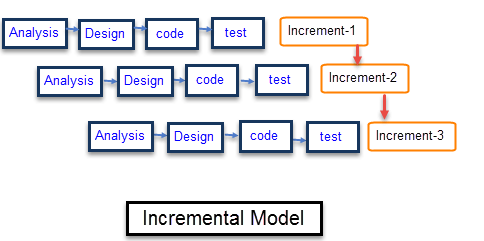
\includegraphics[width=0.9\textwidth]{figs/modelo_incremental.png}
    \caption{Representación del modelo incremental.}
    \label{fig:modelo-incremental}
\end{figure}

\section{Planificaci\'on temporal}
\subsection{Descomposición de tareas por fases}
La planificación se ha dividido en siete bloques principales: \textbf{Inicio, Estado del arte, An\'alisis, Dise\~no, Implementaci\'on, Pruebas} y \textbf{Documentaci\'on}, en concordancia con el modelo incremental utilizado.

\subsubsection*{1. Inicio}
\begin{itemize}
  \item Estudio del problema que resuelve la app
  \item Definición de objetivos del TFG
  \item Planificación inicial del proyecto
\end{itemize}

\subsubsection*{2. Estado del arte}
\begin{itemize}
  \item Revisión de apps similares educativas, con RA y mapas
  \item Estudio de mujeres y sus lugares en Valencia
  \item Estudio de frameworks de RA, mapas y escáneres QR
  \item Selección de tecnologías definitivas (React Native, Django, AFrame)
\end{itemize}

\subsubsection*{3. Análisis}
\begin{itemize}
  \item Definición detallada de requisitos funcionales y no funcionales
  \item Modelado inicial del sistema: navegación y casos de uso
  \item Modelado entidad-relación de la base de datos
  \item Definición de métricas y rutas
\end{itemize}

\subsubsection*{4. Diseño}
\begin{itemize}
  \item Diseño de la arquitectura frontend y backend
  \item Diseño de interfaz móvil y estilo visual
  \item Diseño de pantallas clave: login, listado, mapa, RA, etc.
\end{itemize}

\subsubsection*{5. Implementación backend}
\begin{itemize}
  \item Creación del proyecto Django y configuración Docker
  \item Creación de modelos de datos y migraciones
  \item Implementación de API REST para usuarios, lugares y rutas
  \item Sistema de login y sesiones
  \item Registro de visitas, logros y progreso
\end{itemize}

\subsubsection*{6. Implementación frontend}
\begin{itemize}
  \item Configuración base y navegación
  \item Registro e inicio de sesión de usuarios
  \item Implementación del listado y filtros por ámbito y visitas
  \item Implementación del historial de usuario
  \item Implementación de mapa con geolocalización
  \item Escaneo de QR y navegación a detalle
  \item Sincronización de datos con backend
\end{itemize}

\subsubsection*{7. Implementación de realidad aumentada}
\begin{itemize}
  \item Configuración de AR.js y marcador personalizado
  \item Activación de RA según la ubicación (menos de 1km)
  \item Visualización de modelo 3D y contenido RA educativo
\end{itemize}

\subsubsection*{8. Pruebas y validación}
\begin{itemize}
  \item Pruebas funcionales de cada módulo
  \item Pruebas completas con usuarios externos
  \item Corrección de errores y mejoras detectadas
\end{itemize}

\subsubsection*{9. Documentación}
\begin{itemize}
  \item Redacción progresiva de la memoria (paralela a todo el desarrollo)
  \item Revisión completa, maquetación y anexos finales
\end{itemize}

\subsection{Estimación temporal}
La técnica de estimación utilizada es la media beta de probabilidad. Para cada tarea se ha asignado un tiempo optimista (TO), pesimista (TP) y más probable (TM), y se ha calculado la duración estimada (TE) con la siguiente fórmula:

\begin{center}
$TE = \frac{TO + 4 \cdot TM + TP}{6}$
\end{center}

\begin{table}[H]
\centering
\caption{Estimación por tres valores de las tareas del proyecto}
\begin{tabular}{|l|c|c|c|c|}
\hline
\textbf{Tarea} & \textbf{TO} & \textbf{TP} & \textbf{TM} & \textbf{TE} \\
\hline
Estudio del problema & 1 & 3 & 2 & 2.00 \\
Definición de objetivos & 1 & 2 & 1 & 1.17 \\
Planificación inicial & 1 & 2 & 1 & 1.17 \\
Revisión apps similares & 2 & 4 & 3 & 3.00 \\
Estudio lugares mujeres & 1 & 3 & 2 & 2.00 \\
Frameworks RA y QR & 2 & 4 & 3 & 3.00 \\
Selección tecnologías & 1 & 2 & 1 & 1.17 \\
Requisitos funcionales & 2 & 4 & 3 & 3.00 \\
Casos de uso y navegación & 1 & 3 & 2 & 2.00 \\
Modelo E-R BD & 1 & 3 & 2 & 2.00 \\
Def. métricas y rutas & 1 & 2 & 1 & 1.17 \\
Diseño arquitectura & 2 & 4 & 3 & 3.00 \\
Diseño interfaz visual & 2 & 5 & 3 & 3.17 \\
Pantallas clave & 2 & 4 & 3 & 3.00 \\
Django y Docker & 1 & 3 & 2 & 2.00 \\
Modelos y migraciones & 1 & 3 & 2 & 2.00 \\
API usuarios y lugares & 3 & 5 & 4 & 4.00 \\
Login y sesiones & 1 & 3 & 2 & 2.00 \\
Registro visitas y logros & 1 & 3 & 2 & 2.00 \\
Conf. navegación base & 1 & 3 & 2 & 2.00 \\
Registro e inicio sesión & 1 & 3 & 2 & 2.00 \\
Listado y filtros & 2 & 4 & 3 & 3.00 \\
Historial de usuario & 1 & 3 & 2 & 2.00 \\
Mapa geolocalizado & 2 & 4 & 3 & 3.00 \\
Escaneo QR & 1 & 3 & 2 & 2.00 \\
Sincronización datos & 1 & 3 & 2 & 2.00 \\
Config. AR.js y marcador & 1 & 3 & 2 & 2.00 \\
Desbloqueo por distancia & 1 & 3 & 2 & 2.00 \\
Visualización RA & 2 & 4 & 3 & 3.00 \\
Pruebas funcionales & 2 & 4 & 3 & 3.00 \\
Pruebas con usuarios & 1 & 3 & 2 & 2.00 \\
Corrección errores & 1 & 3 & 2 & 2.00 \\
Redacción progresiva & 4 & 6 & 5 & 5.00 \\
Revisión y entrega final & 2 & 4 & 3 & 3.00 \\
\hline
\textbf{Total estimado} & 73 & 127 & 96 & \textbf{100.00 días} \\
\hline
\end{tabular}
\end{table}

\subsection{Diagrama de Gantt}

Para representar la planificación temporal del proyecto de forma visual, se ha elaborado un diagrama de Gantt utilizando \texttt{Microsoft Project}, teniendo en cuenta las dependencias y la posibilidad de solapar tareas como la documentación progresiva.

\begin{figure}[H]
    \centering
    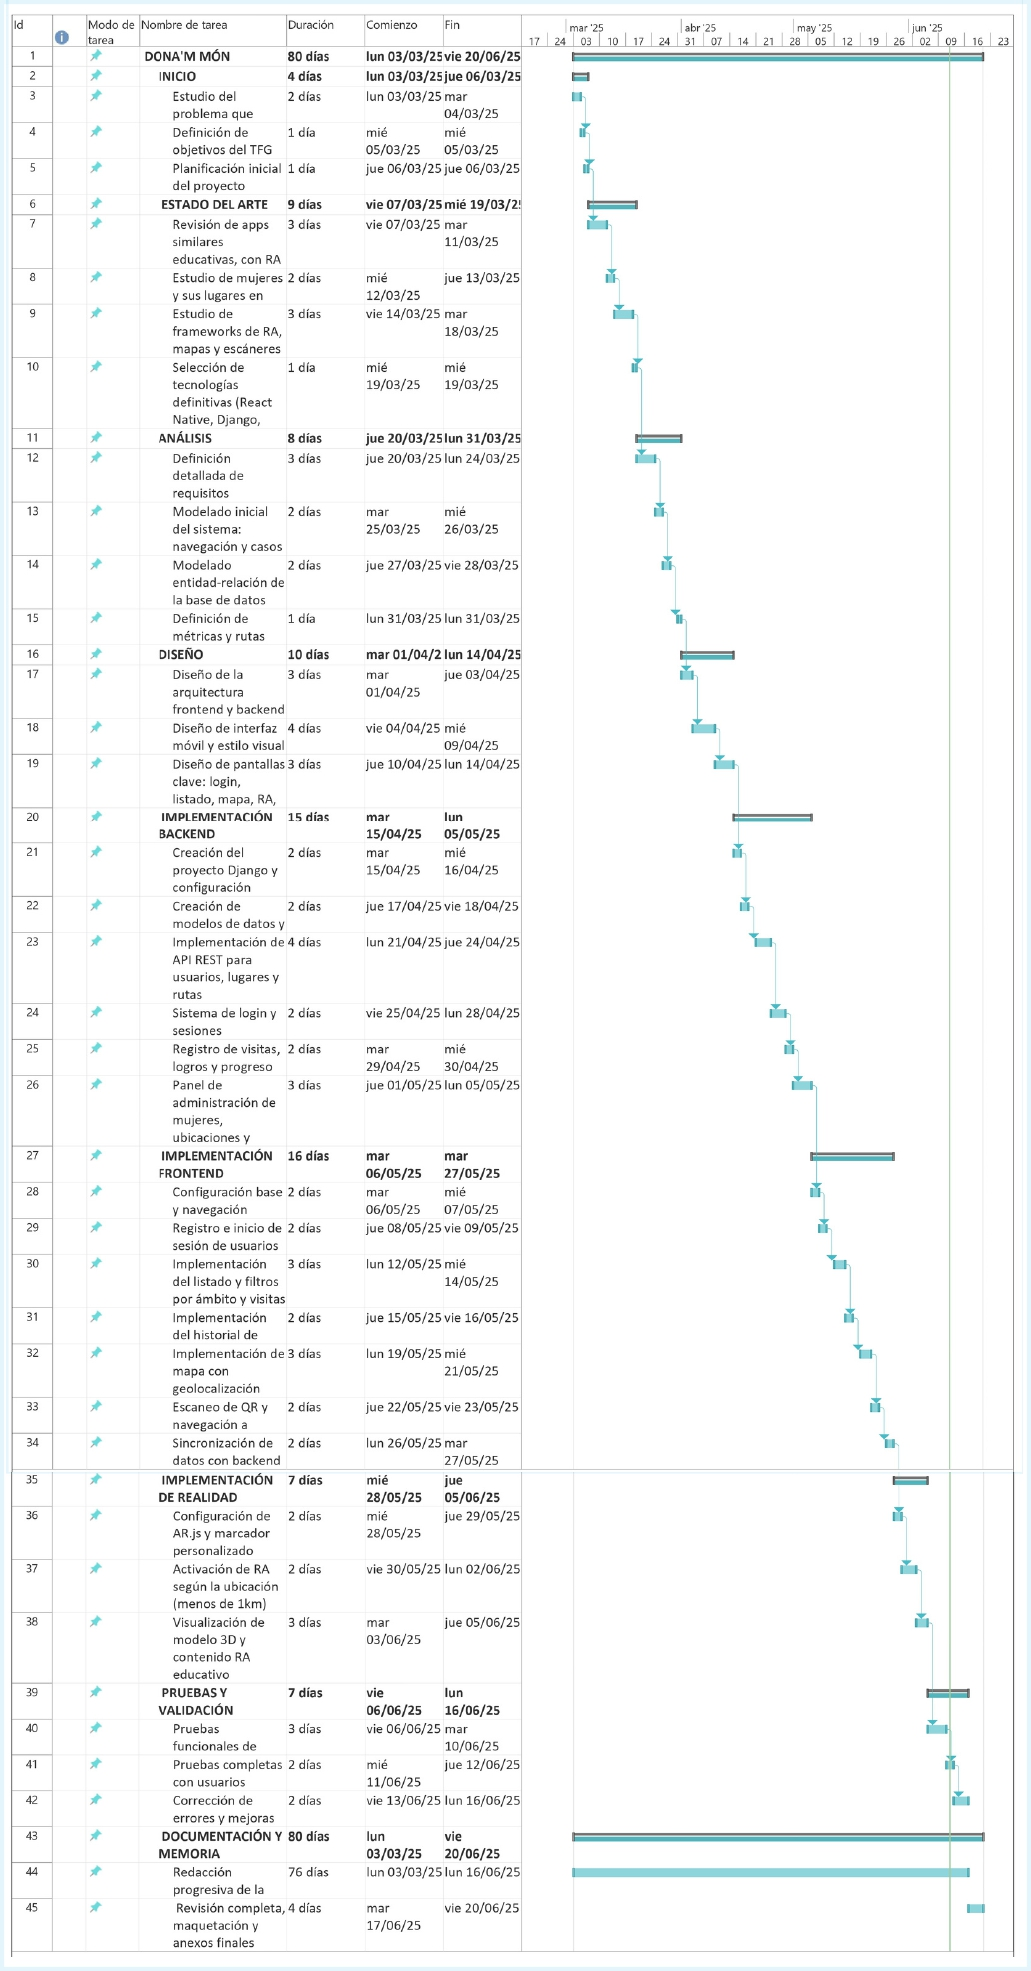
\includegraphics[width=\textwidth,height=0.95\textheight,keepaspectratio]{figs/gantt.jpg}
    \caption{Diagrama de Gantt detallado del proyecto.}
    \label{fig:gantt}
\end{figure} 

A pesar de que la estimación por tres valores del proyecto arroja una duración total de aproximadamente \textbf{100 días} (equivalente a \textbf{800 horas}), el desarrollo real se ha planificado a lo largo de \textbf{80 días laborables} (como puede observarse en el diagrama de Gantt), lo que supone un total de \textbf{640 horas efectivas} de trabajo, distribuidas en jornadas de \textbf{8 horas al día}.

Cabe destacar que:
\begin{itemize}
    \item El proyecto se ha realizado en paralelo con el \textit{Máster en Tecnologías Web, Computación en la Nube y Aplicaciones Móviles}.
    \item Además, durante este periodo se estaban llevando a cabo \textit{prácticas extracurriculares en el Instituto de Robótica y Tecnologías de la Información y la Comunicación (IRTIC)}, donde también se ha avanzado el desarrollo del TFG.
    \item No se ha trabajado durante los fines de semana, por lo que los 80 días corresponden exclusivamente a días laborables.
\end{itemize}

La fecha de inicio del proyecto fue el \textbf{3 de marzo de 2025}, y la fecha de finalización fue el \textbf{20 de junio de 2025}. El proyecto ha sido planificado y ejecutado con el objetivo de ser presentado en la \textbf{primera convocatoria}.
\section{Estimación de costes}

La estimación económica del proyecto se ha realizado distinguiendo entre:
\begin{itemize}
  \item \textbf{Costes directos de personal:} incluyen el salario bruto anual para cada perfil profesional, junto con los costes de Seguridad Social correspondientes (aproximadamente un 30\% adicionales). Se han considerado perfiles distintos (Jefe de Proyecto, Desarrollador Backend, Desarrollador Frontend, Desarrolador de Realidad Tester/QA y Modelador 3D), aunque el proyecto sea llevado a cabo por una sola persona.
  \item \textbf{Costes directos de material:} contemplan licencias, equipos y amortización del hardware y software utilizado.
  \item \textbf{Costes indirectos:} coeficiente adicional del 20\% aplicado sobre el total de los costes directos, para cubrir gastos generales asociados (electricidad, internet, etc.).
\end{itemize}


Este desglose permite dimensionar correctamente los recursos implicados y simular una estructura empresarial, acorde con los requisitos formales del TFG.

\subsection{Costes directos de personal}

Se han obtenido los sueldos medios anuales en España para cada perfil profesional a partir del portal \textit{Glassdoor}~\cite{glassdoorJefeProyecto,glassdoorFrontend,glassdoorBackend,glassdoorTester,glassdoorModelador3D,glassdoorDiseñadr,glassdoorARDeveloper}. A cada salario bruto se le añade un 30\% adicional correspondiente a cotizaciones sociales: contingencias comunes, desempleo, formación y Fogasa.

Se asume una jornada laboral de 8~h/día, 20 días laborables por mes y 11 meses de trabajo al año, siendo 220 días laborales al año. La planificación se basa en 80 días efectivos de trabajo entre el \textbf{3 de marzo y el 20 de junio de 2025}, distribuidos entre los distintos perfiles según su implicación en cada fase.

\begin{table}[H]
\centering
\caption{Perfiles y costes de personal (según cotización SS 2025)}
\begin{tabular}{|l|r|r|r|r|r|}
\hline
\textbf{Perfil} & \textbf{Bruto/año (€)} & \textbf{+31.4\% SS (€)} & \textbf{Total (€)} & \textbf{€/día} & \textbf{€/h} \\
\hline
Jefe de Proyecto        & 40\,500 & 12\,717.00 & 53\,217.00 & 270.92 & 33.87 \\
Desarrollador Frontend  & 40\,500 & 12\,717.00 & 53\,217.00 & 270.92 & 33.87 \\
Desarrollador Backend   & 30\,000 & 9\,420.00  & 39\,420.00 & 200.10 & 25.01 \\
Desarrollador RA        & 23\,000 & 7\,222.00  & 30\,222.00 & 153.68 & 19.21 \\
Tester / QA             & 23\,500 & 7\,379.00  & 30\,879.00 & 156.71 & 19.59 \\
Modelador 3D            & 12\,000 & 3\,768.00  & 15\,768.00 & 79.84  & 9.98  \\
Diseñador gráfico       & 26\,000 & 8\,164.00  & 34\,164.00 & 173.32 & 21.67 \\
\hline
\end{tabular}
\end{table}



\subsection{Asignación temporal por perfil}

Se ha asignado a cada perfil el número estimado de jornadas necesarias para cubrir las tareas planificadas según el cronograma de trabajo. A continuación, se presenta la estimación de coste directo de personal en función de esas jornadas.

\begin{table}[H]
\centering
\caption{Asignación de tareas y costes por perfil}
\begin{tabular}{|l|c|r|p{6.5cm}|r|}
\hline
\textbf{Perfil} & \textbf{Días} & \textbf{€/día} & \textbf{Tareas} & \textbf{Coste (€)} \\
\hline
Jefe de Proyecto & 50 & 270.92 & Estudio inicial, definición de objetivos, planificación, selección de tecnologías, coordinación general & 13,546.00 \\
\hline
Desarrollador Frontend & 16 & 270.92 & Diseño arquitectura frontend, desarrollo UI, navegación, QR, filtros, mapa & 4,334.72 \\
\hline
Desarrollador Backend & 15 & 200.10 & Creación API Django, modelo de datos, autenticación, sincronización backend & 3,001.50 \\
\hline
Desarrollador RA & 7 & 153.68 & Integración AR.js, activación por proximidad, carga de modelos RA & 1,075.76 \\
\hline
Tester / QA & 7 & 156.71 & Pruebas funcionales, pruebas con usuarios, validación y corrección de errores & 1,096.97 \\
\hline
Modelador 3D & 15 & 79.84 & Diseño y preparación de modelos 3D para RA & 1,197.60 \\
\hline
Diseñador gráfico & 20 & 173.32 & Diseño interfaz, estilo visual, iconos y logotipos & 3,466.40 \\
\hline
\end{tabular}
\end{table}

\subsection{Costes directos de material}

Los costes directos de material comprenden los recursos físicos y licencias digitales utilizados durante el desarrollo del proyecto. Para estimar su impacto económico real, se ha calculado la amortización proporcional al tiempo de uso, aplicando la fórmula:

\[
\text{Amortización} = \frac{\text{Precio unidad} \times \text{Días de uso}}{\text{Días de vida útil}}
\]

\begin{table}[H]
\centering
\small
\caption{Elementos utilizados y coste amortizado durante el desarrollo (80 días)}
\resizebox{0.92\textwidth}{!}{%
\begin{tabular}{|l|r|c|c|r|}
\hline
\textbf{Elemento} & \textbf{Precio (€)} & \textbf{Vida útil} & \textbf{Uso (días)} & \textbf{Coste amortizado (€)} \\
\hline
Portátil Asus ROG Strix G15      & 999.00 & 5 años (1825 días)  & 80 & 43.79 \\
iPhone 11                        & 749.00 & 4 años (1460 días)  & 80 & 41.03 \\
Ratón Logitech G203              & 20.99  & 5 años (1825 días)  & 80 & 0.92  \\
Visual Paradigm (mensual)        & 30.00  & 30 días              & 30 & 30.00 \\
Microsoft 365 Business Standard  & 12.50  & 30 días              & 30 & 12.50 \\
Visual Studio Code (profesional) & 45.00  & 365 días             & 80 & 9.86  \\
Docker Pro                       & 99.00  & 365 días             & 80 & 21.70 \\
GitHub Copilot                   & 100.00 & 365 días             & 80 & 21.92 \\
Overleaf Premium                 & 140.00 & 365 días             & 80 & 30.68 \\
\hline
\multicolumn{4}{|r|}{\textbf{Total amortizado}} & \textbf{212.40 €} \\
\hline
\end{tabular}
}%
\end{table}


Cabe destacar que varias de estas herramientas (como Visual Studio Code, Docker o GitHub) disponen de versiones gratuitas o de acceso académico, pero se ha optado por reflejar el coste real de uso profesional para una estimación más realista.

\subsection{Costes indirectos}

Los costes indirectos se han estimado aplicando un coeficiente adicional del 20\% sobre el total de los costes directos (personal y material). Este porcentaje se considera representativo para cubrir gastos generales como el consumo eléctrico, conexión a internet, mantenimiento del equipo, uso de espacios compartidos y otros recursos no imputables directamente al desarrollo del proyecto, pero imprescindibles para su ejecución.

\[
\text{Costes indirectos} = (\text{Costes directos de personal} + \text{Costes directos de material}) \times 0.20
\]

\[
\text{Costes indirectos} = (27\,718.95\ € + 212.40\ €) \times 0.20 = 5\,586.27\ €
\]

\subsection{Coste total del proyecto}

A partir de la suma de los distintos componentes estimados (personal, material e indirectos), se obtiene el coste total simulado del desarrollo del proyecto en un entorno profesional.

\begin{table}[H]
\centering
\caption{Resumen de costes del proyecto}
\begin{tabular}{|l|r|}
\hline
\textbf{Concepto} & \textbf{Coste (€)} \\
\hline
Costes directos de personal & 27\,718.95 \\
Costes directos de material & 212.40 \\
Costes indirectos (20\%) & 5\,586.27 \\
\hline
\textbf{Coste total estimado} & \textbf{33\,517.62} \\
\hline
\end{tabular}
\end{table}

Esta estimación permite cuantificar de forma realista los recursos necesarios para ejecutar un proyecto de características similares en un entorno empresarial. Aunque el trabajo haya sido desarrollado por una única persona, se ha optado por realizar una simulación profesional con perfiles especializados para reflejar adecuadamente la complejidad técnica y el valor añadido del producto final.

\section{Viabilidad del proyecto}

\subsection{Viabilidad económica}

El análisis de costes realizado en la sección anterior ha permitido cuantificar los recursos necesarios para el desarrollo de la aplicación \textit{DONA’m MÓN}. El coste total estimado, que incluye los costes directos de personal (27.718,95~€), costes directos de material (212,40~€) y un 20\% adicional en concepto de costes indirectos (5.586,27~€), asciende a \textbf{33.517,62~€}.

Dado que el proyecto se ha desarrollado sin fines comerciales, el desarrollo ha sido ejecutado por una única persona, utilizando licencias gratuitas, versiones académicas o software de código abierto. Por tanto, los costes no se han asumido en su totalidad. No obstante, se ha realizado una estimación económica completa con el objetivo de evaluar su viabilidad en un contexto profesional o empresarial real, permitiendo así dimensionar correctamente los recursos necesarios en caso de una futura implementación a escala.

El presupuesto puede considerarse razonable si se contempla una posible financiación pública (subvenciones a proyectos culturales, feministas o tecnológicos), financiación universitaria, patrocinio institucional (ayuntamientos, universidades o fundaciones), o apoyo por parte de entidades interesadas en promover la visibilización de mujeres en entornos urbanos y educativos. Además, el impacto social y educativo del proyecto puede justificar su financiación mediante convocatorias de innovación social o género.

\subsection{Viabilidad legal}

Desde el punto de vista legal, el desarrollo de esta aplicación requiere considerar varias cuestiones relevantes:

\begin{itemize}
\item \textbf{Protección de datos personales (RGPD)}: la aplicación permite el registro de usuarios y almacena información relacionada con su ubicación geográfica y su historial de visitas. Por ello, se deberá garantizar el cumplimiento del Reglamento General de Protección de Datos (RGPD), asegurando la obtención del consentimiento explícito del usuario, el almacenamiento seguro de datos y la posibilidad de acceder, rectificar o eliminar la información personal.
\item \textbf{Política de privacidad y condiciones de uso}: será necesario incluir una política clara y accesible que informe al usuario sobre el tratamiento de sus datos, el uso de la geolocalización y la finalidad educativa de la aplicación.

\item \textbf{Derechos de autor y licencias}: todos los modelos 3D, imágenes, textos y recursos utilizados deben contar con licencia libre (Creative Commons, dominio público) o haber sido creados expresamente para el proyecto. En caso contrario, sería necesario solicitar los permisos adecuados.

\item \textbf{Política de uso de servicios externos}: la aplicación hace uso de tecnologías como \textit{WebView} para integrar experiencias de realidad aumentada desarrolladas con A-Frame y AR.js, por lo que se han respetado sus licencias de uso (ambas de código abierto bajo licencia MIT), garantizando la legalidad del uso de estas herramientas dentro del proyecto.
\end{itemize}

No se han identificado restricciones legales insalvables que impidan la realización o publicación de la aplicación. En todo caso, se recomienda aplicar buenas prácticas en el desarrollo seguro, accesible y ético del software.
\section{Análisis de riesgos}

Durante el desarrollo del proyecto \textit{DONA'm MÓN} se han identificado diversos riesgos que pueden afectar negativamente a su cumplimiento en tiempo, coste o calidad. Para su evaluación se ha utilizado un enfoque cualitativo que combina la estimación de la probabilidad de ocurrencia y el impacto en el proyecto, permitiendo establecer niveles de riesgo y su clasificación prioritaria.

\subsection{Principales riesgos identificados}

En la Tabla~\ref{tabla:riesgos-identificados} se recogen los principales riesgos detectados, su probabilidad estimada, el impacto medido en días de retraso potencial, su nivel de riesgo (NR = Probabilidad × Impacto), la clasificación resultante y la fase del proyecto en la que podrían manifestarse.

\begin{table}[H]
\centering
\caption{Principales riesgos identificados}
\label{tabla:riesgos-identificados}
\resizebox{\textwidth}{!}{%
\begin{tabular}{|p{5cm}|c|c|c|c|c|}
\hline
\textbf{Riesgo} & \textbf{Prob. (\%)} & \textbf{Impacto (días)} & \textbf{NR} & \textbf{Clasificación} & \textbf{Fase} \\
\hline
Retrasos en la integración de la RA con React Native & 40 & 8 & 3.20 & Inaceptable & Ejecución \\
Cambios en dependencias externas (Mapas, RA, etc.) & 30 & 5 & 1.50 & Alto & Ejecución \\
Falta de experiencia previa con tecnologías clave & 35 & 6 & 2.10 & Alto & Planificación/Ejecución \\
Definición ambigua del alcance inicial & 25 & 7 & 1.75 & Alto & Inicio \\
Estimaciones optimistas en tareas críticas & 20 & 6 & 1.20 & Moderado & Planificación \\
Problemas legales (datos, localización, RGPD) & 15 & 5 & 0.75 & Moderado & Inicio \\
Baja disponibilidad de recursos y tiempo personal & 30 & 6 & 1.80 & Alto & Ejecución \\
Errores funcionales en fases finales & 10 & 5 & 0.50 & Bajo & Cierre \\
\hline
\end{tabular}
}
\end{table}


A continuación se describen los riesgos con mayor nivel de prioridad:

\begin{enumerate}
  \item \textbf{Definición ambigua del alcance del proyecto:} Un alcance mal delimitado puede derivar en objetivos poco claros y decisiones incorrectas en fases posteriores del desarrollo.

  \textit{Probabilidad: Media — Impacto: Alto — Nivel de riesgo: Inaceptable}

  \item \textbf{Estimaciones temporales y de costes imprecisas:} Una planificación optimista puede provocar desviaciones significativas respecto al cronograma o sobrecostes imprevistos.

  \textit{Probabilidad: Alta — Impacto: Alto — Nivel de riesgo: Inaceptable}

  \item \textbf{Falta de experiencia con tecnologías específicas:} La falta de familiaridad con herramientas clave como AR.js o A-Frame podría ralentizar la implementación de la funcionalidad de realidad aumentada.

  \textit{Probabilidad: Media — Impacto: Alto — Nivel de riesgo: Inaceptable}

  \item \textbf{Retrasos en la ejecución de tareas clave:} La elevada carga de trabajo asumida por una sola persona incrementa la probabilidad de bloqueos o demoras.

  \textit{Probabilidad: Alta — Impacto: Medio — Nivel de riesgo: Alto}

  \item \textbf{Dependencia de recursos externos:} El uso de librerías de terceros (como AR.js, Mapbox, A-Frame) puede verse afectado por cambios inesperados o falta de mantenimiento.

  \textit{Probabilidad: Media — Impacto: Medio — Nivel de riesgo: Medio}

  \item \textbf{Problemas de compatibilidad entre componentes:} La integración entre tecnologías heterogéneas (React Native, Django, AR.js) podría causar errores o conflictos difíciles de prever.

  \textit{Probabilidad: Baja — Impacto: Alto — Nivel de riesgo: Alto}

  \item \textbf{Riesgos legales:} A pesar de que no se almacena información sensible, el tratamiento de datos de geolocalización y el uso de usuarios registrados exige el cumplimiento de la normativa vigente en materia de protección de datos (RGPD).

  \textit{Probabilidad: Baja — Impacto: Medio — Nivel de riesgo: Medio}
\end{enumerate}


\subsection{Matriz de riesgos}

La figura~\ref{fig:matriz-riesgos} muestra la matriz de evaluación de riesgos utilizada, que relaciona la probabilidad de ocurrencia con la magnitud del impacto. Esta herramienta facilita la clasificación de los riesgos y la priorización de acciones preventivas.

\begin{figure}[H]
\centering
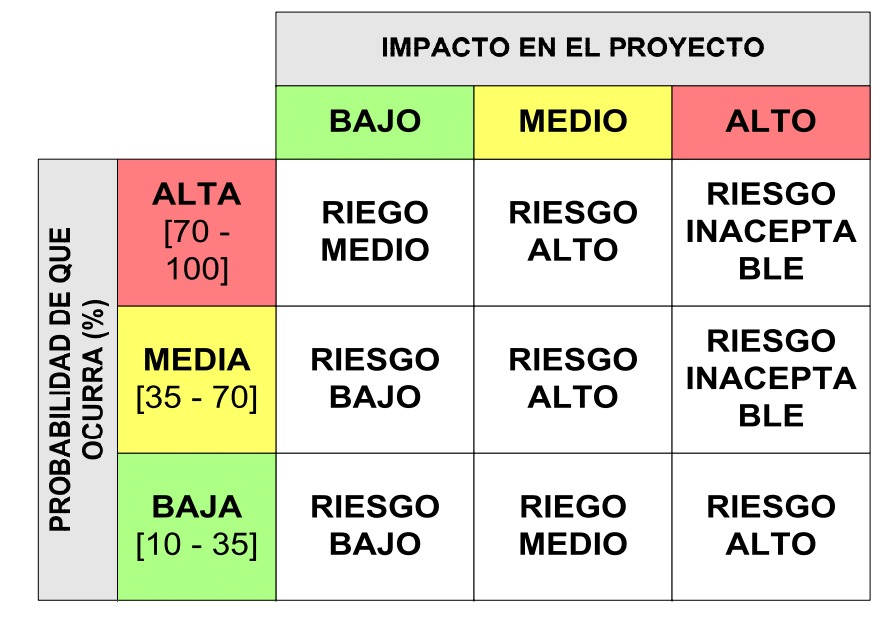
\includegraphics[width=0.65\textwidth]{matriz_riesgos.jpg}
\caption{Matriz de priorización de riesgos utilizada}
\label{fig:matriz-riesgos}
\end{figure}

\subsection{Resumen de evaluación de riesgos}

\begin{table}[H]
\centering
\caption{Resumen cualitativo de evaluación de riesgos}
\label{tabla:resumen-riesgos}
\begin{tabular}{|p{5.5cm}|c|c|c|}
\hline
\textbf{Riesgo} & \textbf{Probabilidad} & \textbf{Impacto} & \textbf{Clasificación} \\
\hline
Definición ambigua del alcance & Media & Alto & Inaceptable \\
Estimaciones temporales imprecisas & Alta & Alto & Inaceptable \\
Falta de experiencia con RA & Media & Alto & Inaceptable \\
Retrasos en tareas clave & Alta & Medio & Alto \\
Dependencia de recursos externos & Media & Medio & Medio \\
Problemas de compatibilidad tecnológica & Baja & Alto & Alto \\
Riesgos legales (RGPD) & Baja & Medio & Medio \\
\hline
\end{tabular}
\end{table}

\subsection{Estrategias de mitigación}

Para minimizar el impacto de los riesgos identificados en el proyecto, se han definido una serie de medidas preventivas orientadas a reducir su probabilidad de ocurrencia o su impacto en caso de materializarse. Estas estrategias se alinean con las buenas prácticas en la gestión de proyectos tecnológicos y tienen carácter proactivo.

\begin{itemize}
  \item \textbf{Definición ambigua del alcance del proyecto:} Se ha trabajado desde el inicio con una delimitación clara del alcance y los objetivos, apoyada por una estructura modular de tareas y entregables. La revisión periódica del cronograma y del backlog funcional permite detectar desviaciones tempranas y corregir posibles ambigüedades.

  \item \textbf{Estimaciones temporales y de costes imprecisas:} La planificación se ha fundamentado en la técnica de estimación por tres valores (optimista, más probable y pesimista), reduciendo la subjetividad y permitiendo incorporar márgenes de seguridad en tareas críticas. Además, se han utilizado referencias de proyectos similares como guía de validación.

  \item \textbf{Falta de experiencia con tecnologías específicas:} Durante la fase de análisis técnico se han realizado pruebas de concepto con las tecnologías clave (AR.js, A-Frame, integración con React Native) para identificar dificultades de forma anticipada. Asimismo, se ha recurrido a documentación oficial, foros especializados y comunidades activas.

  \item \textbf{Retrasos en la ejecución de tareas clave:} Dado que el proyecto es desarrollado por una única persona, se han asignado holguras temporales en tareas críticas y puntos de control semanales para verificar el avance real. El uso de herramientas como Microsoft Project ha permitido detectar desviaciones y replanificar en tiempo real.

  \item \textbf{Dependencia de recursos externos:} Se ha priorizado el uso de herramientas open source con comunidades activas y mantenidas (por ejemplo, AR.js, OpenStreetMap). Además, se han definido posibles alternativas ante fallos o incompatibilidades en recursos externos.

  \item \textbf{Problemas de compatibilidad entre componentes:} La arquitectura del sistema se ha diseñado de forma desacoplada, favoreciendo la integración por medio de interfaces RESTful y estándares abiertos. Esto reduce la posibilidad de conflictos entre tecnologías heterogéneas.

  \item \textbf{Riesgos legales (RGPD):} Aunque no se almacenan datos sensibles, se garantiza el cumplimiento normativo mediante el uso de comunicaciones seguras (HTTPS), el consentimiento del usuario para acceder a la ubicación y la ausencia de almacenamiento persistente de información personal.
\end{itemize}


\subsection{Planes de contingencia}

Se han previsto planes de contingencia específicos para los riesgos más relevantes. Por ejemplo, si se detectan incompatibilidades graves entre tecnologías, se contemplaría el uso de una solución alternativa basada únicamente en mapas interactivos sin RA, manteniendo la funcionalidad básica de exploración de contenidos educativos geolocalizados.



\chapter{Análisis}
% !TEX root = ../ejemplo-memoria.tex
% Contenidos del capítulo.
% Las secciones presentadas son orientativas y no representan
% necesariamente la organización que debe tener este capítulo.


\section*{Introducción}

En este capítulo se realiza el análisis del sistema desde el punto de vista de la Ingeniería del Software. El objetivo es especificar, de manera estructurada y rigurosa, cómo debe comportarse la aplicación y qué funcionalidades debe ofrecer a los distintos tipos de usuarios, siguiendo las metodologías y herramientas propias de la disciplina.

El análisis comienza con la identificación de los roles principales del sistema y las tareas asociadas a cada uno. En el caso de esta aplicación, los roles contemplados son: usuario registrado, usuario no registrado y administrador. Cada uno de ellos dispone de diferentes permisos y accesos a funcionalidades, siendo el administrador quien puede gestionar todos los contenidos y usuarios, mientras que los usuarios registrados acceden a la experiencia completa de la app.

A continuación, se presentan los diagramas de casos de uso, que permiten visualizar de forma global y por rol las interacciones posibles con el sistema. Posteriormente, se detallan los casos de uso más relevantes mediante tablas descriptivas, especificando actores, propósito, precondiciones, postcondiciones y flujos de eventos. Según la naturaleza de la aplicación, también se incluyen diagramas de actividad y de estados para ilustrar los procesos dinámicos y los posibles cambios de estado de los objetos principales.

\section{Diagramas de casos de uso}

A continuación se presentan los diagramas de casos de uso para los diferentes roles del sistema:



\begin{figure}[H]
    \centering
    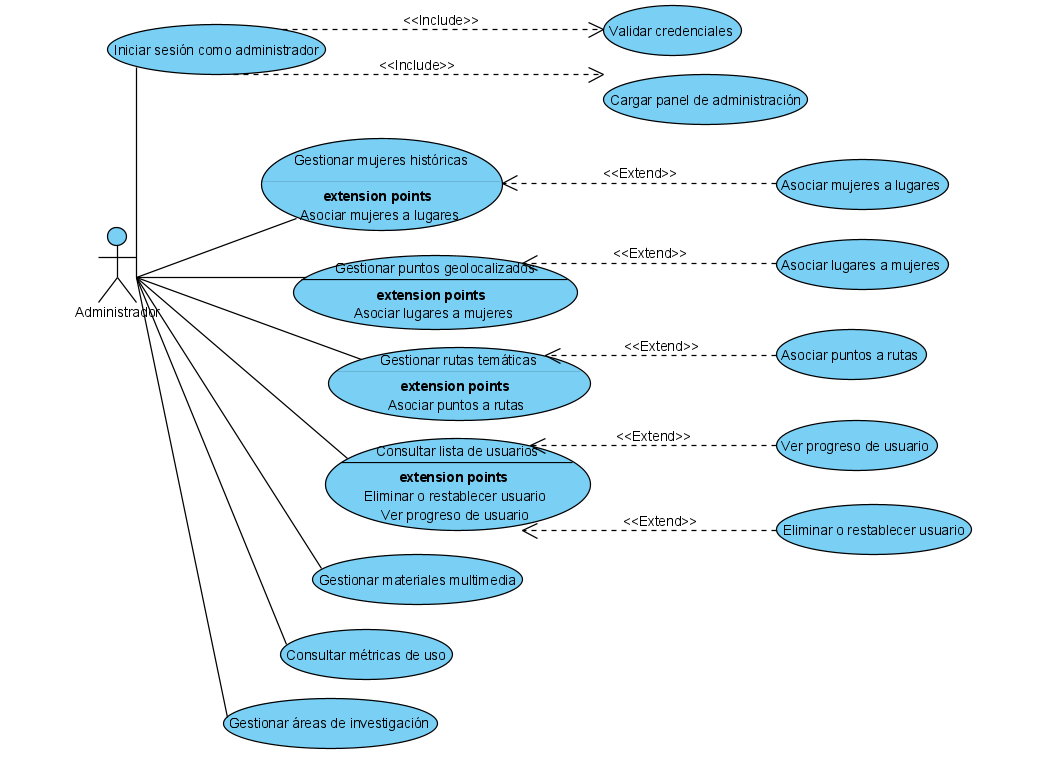
\includegraphics[width=1\textwidth]{figs/diagrama_administrador.png}
    \caption{Diagrama de casos de uso: Administrador}
\end{figure}

\begin{figure}[H]
    \centering
    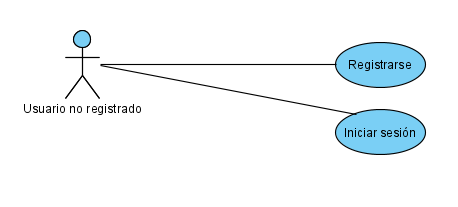
\includegraphics[width=0.8\textwidth]{figs/diagrama_usuario_no_registrado.png}
    \caption{Diagrama de casos de uso: Usuario no registrado}
\end{figure}


\begin{landscape}
    \vfill
    \centering
    \makebox[\paperwidth]{%
        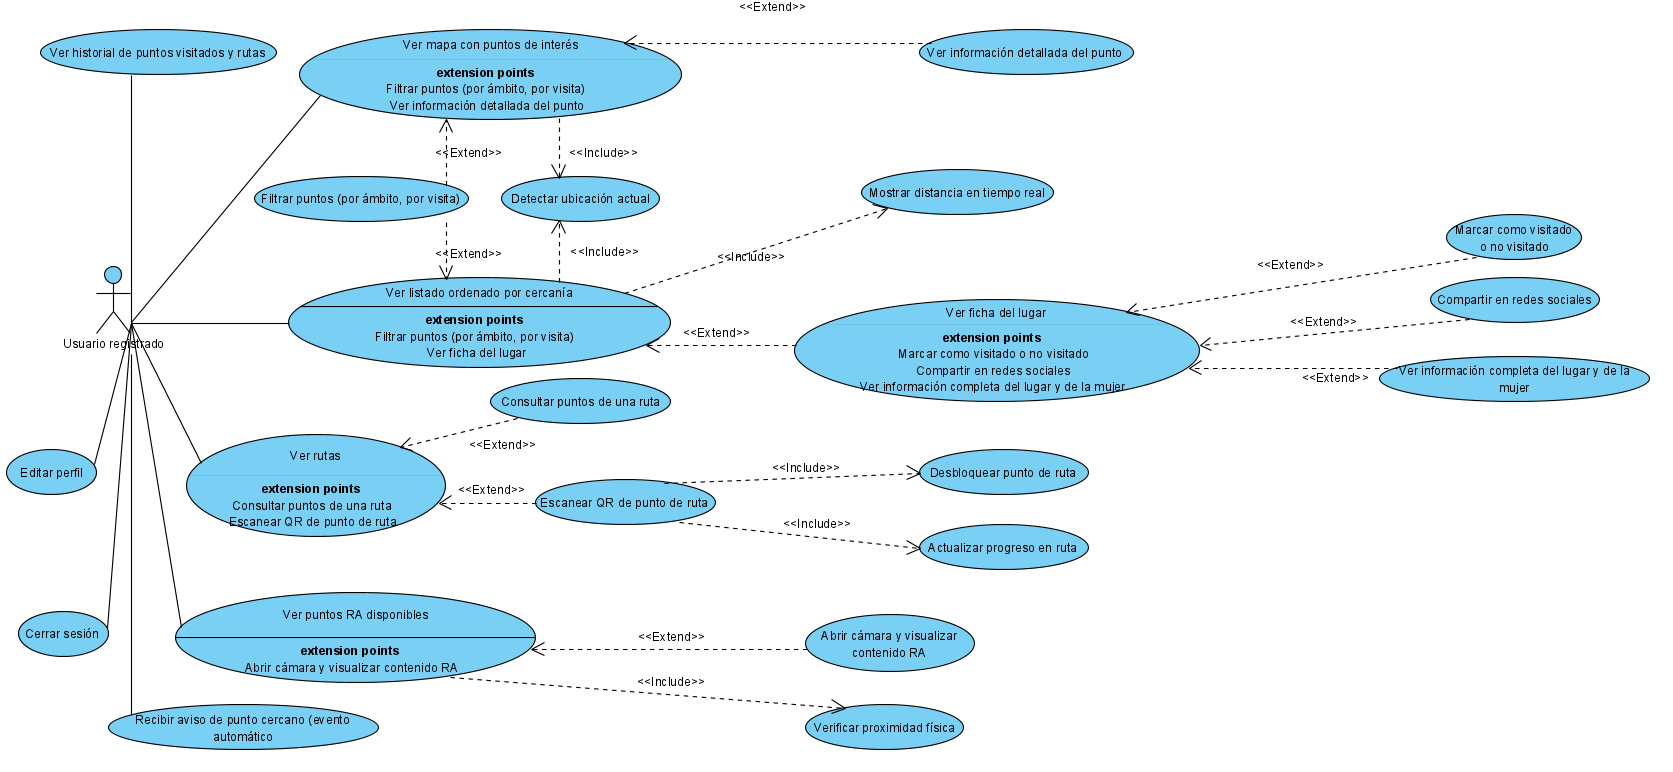
\includegraphics[width=1.2\paperwidth]{figs/diagrama_usuario_registrado.png}
    }
    \par\vspace{1ex}
    \textbf{Figura 4.3: Diagrama de casos de uso: Usuario registrado}
    \vfill
\end{landscape}


\section{Especificación de casos de uso}

A continuación se detallan los casos de uso principales de la aplicación:
\titlespacing{\subsection}{0pt}{*1}{*0.5} % {izq}{antes}{después}
\subsection{Caso de uso 1: Login de usuario}
\captionsetup{skip=0pt}
\begin{table}[H]
\centering
\caption{Caso de uso 1 - Login de usuario}
\begin{tabular}{|p{4.5cm}|p{10.5cm}|}
\hline
\textbf{Nombre del caso de uso} & Login de usuario \\
\hline
\textbf{Actores} & Usuario no registrado (principal), Sistema (secundario) \\
\hline
\textbf{Propósito} & Permitir que el usuario acceda a su cuenta personal mediante correo electrónico y contraseña. \\
\hline
\textbf{Resumen} & Este caso de uso describe el proceso de inicio de sesión mediante credenciales para acceder a las funcionalidades personalizadas de la app. \\
\hline
\textbf{Tipo} & Primario \\
\hline
\textbf{Referencias} & RF23, RF24, RF25 \\
\hline
\textbf{Precondiciones} & El usuario debe tener una cuenta creada previamente. El sistema debe estar operativo y conectado a internet. \\
\hline
\textbf{Postcondiciones} & El usuario inicia sesión correctamente y accede a la pantalla principal de la aplicación, manteniendo la sesión iniciada hasta que decida cerrarla. \\
\hline
\multicolumn{2}{|c|}{\textbf{Flujo de eventos principal}} \\
\hline
\textbf{Actor} & \textbf{Sistema} \\
\hline
1. El usuario abre la aplicación DONA’m MÓN. & \\
\hline
& 2. El sistema muestra la pantalla de login con los campos de email y contraseña. \\
\hline
3. El usuario introduce su email y contraseña. & \\
\hline
& 4. El sistema valida las credenciales en la base de datos. \\
\hline
& 5. Si las credenciales son válidas, se genera un token y se accede a la pantalla principal. \\
\hline
& 6. Si las credenciales no son válidas, se muestra un mensaje de error y se vuelve al paso 2. \\
\hline
\end{tabular}
\end{table}


\subsection{Caso de uso 2: Registro de usuario}

\begin{table}[H]
\centering
\caption{Caso de uso 2 - Registro de usuario}
\begin{tabular}{|p{4.5cm}|p{10.5cm}|}
\hline
\textbf{Nombre del caso de uso} & Registro de usuario \\
\hline
\textbf{Actores} & Usuario no registrado (principal), Sistema (secundario) \\
\hline
\textbf{Propósito} & Permitir que nuevos usuarios creen una cuenta personal mediante un formulario con correo electrónico y contraseña. \\
\hline
\textbf{Resumen} & Este caso de uso describe el proceso por el cual un usuario puede registrarse en la aplicación, aceptando las condiciones de uso y política de privacidad. \\
\hline
\textbf{Tipo} & Primario \\
\hline
\textbf{Referencias} & RF23, RF24, RF25, RNF21, RNF22 \\
\hline
\textbf{Precondiciones} & El sistema debe estar operativo y conectado. El usuario no debe tener una cuenta registrada con ese correo. \\
\hline
\textbf{Postcondiciones} & El usuario queda registrado y accede automáticamente a la pantalla principal con sesión iniciada. \\
\hline
\multicolumn{2}{|c|}{\textbf{Flujo de eventos principal}} \\
\hline
\textbf{Actor} & \textbf{Sistema} \\
\hline
1. El usuario pulsa sobre "Registrarse" en la pantalla de login. & \\
\hline
& 2. El sistema muestra el formulario de registro con los campos de correo, contraseña y checkbox de aceptación legal. \\
\hline
3. El usuario introduce sus datos y acepta la política de privacidad. & \\
\hline
& 4. El sistema verifica que el correo no exista previamente en la base de datos. \\
\hline
& 5. El sistema guarda los datos cifrados y crea la nueva cuenta. \\
\hline
& 6. El sistema genera una sesión automática y redirige a la pantalla principal. \\
\hline
& 7. Si el correo ya existe o hay errores, se muestra un mensaje al usuario. \\
\hline
\end{tabular}
\end{table}
\subsection{Caso de uso 3: Ver mapa con puntos de interés}

\begin{table}[H]
\centering
\caption{Caso de uso 3 - Ver mapa con puntos de interés}
\begin{tabular}{|p{4.5cm}|p{10.5cm}|}
\hline
\textbf{Nombre del caso de uso} & Ver mapa con puntos de interés \\
\hline
\textbf{Actores} & Usuario registrado (principal), Sistema (secundario) \\
\hline
\textbf{Propósito} & Permitir al usuario visualizar un mapa interactivo con los puntos geolocalizados disponibles en la ciudad de Valencia. \\
\hline
\textbf{Resumen} & Este caso de uso describe la carga del mapa, la detección de la ubicación actual, la visualización de los puntos y la posibilidad de aplicar filtros o acceder a la ficha de un punto. \\
\hline
\textbf{Tipo} & Primario \\
\hline
\textbf{Referencias} & RF1, RF2, RF3, RF7, RF8, RF31, RF32 \\
\hline
\textbf{Precondiciones} & El usuario debe haber iniciado sesión y tener permisos de geolocalización habilitados. \\
\hline
\textbf{Postcondiciones} & El usuario ve los puntos en el mapa y puede filtrar, recibir notificaciones o acceder a la ficha de un punto. \\
\hline
\multicolumn{2}{|c|}{\textbf{Flujo de eventos principal}} \\
\hline
\textbf{Actor} & \textbf{Sistema} \\
\hline
1. El usuario accede a la pestaña del mapa. & \\
\hline
& 2. El sistema obtiene la ubicación actual mediante GPS. \\
\hline
& 3. El sistema carga los puntos geolocalizados en el mapa. \\
\hline
2. El usuario activa un filtro por ámbito o estado de visita. & \\
\hline
& 4. El sistema actualiza la visualización del mapa según los filtros. \\
\hline
3. El usuario pulsa sobre un punto del mapa. & \\
\hline
& 5. El sistema abre la ficha detallada del punto seleccionado. \\
\hline
& 6. Si el usuario se aproxima a un punto no visitado, se lanza una notificación. \\
\hline
\end{tabular}
\end{table}

\subsection{Caso de uso 4: Ver listado de puntos ordenado por cercanía}

\begin{table}[H]
\centering
\caption{Caso de uso 4 - Ver listado de puntos ordenado por cercanía}
\begin{tabular}{|p{4.5cm}|p{10.5cm}|}
\hline
\textbf{Nombre del caso de uso} & Ver listado de puntos ordenado por cercanía \\
\hline
\textbf{Actores} & Usuario registrado (principal), Sistema (secundario) \\
\hline
\textbf{Propósito} & Permitir al usuario consultar todos los puntos disponibles organizados automáticamente por distancia desde su ubicación actual. \\
\hline
\textbf{Resumen} & Este caso de uso permite al usuario visualizar un listado de lugares asociados a mujeres históricas, ordenados por cercanía, con filtros por ámbito y estado, y acceso a la ficha de cada uno. \\
\hline
\textbf{Tipo} & Primario \\
\hline
\textbf{Referencias} & RF7, RF8, RF9, RF31, RF32, RF33, RF34, RF35 \\
\hline
\textbf{Precondiciones} & El usuario debe tener sesión iniciada y el GPS activado. \\
\hline
\textbf{Postcondiciones} & El usuario ve una lista actualizada y filtrada de puntos, con acceso a sus fichas. \\
\hline
\multicolumn{2}{|c|}{\textbf{Flujo de eventos principal}} \\
\hline
\textbf{Actor} & \textbf{Sistema} \\
\hline
1. El usuario accede a la pestaña de listado. & \\
\hline
& 2. El sistema detecta la ubicación actual del usuario. \\
\hline
& 3. El sistema obtiene todos los puntos disponibles. \\
\hline
& 4. El sistema calcula y muestra la distancia en tiempo real a cada punto. \\
\hline
& 5. El sistema ordena el listado por cercanía ascendente. \\
\hline
2. El usuario aplica un filtro por ámbito o por estado de visita. & \\
\hline
& 6. El sistema actualiza el listado aplicando los filtros seleccionados. \\
\hline
3. El usuario pulsa sobre un punto del listado. & \\
\hline
& 7. El sistema abre la ficha detallada del punto. \\
\hline
\end{tabular}
\end{table}

\subsection{Caso de uso 5: Ver ficha del lugar}

\begin{table}[H]
\centering
\caption{Caso de uso 1.5 - Ver ficha del lugar}
\begin{tabular}{|p{4.5cm}|p{10.5cm}|}
\hline
\textbf{Nombre del caso de uso} & Ver ficha del lugar \\
\hline
\textbf{Actores} & Usuario registrado (principal), Sistema (secundario) \\
\hline
\textbf{Propósito} & Permitir al usuario visualizar toda la información del lugar y de la figura femenina representada, incluyendo contenido educativo multimedia. \\
\hline
\textbf{Resumen} & Este caso de uso describe el acceso a la ficha completa de un punto, con texto, imágenes, biografía de la mujer, ubicación y la posibilidad de marcar como visitado o compartir por redes sociales. \\
\hline
\textbf{Tipo} & Primario \\
\hline
\textbf{Referencias} & RF4, RF5, RF12, RF13, RF14, RF36 \\
\hline
\textbf{Precondiciones} & El usuario debe haber accedido desde el mapa o listado, seleccionando un punto. \\
\hline
\textbf{Postcondiciones} & El usuario ha consultado la información y puede haber marcado el punto como visitado o compartido el contenido. \\
\hline
\multicolumn{2}{|c|}{\textbf{Flujo de eventos principal}} \\
\hline
\textbf{Actor} & \textbf{Sistema} \\
\hline
1. El usuario pulsa sobre un punto desde el mapa o el listado. & \\
\hline
& 2. El sistema carga los datos completos del lugar y de la mujer histórica asociada. \\
\hline
& 3. El sistema muestra el contenido educativo (texto, imágenes y/o audio). \\
\hline
2. El usuario pulsa “Marcar como visitado”. & \\
\hline
& 4. El sistema actualiza el estado del punto como visitado y lo guarda en el historial. \\
\hline
3. El usuario pulsa “Compartir”. & \\
\hline
& 5. El sistema lanza el menú para compartir el contenido en redes sociales. \\
\hline
\end{tabular}
\end{table}

\subsection{Caso de uso 6: Ver rutas y consultar puntos de una ruta}

\begin{table}[H]
\centering
\caption{Caso de uso 6 - Ver rutas y consultar puntos de una ruta}
\begin{tabular}{|p{4.5cm}|p{10.5cm}|}
\hline
\textbf{Nombre del caso de uso} & Ver rutas y consultar puntos de una ruta \\
\hline
\textbf{Actores} & Usuario registrado (principal), Sistema (secundario) \\
\hline
\textbf{Propósito} & Permitir al usuario visualizar las rutas temáticas disponibles y consultar qué puntos forman parte de cada una. \\
\hline
\textbf{Resumen} & Este caso de uso describe cómo el usuario accede a la lista de rutas temáticas (por ejemplo, mujeres científicas), y cómo puede consultar los puntos que debe desbloquear escaneando su QR correspondiente. \\
\hline
\textbf{Tipo} & Primario \\
\hline
\textbf{Referencias} & RF11, RF37 \\
\hline
\textbf{Precondiciones} & El usuario debe haber iniciado sesión. \\
\hline
\textbf{Postcondiciones} & El usuario ha accedido a la información de una ruta y conoce qué puntos contiene. \\
\hline
\multicolumn{2}{|c|}{\textbf{Flujo de eventos principal}} \\
\hline
\textbf{Actor} & \textbf{Sistema} \\
\hline
1. El usuario accede a la pestaña de rutas. & \\
\hline
& 2. El sistema muestra una lista de rutas temáticas disponibles, con su nombre y descripción. \\
\hline
2. El usuario pulsa sobre una de las rutas. & \\
\hline
& 3. El sistema muestra los puntos geolocalizados que componen esa ruta. \\
\hline
& 4. El sistema indica visualmente cuáles han sido desbloqueados y cuáles no. \\
\hline
\end{tabular}
\end{table}

\subsection{Caso de uso 7: Escanear QR de punto de ruta}

\begin{table}[H]
\centering
\caption{Caso de uso 7 - Escanear QR de punto de ruta}
\begin{tabular}{|p{4.5cm}|p{10.5cm}|}
\hline
\textbf{Nombre del caso de uso} & Escanear QR de punto de ruta \\
\hline
\textbf{Actores} & Usuario registrado (principal), Sistema (secundario) \\
\hline
\textbf{Propósito} & Permitir al usuario desbloquear un punto dentro de una ruta temática mediante el escaneo de un código QR. \\
\hline
\textbf{Resumen} & Este caso de uso permite que el usuario avance en una ruta únicamente si ha escaneado correctamente el QR asociado a un punto. Una vez validado, se actualiza su progreso. \\
\hline
\textbf{Tipo} & Primario \\
\hline
\textbf{Referencias} & RF30, RF38, RF39 \\
\hline
\textbf{Precondiciones} & El usuario debe haber iniciado sesión y tener la cámara habilitada. Debe haber accedido previamente a la ruta. \\
\hline
\textbf{Postcondiciones} & Si el código escaneado es válido, el punto se marca como desbloqueado en la ruta y se actualiza el historial del usuario. \\
\hline
\multicolumn{2}{|c|}{\textbf{Flujo de eventos principal}} \\
\hline
\textbf{Actor} & \textbf{Sistema} \\
\hline
1. El usuario accede a una ruta y pulsa sobre un punto no desbloqueado. & \\
\hline
2. El usuario pulsa el botón "Escanear QR". & \\
\hline
& 3. El sistema abre la cámara y espera a que el usuario enfoque el código QR. \\
\hline
3. El usuario escanea el QR. & \\
\hline
& 4. El sistema valida que el QR corresponde al punto correcto. \\
\hline
& 5. Si es válido, el sistema desbloquea el punto y lo marca como visitado. \\
\hline
& 6. El sistema actualiza el progreso del usuario en esa ruta. \\
\hline
& 7. Si el código QR no es válido, se muestra un mensaje de error. \\
\hline
\end{tabular}
\end{table}

\subsection{Caso de uso 8: Ver puntos RA disponibles}

\begin{table}[H]
\centering
\caption{Caso de uso 8 - Ver puntos RA disponibles}
\begin{tabular}{|p{4.5cm}|p{10.5cm}|}
\hline
\textbf{Nombre del caso de uso} & Ver puntos RA disponibles \\
\hline
\textbf{Actores} & Usuario registrado (principal), Sistema (secundario) \\
\hline
\textbf{Propósito} & Mostrar al usuario solo los puntos que tienen contenido de realidad aumentada disponible y que están dentro del radio permitido. \\
\hline
\textbf{Resumen} & Este caso de uso describe cómo el sistema filtra automáticamente los puntos que disponen de RA y están dentro del rango de distancia del usuario para que puedan visualizarse. \\
\hline
\textbf{Tipo} & Primario \\
\hline
\textbf{Referencias} & RF40, RF41 \\
\hline
\textbf{Precondiciones} & El usuario debe tener sesión iniciada, el GPS activado y conexión a internet. \\
\hline
\textbf{Postcondiciones} & El usuario visualiza un listado de puntos RA disponibles que puede seleccionar para abrir el contenido RA. \\
\hline
\multicolumn{2}{|c|}{\textbf{Flujo de eventos principal}} \\
\hline
\textbf{Actor} & \textbf{Sistema} \\
\hline
1. El usuario accede a la pestaña de RA. & \\
\hline
& 2. El sistema detecta la ubicación actual del usuario. \\
\hline
& 3. El sistema filtra los puntos con contenido RA. \\
\hline
& 4. El sistema calcula qué puntos RA están dentro del radio permitido. \\
\hline
& 5. El sistema muestra el listado de puntos RA disponibles cercanos. \\
\hline
\end{tabular}
\end{table}

\subsection{Caso de uso 1.9: Visualizar contenido RA}

\begin{table}[H]
\centering
\caption{Caso de uso 9 - Visualizar contenido RA}
\begin{tabular}{|p{4.5cm}|p{10.5cm}|}
\hline
\textbf{Nombre del caso de uso} & Visualizar contenido RA \\
\hline
\textbf{Actores} & Usuario registrado (principal), Sistema (secundario) \\
\hline
\textbf{Propósito} & Permitir al usuario visualizar los modelos 3D o elementos interactivos en RA sobre el entorno real desde la cámara del dispositivo. \\
\hline
\textbf{Resumen} & Este caso de uso describe el proceso de abrir la cámara desde un punto RA cercano y mostrar el contenido de realidad aumentada asociado, como un modelo 3D vinculado a una mujer histórica. \\
\hline
\textbf{Tipo} & Primario \\
\hline
\textbf{Referencias} & RF41 \\
\hline
\textbf{Precondiciones} & El usuario debe haber accedido a la pestaña RA, seleccionado un punto válido y concedido permiso de cámara. \\
\hline
\textbf{Postcondiciones} & El usuario visualiza el contenido RA correctamente alineado sobre el marcador o la ubicación. \\
\hline
\multicolumn{2}{|c|}{\textbf{Flujo de eventos principal}} \\
\hline
\textbf{Actor} & \textbf{Sistema} \\
\hline
1. El usuario pulsa sobre un punto RA disponible. & \\
\hline
& 2. El sistema solicita permisos para acceder a la cámara. \\
\hline
& 3. El sistema abre la cámara del dispositivo. \\
\hline
& 4. El sistema detecta la ubicación o el marcador visual. \\
\hline
& 5. El sistema carga el modelo RA correspondiente (imagen, animación o 3D). \\
\hline
& 6. El sistema muestra el modelo RA en tiempo real superpuesto al entorno. \\
\hline
\end{tabular}
\end{table}

\subsection{Caso de uso 10: Editar perfil de usuario}

\begin{table}[H]
\centering
\caption{Caso de uso 10 - Editar datos del perfil}
\begin{tabular}{|p{4.5cm}|p{10.5cm}|}
\hline
\textbf{Nombre del caso de uso} & Editar datos del perfil \\
\hline
\textbf{Actores} & Usuario registrado (principal), Sistema (secundario) \\
\hline
\textbf{Propósito} & Permitir al usuario modificar sus datos personales como nombre, correo o contraseña desde la sección de perfil. \\
\hline
\textbf{Resumen} & Este caso de uso describe cómo un usuario puede acceder a su perfil, modificar la información personal y guardar los cambios, los cuales se actualizan en la base de datos. \\
\hline
\textbf{Tipo} & Primario \\
\hline
\textbf{Referencias} & RF26, RF42 \\
\hline
\textbf{Precondiciones} & El usuario debe tener sesión iniciada. Debe estar en la sección de perfil. \\
\hline
\textbf{Postcondiciones} & Los datos del perfil del usuario quedan actualizados correctamente en el sistema. \\
\hline
\multicolumn{2}{|c|}{\textbf{Flujo de eventos principal}} \\
\hline
\textbf{Actor} & \textbf{Sistema} \\
\hline
1. El usuario accede a la pestaña de perfil. & \\
\hline
2. El usuario pulsa el botón "Editar perfil". & \\
\hline
3. El usuario modifica los campos deseados. & \\
\hline
4. El usuario pulsa el botón "Guardar cambios". & \\
\hline
& 5. El sistema valida los nuevos datos. \\
\hline
& 6. El sistema actualiza los datos del usuario en la base de datos. \\
\hline
& 7. El sistema muestra un mensaje de confirmación. \\
\hline
\end{tabular}
\end{table}

\subsection{Caso de uso 11: Ver historial de lugares visitados y rutas completadas}

\begin{table}[H]
\centering
\caption{Caso de uso 11 - Ver historial de lugares visitados y rutas completadas}
\begin{tabular}{|p{4.5cm}|p{10.5cm}|}
\hline
\textbf{Nombre del caso de uso} & Ver historial de lugares visitados y rutas completadas \\
\hline
\textbf{Actores} & Usuario registrado (principal), Sistema (secundario) \\
\hline
\textbf{Propósito} & Permitir al usuario consultar qué puntos ha visitado y qué rutas ha completado, con su respectiva fecha y hora. \\
\hline
\textbf{Resumen} & Este caso de uso permite al usuario ver un resumen personalizado de su progreso en la app, incluyendo puntos visitados, rutas completadas y fechas correspondientes. \\
\hline
\textbf{Tipo} & Primario \\
\hline
\textbf{Referencias} & RF14, RF42, F43, F44 \\
\hline
\textbf{Precondiciones} & El usuario debe tener sesión iniciada. \\
\hline
\textbf{Postcondiciones} & El usuario visualiza su historial actualizado, sin modificar ningún dato. \\
\hline
\multicolumn{2}{|c|}{\textbf{Flujo de eventos principal}} \\
\hline
\textbf{Actor} & \textbf{Sistema} \\
\hline
1. El usuario accede a la pestaña de perfil. & \\
\hline
2. El usuario pulsa sobre “Historial de visitas y rutas”. & \\
\hline
& 3. El sistema recupera los datos del historial del usuario desde la base de datos. \\
\hline
& 4. El sistema muestra la lista de puntos visitados con fecha y hora. \\
\hline
& 5. El sistema muestra también las rutas completadas por el usuario. \\
\hline
\end{tabular}
\end{table}


\subsection{Caso de uso 12: Cerrar sesión}

\begin{table}[H]
\centering
\caption{Caso de uso 12 - Cerrar sesión}
\begin{tabular}{|p{4.5cm}|p{10.5cm}|}
\hline
\textbf{Nombre del caso de uso} & Cerrar sesión \\
\hline
\textbf{Actores} & Usuario registrado (principal), Sistema (secundario) \\
\hline
\textbf{Propósito} & Permitir al usuario finalizar su sesión actual y cerrar su acceso a la app hasta el próximo inicio de sesión. \\
\hline
\textbf{Resumen} & Este caso de uso describe cómo el usuario puede cerrar manualmente su sesión desde la sección de perfil, eliminando su token de acceso y volviendo a la pantalla de login. \\
\hline
\textbf{Tipo} & Primario \\
\hline
\textbf{Referencias} & RF25, RF42 \\
\hline
\textbf{Precondiciones} & El usuario debe tener sesión iniciada. \\
\hline
\textbf{Postcondiciones} & La sesión se cierra y el usuario vuelve a la pantalla de login. \\
\hline
\multicolumn{2}{|c|}{\textbf{Flujo de eventos principal}} \\
\hline
\textbf{Actor} & \textbf{Sistema} \\
\hline
1. El usuario accede a la pestaña de perfil. & \\
\hline
2. El usuario pulsa el botón “Cerrar sesión”. & \\
\hline
& 3. El sistema elimina el token de autenticación almacenado. \\
\hline
& 4. El sistema redirige al usuario a la pantalla de login. \\
\hline
\end{tabular}
\end{table}


\subsection{Caso de uso 13: Iniciar sesión como administrador}

\begin{table}[H]
\centering
\caption{Caso de uso 13 - Iniciar sesión como administrador}
\begin{tabular}{|p{4.5cm}|p{10.5cm}|}
\hline
\textbf{Nombre del caso de uso} & Iniciar sesión como administrador \\
\hline
\textbf{Actores} & Administrador (principal), Sistema (secundario) \\
\hline
\textbf{Propósito} & Permitir al administrador acceder al panel de administración web mediante autenticación segura. \\
\hline
\textbf{Resumen} & El administrador introduce sus credenciales (usuario y contraseña) en la pantalla de login del panel de administración. El sistema valida los datos y, si son correctos, permite el acceso a las funcionalidades administrativas. \\
\hline
\textbf{Tipo} & Primario \\
\hline
\textbf{Referencias} & RF16, F20, RNF19 \\
\hline
\textbf{Precondiciones} & El administrador debe estar registrado en el sistema y disponer de credenciales válidas. \\
\hline
\textbf{Postcondiciones} & El administrador accede al panel de administración con los permisos correspondientes. \\
\hline
\multicolumn{2}{|c|}{\textbf{Flujo de eventos principal}} \\
\hline
\textbf{Actor} & \textbf{Sistema} \\
\hline
El administrador accede a la URL del panel de administración. & \\
\hline
El administrador introduce su usuario y contraseña. & \\
\hline
El administrador pulsa el botón de “Iniciar sesión”. & \\
\hline
& 4. El sistema valida las credenciales introducidas. \\
\hline
& 5. Si las credenciales son correctas, el sistema carga el panel de administración. \\
\hline
& 6. Si las credenciales son incorrectas, el sistema muestra un mensaje de error. \\
\hline
\end{tabular}
\end{table}

\subsection{Caso de uso 14: Gestionar mujeres históricas}

\begin{table}[H]
\centering
\caption{Caso de uso 14 - Gestionar mujeres históricas}
\begin{tabular}{|p{4.5cm}|p{10.5cm}|}
\hline
\textbf{Nombre del caso de uso} & Gestionar mujeres históricas \\
\hline
\textbf{Actores} & Administrador (principal), Sistema (secundario) \\
\hline
\textbf{Propósito} & Permitir al administrador crear, editar o eliminar figuras históricas femeninas dentro del sistema. \\
\hline
\textbf{Resumen} & Este caso de uso describe las acciones que puede realizar el administrador para mantener actualizada la base de datos de mujeres históricas: crear nuevas entradas, modificar datos existentes, o eliminarlas. Cada mujer puede estar asociada a uno o varios lugares geolocalizados. \\
\hline
\textbf{Tipo} & Primario \\
\hline
\textbf{Referencias} & RF17, RF18, F21, F22, F24 \\
\hline
\textbf{Precondiciones} & El administrador debe haber iniciado sesión correctamente en el panel de administración. \\
\hline
\textbf{Postcondiciones} & Se actualiza la base de datos de figuras históricas femeninas según las acciones realizadas. \\
\hline
\multicolumn{2}{|c|}{\textbf{Flujo de eventos principal}} \\
\hline
\textbf{Actor} & \textbf{Sistema} \\
\hline
1. El administrador accede a la sección “Mujeres históricas” del panel. & \\
\hline
2. El administrador pulsa sobre “Añadir mujer”, “Editar” o “Eliminar”. & \\
\hline
3. El administrador introduce o modifica datos como nombre, biografía, fechas, y áreas de investigación. & \\
\hline
& 4. El sistema valida los campos requeridos. \\
\hline
& 5. El sistema guarda los datos nuevos o actualizados en la base de datos. \\
\hline
& 6. Si se ha eliminado una figura, se borran también sus asociaciones con puntos. \\
\hline
& 7. El sistema muestra un mensaje de confirmación de los cambios. \\
\hline
\end{tabular}
\end{table}

\subsection{Caso de uso 15: Gestionar puntos geolocalizados}

\begin{table}[H]
\centering
\caption{Caso de uso 15 - Gestionar puntos geolocalizados}
\begin{tabular}{|p{4.5cm}|p{10.5cm}|}
\hline
\textbf{Nombre del caso de uso} & Gestionar puntos geolocalizados \\
\hline
\textbf{Actores} & Administrador (principal), Sistema (secundario) \\
\hline
\textbf{Propósito} & Permitir al administrador crear, editar o eliminar lugares geolocalizados y asociarlos a mujeres históricas. \\
\hline
\textbf{Resumen} & El administrador puede mantener actualizada la base de datos de lugares: crear nuevos puntos, modificar su información (nombre, descripción, ubicación, foto), o eliminarlos. Cada lugar puede estar vinculado a una mujer histórica. \\
\hline
\textbf{Tipo} & Primario \\
\hline
\textbf{Referencias} & RF17, RF18, F22, F24 \\
\hline
\textbf{Precondiciones} & El administrador debe haber iniciado sesión correctamente en el panel de administración. \\
\hline
\textbf{Postcondiciones} & Se actualiza la base de datos de lugares y sus asociaciones con mujeres históricas. \\
\hline
\multicolumn{2}{|c|}{\textbf{Flujo de eventos principal}} \\
\hline
\textbf{Actor} & \textbf{Sistema} \\
\hline
1. El administrador accede a la sección “Lugares” del panel. & \\
\hline
2. El administrador pulsa sobre “Añadir lugar”, “Editar” o “Eliminar”. & \\
\hline
3. El administrador introduce o modifica datos como nombre, descripción, ubicación, foto y mujer asociada. & \\
\hline
& 4. El sistema valida los campos requeridos. \\
\hline
& 5. El sistema guarda los datos nuevos o actualizados en la base de datos. \\
\hline
& 6. Si se elimina un lugar, se eliminan también sus asociaciones. \\
\hline
& 7. El sistema muestra un mensaje de confirmación de los cambios. \\
\hline
\end{tabular}
\end{table}

\subsection{Caso de uso 16: Gestionar rutas temáticas}

\begin{table}[H]
\centering
\caption{Caso de uso 16 - Gestionar rutas temáticas}
\begin{tabular}{|p{4.5cm}|p{10.5cm}|}
\hline
\textbf{Nombre del caso de uso} & Gestionar rutas temáticas \\
\hline
\textbf{Actores} & Administrador (principal), Sistema (secundario) \\
\hline
\textbf{Propósito} & Permitir al administrador crear, editar o eliminar rutas temáticas y asociar puntos a cada ruta. \\
\hline
\textbf{Resumen} & El administrador puede definir rutas temáticas, asignarles nombre y descripción, y asociarles puntos geolocalizados. Puede modificar o eliminar rutas existentes. \\
\hline
\textbf{Tipo} & Primario \\
\hline
\textbf{Referencias} & RF11, RF18b, F24b, F33, F34 \\
\hline
\textbf{Precondiciones} & El administrador debe haber iniciado sesión correctamente en el panel de administración. \\
\hline
\textbf{Postcondiciones} & Se actualiza la base de datos de rutas temáticas y sus asociaciones con puntos. \\
\hline
\multicolumn{2}{|c|}{\textbf{Flujo de eventos principal}} \\
\hline
\textbf{Actor} & \textbf{Sistema} \\
\hline
1. El administrador accede a la sección “Rutas temáticas” del panel. & \\
\hline
2. El administrador pulsa sobre “Añadir ruta”, “Editar” o “Eliminar”. & \\
\hline
3. El administrador introduce o modifica datos como nombre, descripción y puntos asociados. & \\
\hline
& 4. El sistema valida los campos requeridos. \\
\hline
& 5. El sistema guarda los datos nuevos o actualizados en la base de datos. \\
\hline
& 6. Si se elimina una ruta, se eliminan también sus asociaciones. \\
\hline
& 7. El sistema muestra un mensaje de confirmación de los cambios. \\
\hline
\end{tabular}
\end{table}

\subsection{Caso de uso 17: Consultar lista de usuarios}

\begin{table}[H]
\centering
\caption{Caso de uso 17 - Consultar lista de usuarios}
\begin{tabular}{|p{4.5cm}|p{10.5cm}|}
\hline
\textbf{Nombre del caso de uso} & Consultar lista de usuarios \\
\hline
\textbf{Actores} & Administrador (principal), Sistema (secundario) \\
\hline
\textbf{Propósito} & Permitir al administrador visualizar la lista de usuarios registrados, su progreso y gestionar sus cuentas. \\
\hline
\textbf{Resumen} & El administrador puede ver todos los usuarios registrados, consultar su progreso (puntos visitados, logros), y eliminar o restablecer cuentas si es necesario. \\
\hline
\textbf{Tipo} & Primario \\
\hline
\textbf{Referencias} & RF27, RF28, RF29, F25, F26, F27 \\
\hline
\textbf{Precondiciones} & El administrador debe haber iniciado sesión correctamente en el panel de administración. \\
\hline
\textbf{Postcondiciones} & Se actualiza la base de datos de usuarios si se elimina o restablece alguna cuenta. \\
\hline
\multicolumn{2}{|c|}{\textbf{Flujo de eventos principal}} \\
\hline
\textbf{Actor} & \textbf{Sistema} \\
\hline
1. El administrador accede a la sección “Usuarios” del panel. & \\
\hline
2. El administrador selecciona un usuario para ver su perfil y progreso. & \\
\hline
3. El administrador puede eliminar o restablecer la cuenta del usuario. & \\
\hline
& 4. El sistema muestra la información del usuario y su progreso. \\
\hline
& 5. Si se elimina o restablece, el sistema actualiza la base de datos y muestra confirmación. \\
\hline
\end{tabular}
\end{table}

\subsection{Caso de uso 18: Gestionar materiales multimedia}

\begin{table}[H]
\centering
\caption{Caso de uso 18 - Gestionar materiales multimedia}
\begin{tabular}{|p{4.5cm}|p{10.5cm}|}
\hline
\textbf{Nombre del caso de uso} & Gestionar materiales multimedia \\
\hline
\textbf{Actores} & Administrador (principal), Sistema (secundario) \\
\hline
\textbf{Propósito} & Permitir al administrador importar, editar o eliminar imágenes, vídeos y modelos 3D asociados a mujeres o lugares. \\
\hline
\textbf{Resumen} & El administrador puede subir, modificar o eliminar archivos multimedia que se mostrarán en la app, asegurando que el contenido esté actualizado y sea relevante. \\
\hline
\textbf{Tipo} & Primario \\
\hline
\textbf{Referencias} & RF18, F23, F24 \\
\hline
\textbf{Precondiciones} & El administrador debe haber iniciado sesión correctamente en el panel de administración. \\
\hline
\textbf{Postcondiciones} & Se actualiza la base de datos y el repositorio de archivos multimedia. \\
\hline
\multicolumn{2}{|c|}{\textbf{Flujo de eventos principal}} \\
\hline
\textbf{Actor} & \textbf{Sistema} \\
\hline
1. El administrador accede a la sección de gestión multimedia. & \\
\hline
2. El administrador selecciona “Añadir”, “Editar” o “Eliminar” un archivo multimedia. & \\
\hline
3. El administrador sube o modifica el archivo y lo asocia a una mujer o lugar. & \\
\hline
& 4. El sistema valida el formato y tamaño del archivo. \\
\hline
& 5. El sistema guarda o elimina el archivo y actualiza la base de datos. \\
\hline
& 6. El sistema muestra un mensaje de confirmación de los cambios. \\
\hline
\end{tabular}
\end{table}

\subsection{Caso de uso 19: Consultar métricas de uso}

\begin{table}[H]
\centering
\caption{Caso de uso 19 - Consultar métricas de uso}
\begin{tabular}{|p{4.5cm}|p{10.5cm}|}
\hline
\textbf{Nombre del caso de uso} & Consultar métricas de uso \\
\hline
\textbf{Actores} & Administrador (principal), Sistema (secundario) \\
\hline
\textbf{Propósito} & Permitir al administrador visualizar estadísticas y métricas sobre el uso de la aplicación. \\
\hline
\textbf{Resumen} & El administrador puede consultar datos como puntos más visitados, número de usuarios activos, rutas más populares, etc., para tomar decisiones informadas sobre el contenido y la gestión. \\
\hline
\textbf{Tipo} & Primario \\
\hline
\textbf{Referencias} & RF18c, F24c, F28 \\
\hline
\textbf{Precondiciones} & El administrador debe haber iniciado sesión correctamente en el panel de administración. \\
\hline
\textbf{Postcondiciones} & No aplica (consulta de información). \\
\hline
\multicolumn{2}{|c|}{\textbf{Flujo de eventos principal}} \\
\hline
\textbf{Actor} & \textbf{Sistema} \\
\hline
1. El administrador accede a la sección de métricas del panel. & \\
\hline
2. El administrador selecciona el tipo de métrica o informe a consultar. & \\
\hline
& 3. El sistema muestra los datos solicitados en pantalla. \\
\hline
\end{tabular}
\end{table}

\subsection{Caso de uso 20: Gestionar áreas de investigación}

\begin{table}[H]
\centering
\caption{Caso de uso 20 - Gestionar áreas de investigación}
\begin{tabular}{|p{4.5cm}|p{10.5cm}|}
\hline
\textbf{Nombre del caso de uso} & Gestionar áreas de investigación \\
\hline
\textbf{Actores} & Administrador (principal), Sistema (secundario) \\
\hline
\textbf{Propósito} & Permitir al administrador crear, editar o eliminar áreas de investigación asociadas a mujeres históricas. \\
\hline
\textbf{Resumen} & El administrador puede mantener actualizada la lista de áreas de investigación, que luego pueden asociarse a las mujeres históricas para facilitar la búsqueda y filtrado en la app. \\
\hline
\textbf{Tipo} & Primario \\
\hline
\textbf{Referencias} & RF18b, F24b \\
\hline
\textbf{Precondiciones} & El administrador debe haber iniciado sesión correctamente en el panel de administración. \\
\hline
\textbf{Postcondiciones} & Se actualiza la base de datos de áreas de investigación. \\
\hline
\multicolumn{2}{|c|}{\textbf{Flujo de eventos principal}} \\
\hline
\textbf{Actor} & \textbf{Sistema} \\
\hline
1. El administrador accede a la sección de áreas de investigación. & \\
\hline
2. El administrador pulsa sobre “Añadir”, “Editar” o “Eliminar” área. & \\
\hline
3. El administrador introduce o modifica el nombre del área. & \\
\hline
& 4. El sistema valida el campo requerido. \\
\hline
& 5. El sistema guarda o elimina el área en la base de datos. \\
\hline
& 6. El sistema muestra un mensaje de confirmación de los cambios. \\
\hline
\end{tabular}
\end{table}

\section{Diagramas de Actividad}


Los diagramas de actividad son una herramienta utilizada en el modelado de procesos y flujos de trabajo dentro de un sistema. Permiten representar gráficamente la secuencia de actividades, decisiones y flujos alternativos que pueden ocurrir durante la ejecución de un proceso. Son especialmente útiles para visualizar el comportamiento dinámico de un sistema y entender cómo interactúan los distintos componentes o usuarios.

A continuación se muestra un ejemplo de diagrama de actividad correspondiente al flujo de registro e inicio de sesión de usuarios:

\begin{figure}[H]
    \centering
    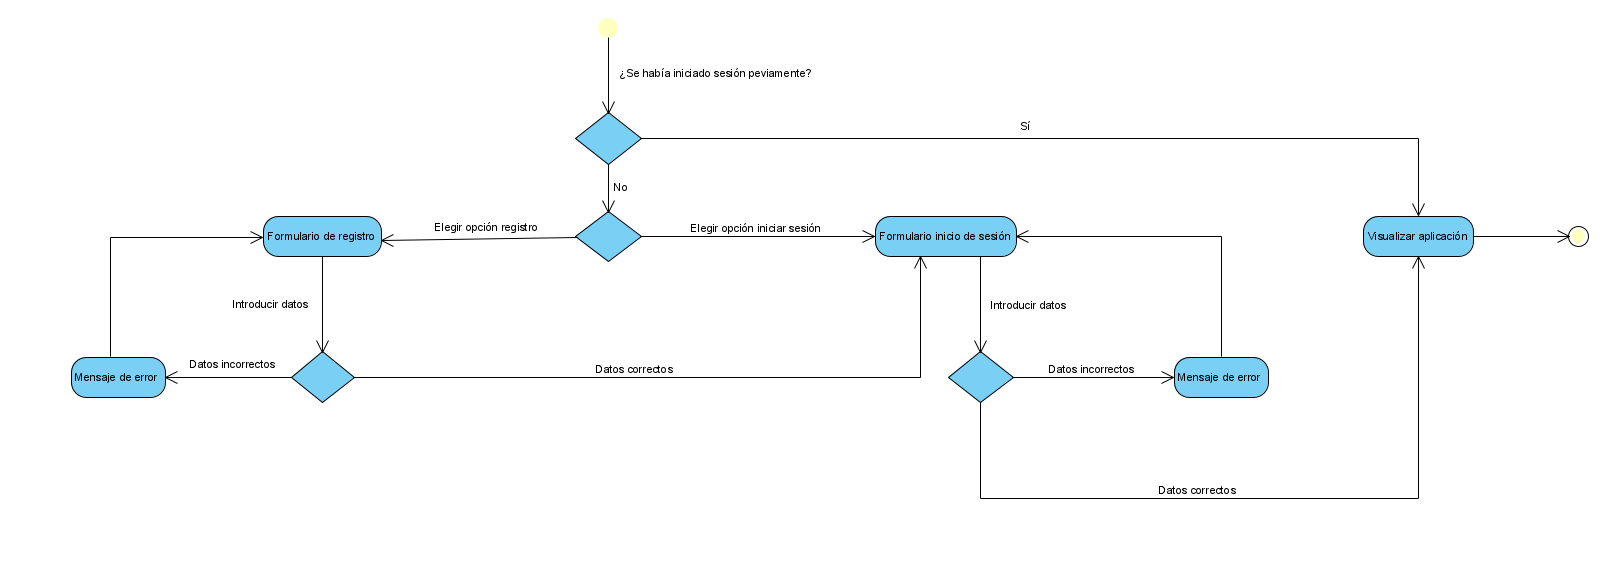
\includegraphics[width=1\textwidth]{figs/diagrama_actividad_usuario_no_registrado.png}
    \caption{Diagrama de actividad de usuario no registrado}
\end{figure}

En este diagrama se observa el proceso que sigue un usuario desde que accede a la aplicación, pasando por las opciones de registro o inicio de sesión, la validación de datos y la visualización de la aplicación, incluyendo el manejo de errores en caso de datos

\begin{figure}[H]
    \centering
    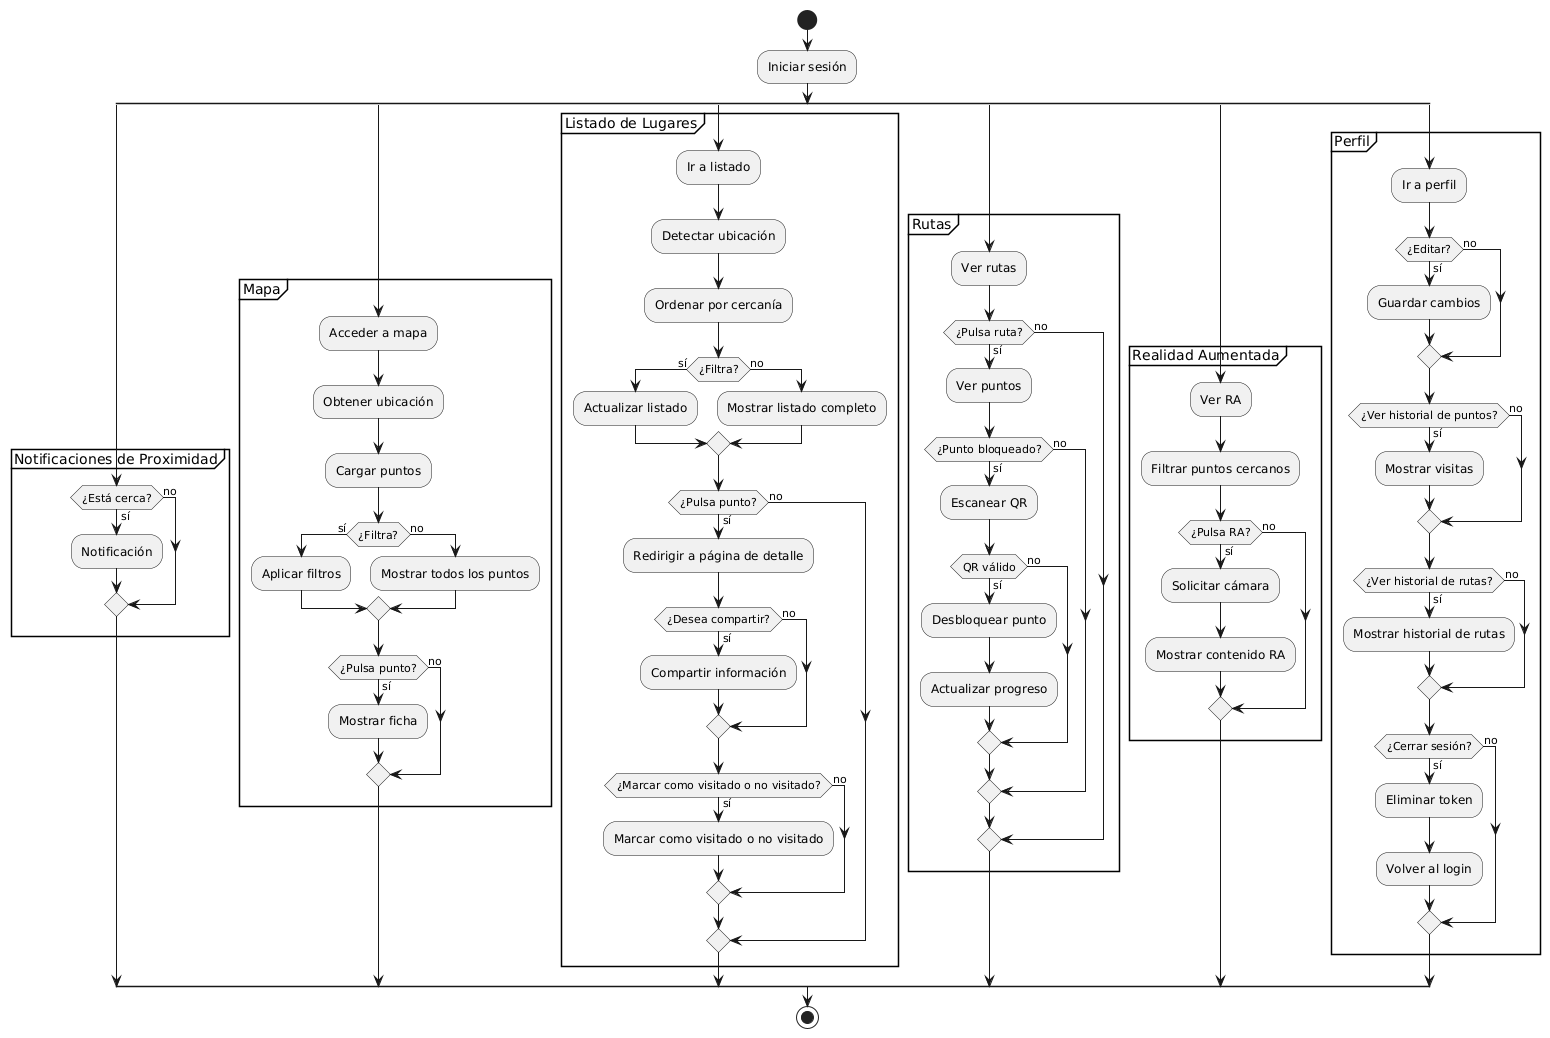
\includegraphics[width=1\textwidth]{figs/diagrama_actividad_usuario_registrado.png}
    \caption{Diagrama de actividad de usuario registrado}
\end{figure}

El diagrama anterior representa el flujo de actividades que puede realizar un usuario registrado, en este caso el administrador, dentro del sistema. Tras iniciar sesión y validar sus credenciales, el administrador accede al panel de administración, donde puede gestionar diferentes entidades del sistema: mujeres históricas, puntos geolocalizados, rutas temáticas, áreas de investigación, materiales multimedia, usuarios y métricas de uso. Cada una de estas gestiones implica la posibilidad de añadir, editar o eliminar información, así como la validación de los datos y la actualización de la base de datos correspondiente. El diagrama muestra cómo estas acciones pueden realizarse de forma paralela e independiente, permitiendo al administrador un control completo sobre los contenidos y usuarios de la aplicación.

\chapter{Diseño}
% !TEX root = ../ejemplo-memoria.tex
% Contenidos del capítulo.
% Las secciones presentadas son orientativas y no representan
% necesariamente la organización que debe tener este capítulo.

% Diagramas de clases, de secuencia, de despliegue, diseño de
% pantallas, etc




\section{Diseño de base de datos}

La base de datos de la aplicación está diseñada para almacenar información sobre mujeres, sus lugares asociados, rutas temáticas, usuarios y el historial de visitas. El diseño sigue una estructura relacional y está implementado en \textbf{PostgreSQL} mediante modelos definidos en Django.

\subsection{Elección de la base de datos y justificación}

Se ha seleccionado \textbf{PostgreSQL} como sistema gestor de base de datos por su robustez, soporte avanzado de tipos de datos, integridad referencial y compatibilidad nativa con Django. PostgreSQL permite almacenar listas de valores en un solo campo, lo que resulta útil para atributos como las áreas de investigación asociadas a cada mujer, sin perder la capacidad de realizar consultas eficientes.

\subsection{Tablas principales y justificación de diseño}

A continuación se describen las tablas principales que conforman el modelo de datos, junto con la justificación de las decisiones tomadas:

\begin{itemize}
    \item \textbf{AreaInvestigacion}: Permite mantener un catálogo normalizado de áreas de investigación, facilitando la gestión y evitando duplicidades.
    \begin{itemize}
        \item \textbf{id} (clave primaria)
        \item \textbf{nombre}: nombre único del área.
    \end{itemize}
    \item \textbf{Mujer}: Representa a una mujer relevante. El campo \texttt{areas\_investigacion} se implementa como un \texttt{ArrayField} de cadenas, aprovechando las capacidades de PostgreSQL para almacenar múltiples áreas directamente en el registro, simplificando la consulta y el filtrado desde la API.
    \begin{itemize}
        \item \textbf{id} (clave primaria)
        \item \textbf{nombre}
        \item \textbf{descripcion}
        \item \textbf{foto}
        \item \textbf{areas\_investigacion}: lista de cadenas de texto (\texttt{ArrayField}) con los nombres de las áreas de investigación asociadas.
        \item \textbf{fechas}: información de fechas relevantes.
    \end{itemize}
    \item \textbf{Lugar}: Almacena información geolocalizada y la relación con una mujer. Se justifica la relación uno-a-muchos para poder asociar varios lugares a una misma mujer.
    \begin{itemize}
        \item \textbf{id} (clave primaria)
        \item \textbf{nombre}
        \item \textbf{descripcion}
        \item \textbf{latitud}
        \item \textbf{longitud}
        \item \textbf{foto}
        \item \textbf{ar\_url}: enlace a contenido de realidad aumentada.
        \item \textbf{mujer\_id} (clave foránea): referencia a la mujer destacada.
    \end{itemize}
    \item \textbf{Ruta}: Agrupa lugares y mujeres en recorridos temáticos. Se emplean relaciones ManyToMany para maximizar la flexibilidad y permitir que una ruta incluya múltiples mujeres y lugares, y viceversa.
    \begin{itemize}
        \item \textbf{id} (clave primaria)
        \item \textbf{nombre}
        \item \textbf{descripcion}
        \item Relación de tipo ManyToMany con las tablas \textbf{Mujer} y \textbf{Lugar}.
    \end{itemize}
    \item \textbf{UserProfile}: Extiende el modelo de usuario de Django para almacenar información adicional relevante para la aplicación, como la fecha de nacimiento.
    \begin{itemize}
        \item \textbf{id} (clave primaria)
        \item \textbf{user\_id} (relación uno a uno con User)
        \item \textbf{birth\_date}
        \item \textbf{email}
    \end{itemize}
    \item \textbf{VisitedLugar}: Permite registrar el historial de visitas de los usuarios a lugares concretos, facilitando la personalización y la obtención de estadísticas.
    \begin{itemize}
        \item \textbf{id} (clave primaria)
        \item \textbf{user\_id} (clave foránea)
        \item \textbf{lugar\_id} (clave foránea)
        \item \textbf{visited\_at}: fecha y hora de la visita.
    \end{itemize}
    \item \textbf{VisitedLugarRuta}: Permite registrar visitas de usuarios a lugares dentro de rutas específicas, lo que posibilita analizar el recorrido de los usuarios y mejorar la experiencia de gamificación.
    \begin{itemize}
        \item \textbf{id} (clave primaria)
        \item \textbf{user\_id} (clave foránea)
        \item \textbf{ruta\_id} (clave foránea)
        \item \textbf{lugar\_id} (clave foránea)
        \item \textbf{visited\_at}: fecha y hora de la visita.
    \end{itemize}
\end{itemize}

\subsection{Relaciones entre tablas}

\begin{itemize}
    \item Un \textbf{Lugar} pertenece a una \textbf{Mujer} (relación uno a muchos).
    \item Una \textbf{Mujer} puede tener varios \textbf{Lugares} asociados.
    \item Una \textbf{Ruta} puede incluir varias \textbf{Mujeres} y varios \textbf{Lugares} (relaciones ManyToMany).
    \item Un \textbf{UserProfile} extiende a un \textbf{User} de Django (relación uno a uno).
    \item \textbf{VisitedLugar} y \textbf{VisitedLugarRuta} permiten registrar el historial de visitas de los usuarios, tanto de lugares individuales como de lugares dentro de rutas.
\end{itemize}

\subsection{Esquema de tablas}

El siguiente esquema resume la estructura de las tablas principales de la base de datos. Para mejorar la visualización y evitar cortes de línea, se utiliza el entorno \texttt{tabularx}:

\begin{table}[H]
\centering
\begin{tabularx}{\textwidth}{l X}
\textbf{Tabla} & \textbf{Campos principales} \\
\hline
Mujer & id, nombre, descripcion, foto, areas\_investigacion (ArrayField), fechas \\
Lugar & id, nombre, descripcion, latitud, longitud, foto, ar\_url, mujer\_id (FK) \\
Ruta & id, nombre, descripcion, mujeres (M2M), lugares (M2M) \\
UserProfile & id, user\_id (O2O), birth\_date, email \\
VisitedLugar & id, user\_id (FK), lugar\_id (FK), visited\_at \\
VisitedLugarRuta & id, user\_id (FK), ruta\_id (FK), lugar\_id (FK), visited\_at \\
AreaInvestigacion & id, nombre \\
\end{tabularx}
\caption{Esquema resumido de las tablas principales de la base de datos}
\end{table}

\subsection{Justificación global del diseño}

El modelo de datos relacional implementado garantiza la integridad y la eficiencia en las consultas. El uso de \texttt{ArrayField} en \textbf{Mujer} permite una mayor flexibilidad y rendimiento en la consulta de áreas de investigación, sin necesidad de realizar joins adicionales, lo que es especialmente útil para filtros rápidos en la API. Las tablas de historial de visitas están separadas para facilitar la obtención de estadísticas, la personalización de la experiencia del usuario y la escalabilidad futura (por ejemplo, para añadir logros o recomendaciones personalizadas).
\begin{landscape}
    \begin{figure}
        \centering
        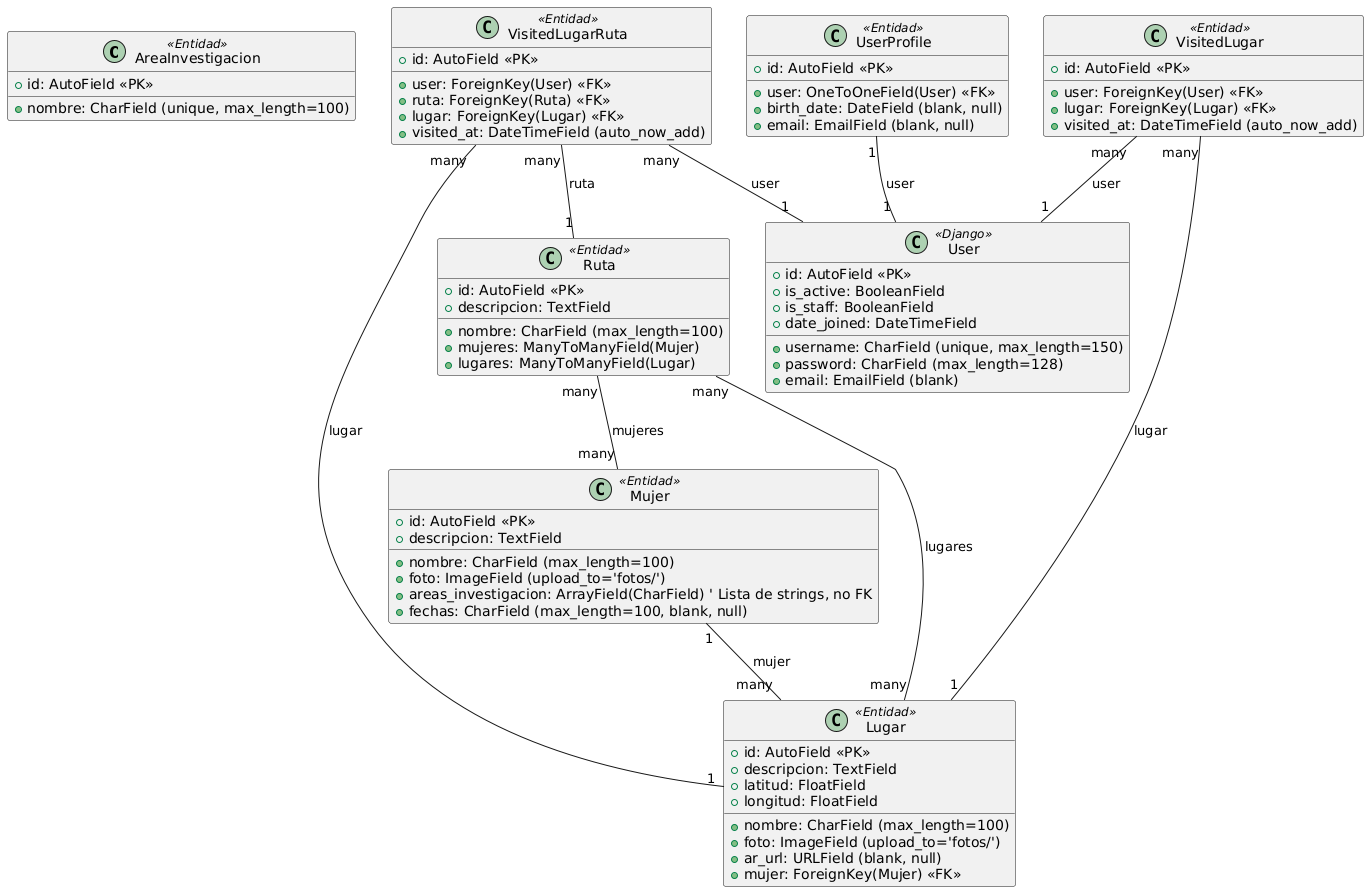
\includegraphics[width=1.2\paperwidth]{figs/diagrama_clases.png}
        \caption{Diagrama de clases de la base de datos}
    \end{figure}
\end{landscape}
\section{Diseño de la arquitectura del frontend}

El frontend de la aplicación está desarrollado en \textbf{React Native}, siguiendo una arquitectura basada en componentes funcionales y el uso de contextos para la gestión eficiente del estado global.El hecho de que el diseño sea modular y esté desacoplado hace que sea más sencillo de mantener y escalar, además de permitir añadir nuevas funcionalidades sin complicaciones. Esto también ayuda a que la experiencia de usuario sea más fácil de adaptar en un futuro con nuevas necesidades.

\subsection{Diagrama de clases del frontend}

La Figura~\ref{fig:clases-frontend} muestra el diagrama de clases que representa la arquitectura principal del frontend. Los componentes se agrupan en paquetes según su responsabilidad funcional: contextos, navegación, usuario, rutas, lugares y utilidades.

\begin{itemize} \item \textbf{Contextos:} El componente \texttt{FiltrosContext} centraliza la gestión del estado global de los filtros aplicados en la aplicación, proporcionando métodos para su actualización y reseteo. Este contexto es consumido por componentes como \texttt{Filtros}, \texttt{Rutas} y \texttt{Mapa}, permitiendo la sincronización de los criterios de filtrado en toda la interfaz. \item \textbf{Navegación:} El componente \texttt{NavigationApp} implementa la navegación principal mediante un \textit{stack navigator}, gestionando el flujo entre pantallas y facilitando la transición entre las distintas funcionalidades de la app. \item \textbf{Componentes de Usuario:} Incluyen las pantallas de autenticación (\texttt{Login}, \texttt{Register}), el perfil de usuario (\texttt{PerfilUsuario}) y el acceso al historial de lugares y rutas visitadas (\texttt{HistorialLugares}, \texttt{HistorialRutas}). Cada uno de estos componentes gestiona su propio estado y lógica de interacción, garantizando la personalización y seguridad de la experiencia de usuario. \item \textbf{Componentes de Rutas y Lugares:} \texttt{Rutas} y \texttt{Mapa} permiten al usuario explorar rutas temáticas y lugares geolocalizados, respectivamente. Los componentes \texttt{Detail}, \texttt{HistorialLugares} y \texttt{HistorialRutas} permiten consultar información detallada de los lugares y el registro de visitas de estos, integrando la lógica de interacción con el backend. \item \textbf{Componentes de Utilidad:} Incluyen \texttt{Filtros}, \texttt{Mujeres} (visualización combinada de mujeres y lugares), la pantalla de bienvenida (\texttt{Welcome}), la lógica de realidad aumentada (\texttt{AR}), y la lógica de notificaciones de proximidad (\texttt{NotificacionProximidad}), que se ejecuta de forma invisible para el usuario y activa notificaciones según la localización. \end{itemize}

Las relaciones entre componentes reflejan tanto el consumo de contexto (\textit{consume}), como la navegación entre pantallas (\textit{navega a}), y el uso de lógica auxiliar (por ejemplo, la integración de notificaciones en el componente principal \texttt{Main}).

\begin{landscape} \vfill \begin{figure}[H] \centering 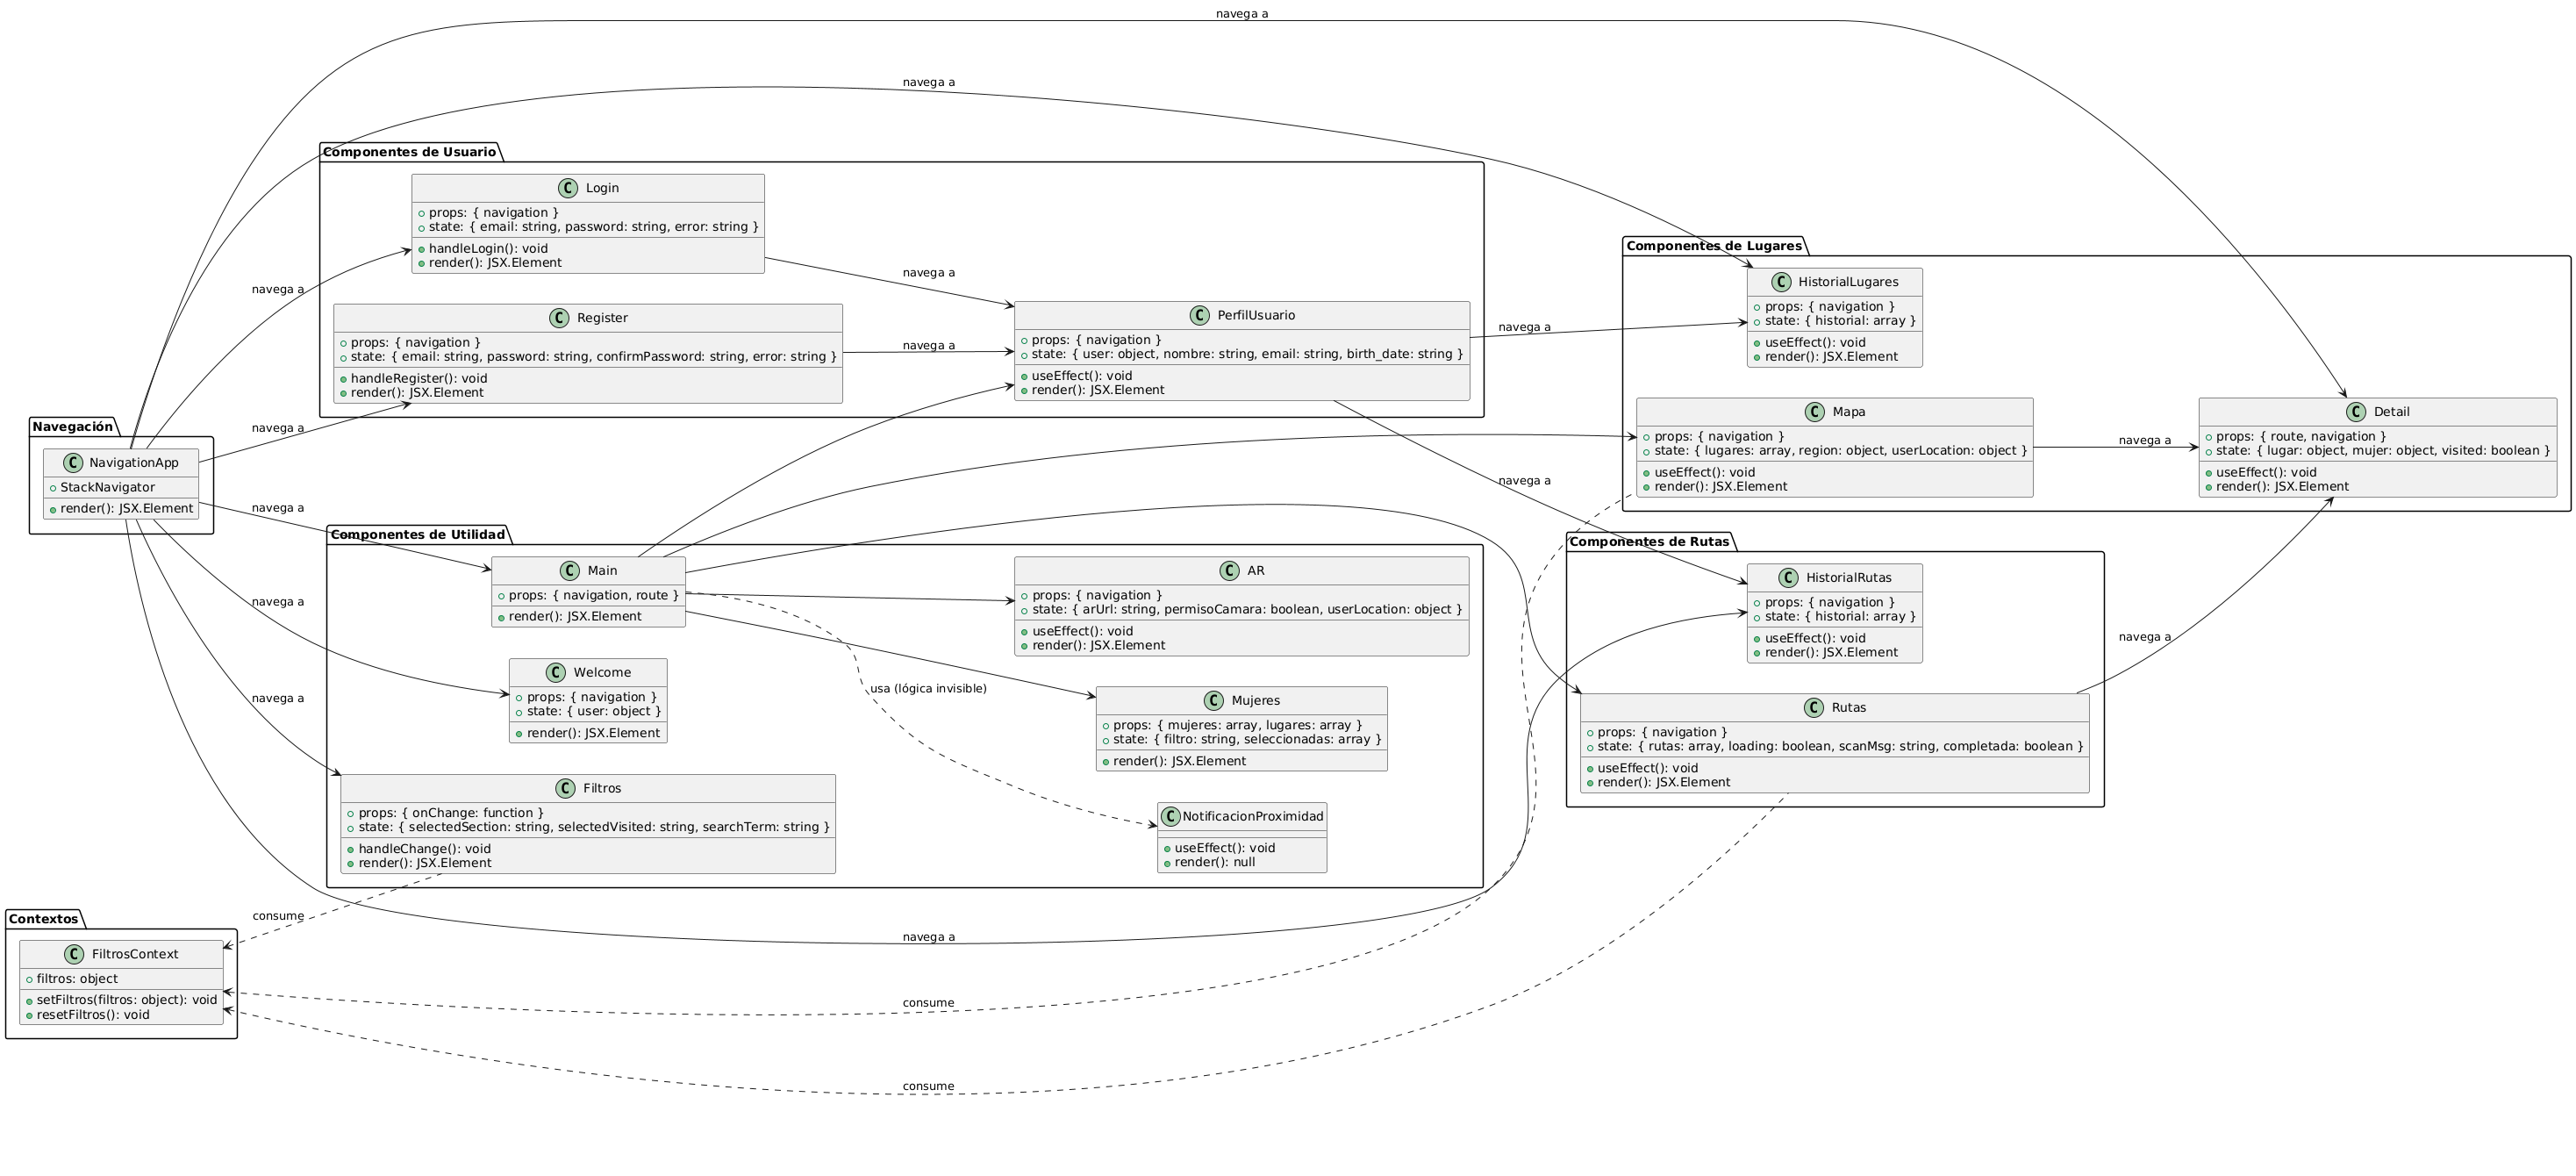
\includegraphics[width=1.2\paperwidth]{figs/prueba.png} \caption{Diagrama de clases del frontend React Native: estructura de componentes y relaciones principales.} \label{fig:clases-frontend} \end{figure} \vfill \end{landscape}

\section{Diagramas de secuencia}

Los diagramas de secuencia muestran cómo interactúan los distintos elementos del sistema a lo largo del tiempo para llevar a cabo un caso de uso concreto. Representan visualmente el flujo de mensajes entre actores (como el usuario o el administrador) y los componentes internos del sistema (como la aplicación, la base de datos o servicios de autenticación). 

En esta sección se presentan los diagramas de secuencia correspondientes a cada uno de los casos de uso definidos en el análisis de requisitos del sistema, descritos en el apartado~\ref{sec:casos-uso} (Especificación de casos de uso). 


\subsection{Diagrama de secuencia del caso de uso 1: Login de usuario}
\begin{figure}[H]
    \centering
    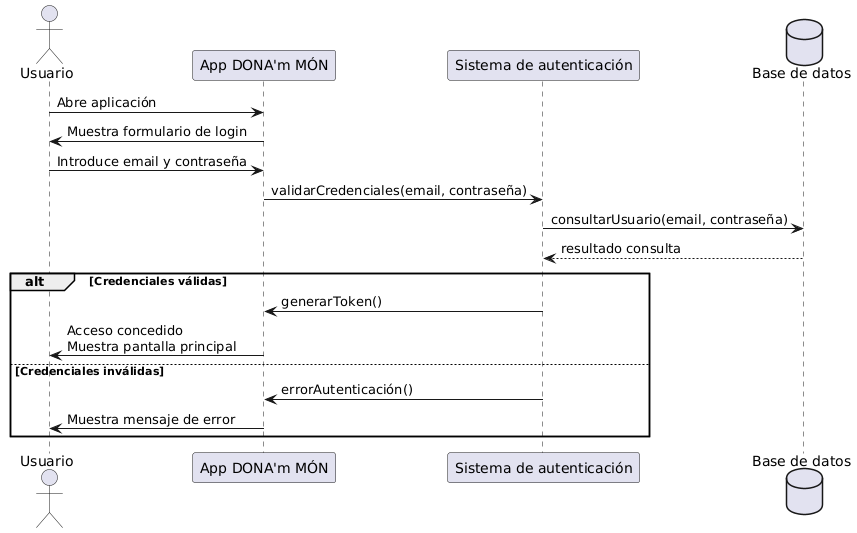
\includegraphics[width=0.8\textwidth]{figs/caso1.png}
    \caption{Diagrama de secuencia del caso de uso 1: Login de usuario}
\end{figure}

\clearpage
\subsection{Diagrama de secuencia del caso de uso 2: Registro de usuario}
\begin{figure}[H]
    \centering
    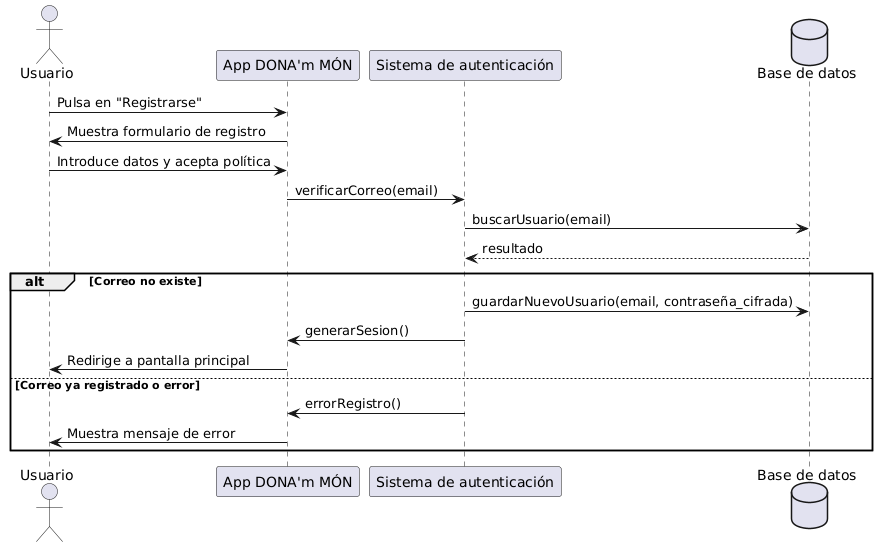
\includegraphics[width=0.8\textwidth]{figs/caso2.png}
    \caption{Diagrama de secuencia del caso de uso 2: Registro de usuario}
\end{figure}

\subsection{Diagrama de secuencia del caso de uso 3: Ver mapa con puntos de interés}
\begin{figure}[H]
    \centering
    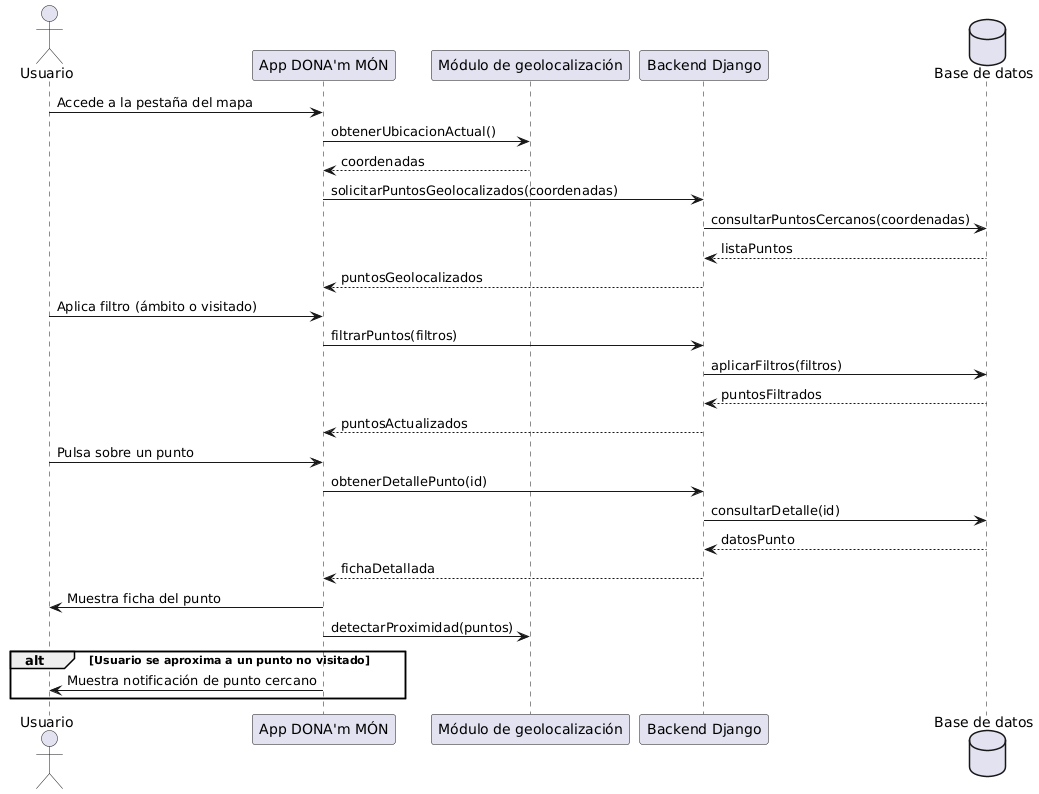
\includegraphics[width=0.8\textwidth]{figs/caso3.png}
    \caption{Diagrama de secuencia del caso de uso 3: Ver mapa con puntos de interés}
\end{figure}

\subsection{Diagrama de secuencia del caso de uso 4: Ver listado de puntos ordenado por cercanía}
\begin{figure}[H]
    \centering
    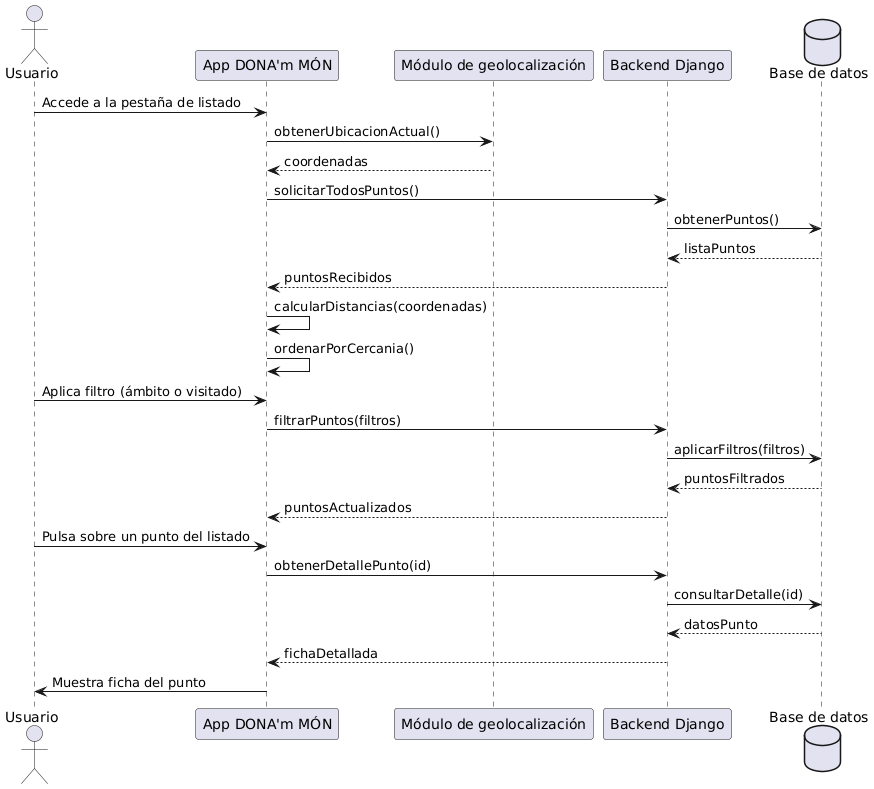
\includegraphics[width=0.8\textwidth]{figs/caso4.png}
    \caption{Diagrama de secuencia del caso de uso 4: Ver listado de puntos ordenado por cercanía}
\end{figure}

\subsection{Diagrama de secuencia del caso de uso 5: Ver ficha del lugar}
\begin{figure}[H]
    \centering
    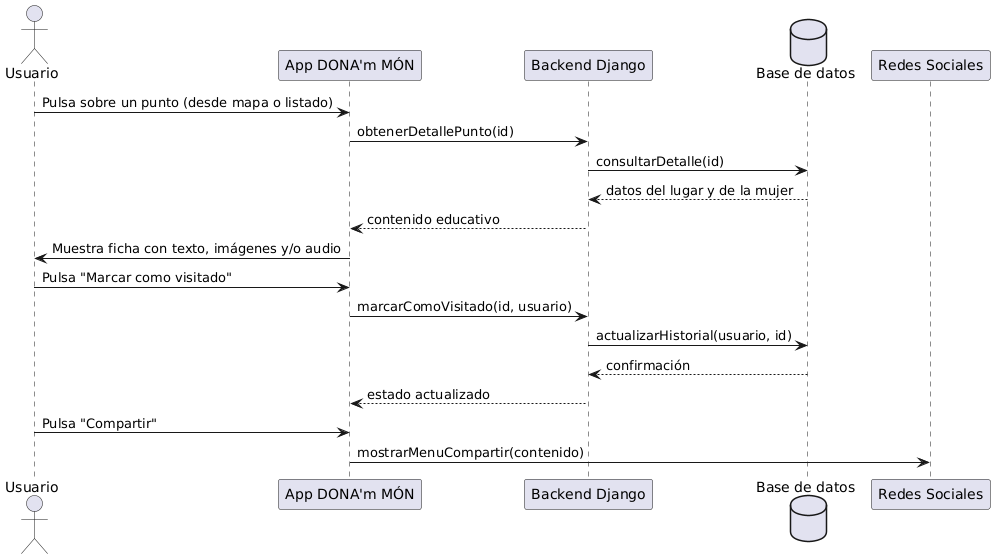
\includegraphics[width=0.8\textwidth]{figs/caso5.png}
    \caption{Diagrama de secuencia del caso de uso 5: Ver ficha del lugar}
\end{figure}

\subsection{Diagrama de secuencia del caso de uso 6: Ver rutas y consultar puntos de una ruta}
\begin{figure}[H]
    \centering
    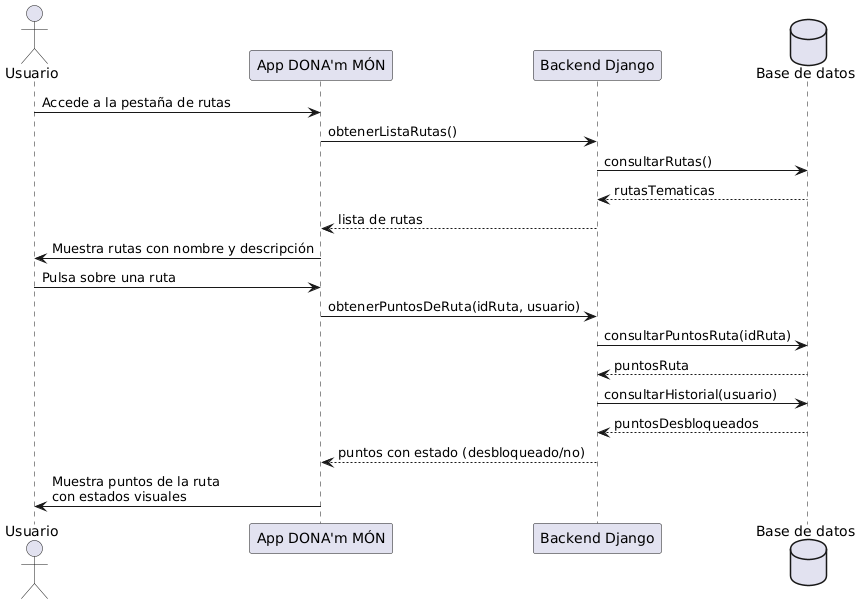
\includegraphics[width=0.8\textwidth]{figs/caso6.png}
    \caption{Diagrama de secuencia del caso de uso 6: Ver rutas y consultar puntos de una ruta}
\end{figure}

\subsection{Diagrama de secuencia del caso de uso 7: Escanear QR de punto de ruta}
\begin{figure}[H]
    \centering
    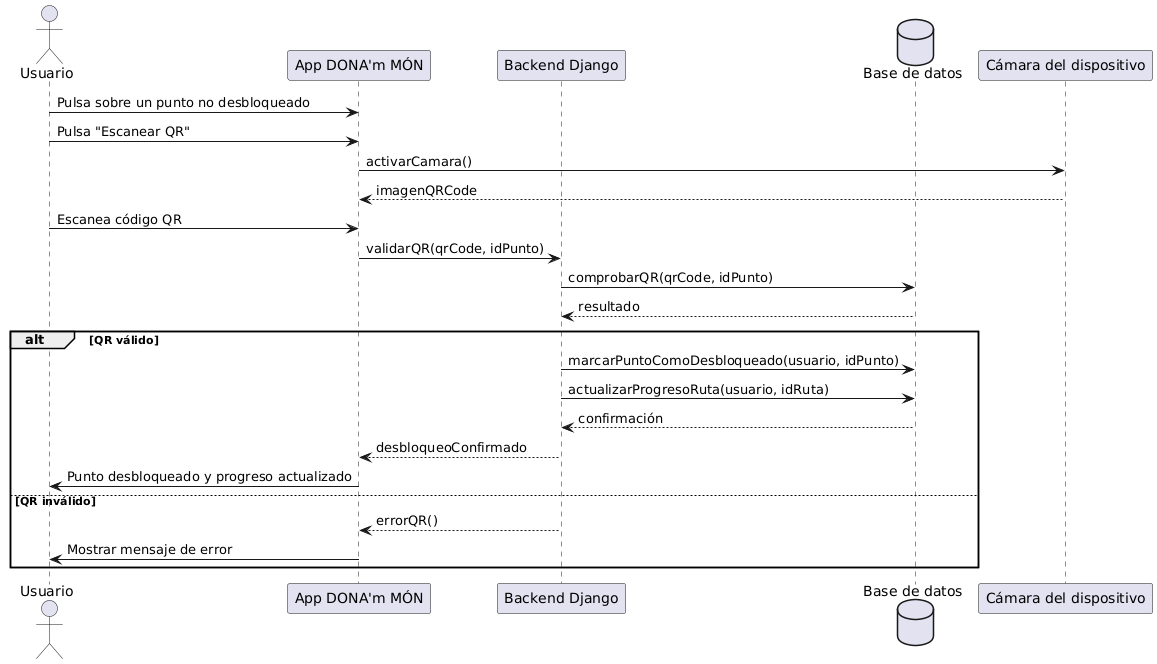
\includegraphics[width=0.8\textwidth]{figs/caso7.png}
    \caption{Diagrama de secuencia del caso de uso 7: Escanear QR de punto de ruta}
\end{figure}

\subsection{Diagrama de secuencia del caso de uso 8: Ver puntos RA disponibles}
\begin{figure}[H]
    \centering
    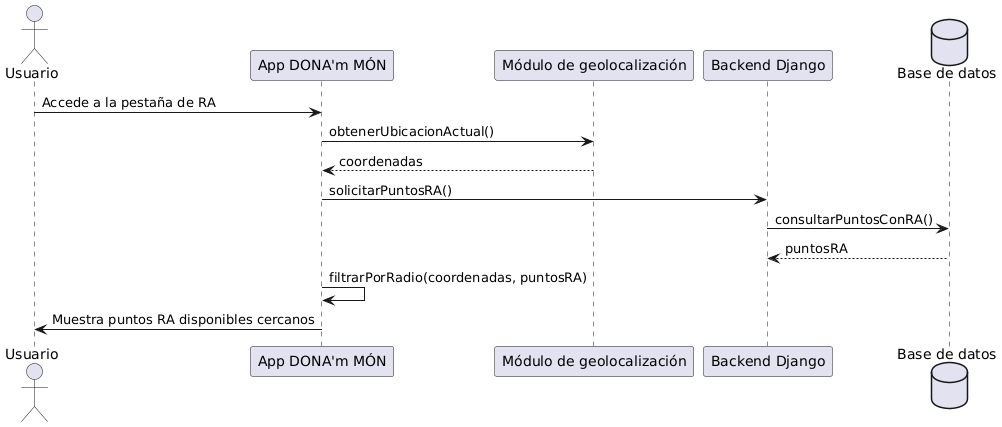
\includegraphics[width=0.8\textwidth]{figs/caso8.png}
    \caption{Diagrama de secuencia del caso de uso 8: Ver puntos RA disponibles}
\end{figure}

\subsection{Diagrama de secuencia del caso de uso 9: Visualizar contenido RA}
\begin{figure}[H]
    \centering
    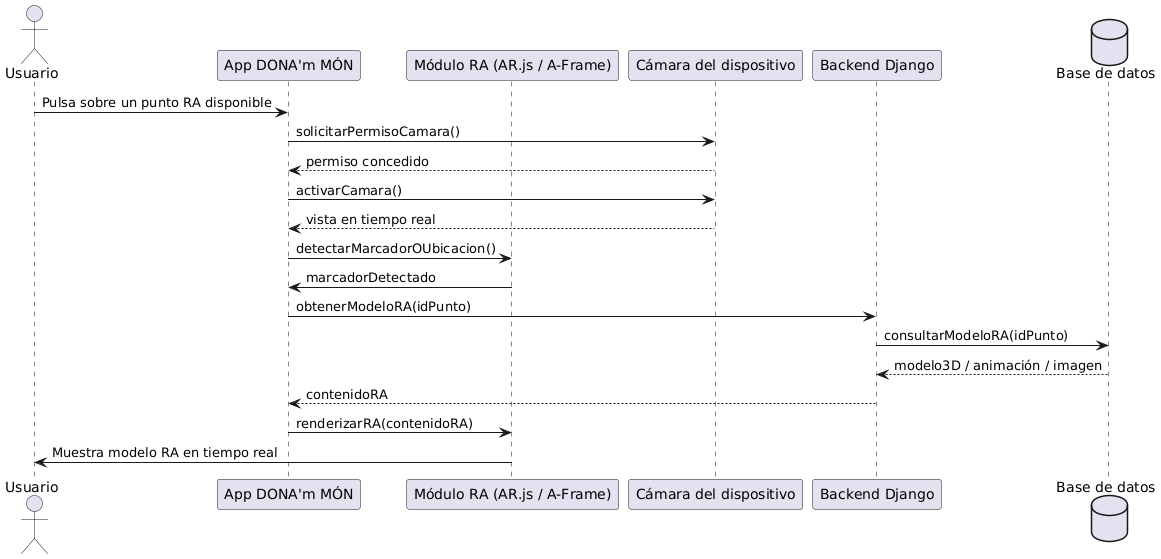
\includegraphics[width=0.8\textwidth]{figs/caso9.png}
    \caption{Diagrama de secuencia del caso de uso 9: Visualizar contenido RA}
\end{figure}

\subsection{Diagrama de secuencia del caso de uso 10: Editar perfil de usuario}
\begin{figure}[H]
    \centering
    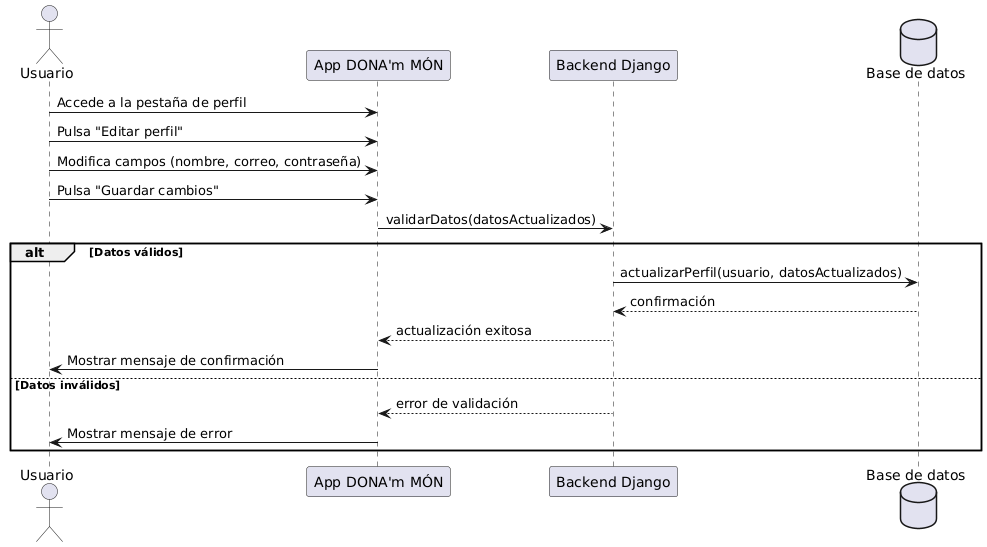
\includegraphics[width=0.8\textwidth]{figs/caso10.png}
    \caption{Diagrama de secuencia del caso de uso 10: Editar perfil de usuario}
\end{figure}

\subsection{Diagrama de secuencia del caso de uso 11: Ver historial de lugares visitados y rutas completadas}
\begin{figure}[H]
    \centering
    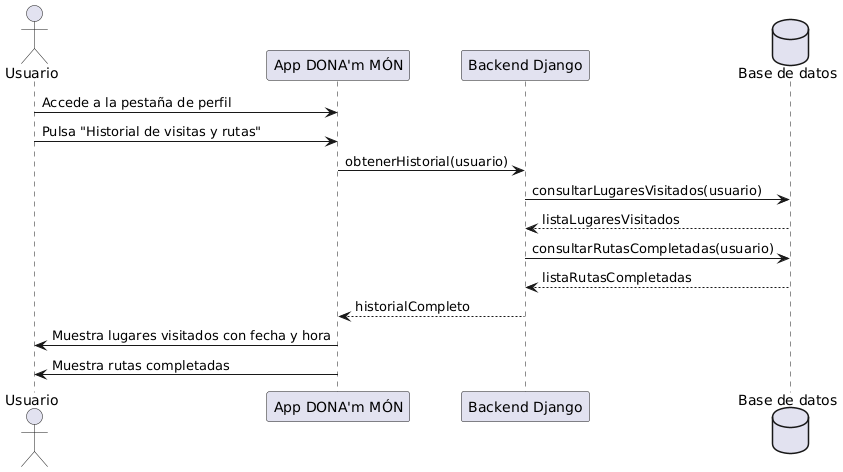
\includegraphics[width=0.8\textwidth]{figs/caso11.png}
    \caption{Diagrama de secuencia del caso de uso 11: Ver historial de lugares visitados y rutas completadas}
\end{figure}

\subsection{Diagrama de secuencia del caso de uso 12: Cerrar sesión}
\begin{figure}[H]
    \centering
    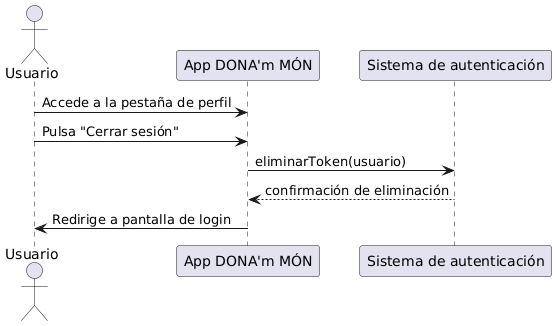
\includegraphics[width=0.8\textwidth]{figs/caso12.png}
    \caption{Diagrama de secuencia del caso de uso 12: Cerrar sesión}
\end{figure}

\subsection{Diagrama de secuencia del caso de uso 13: Iniciar sesión como administrador}
\begin{figure}[H]
    \centering
    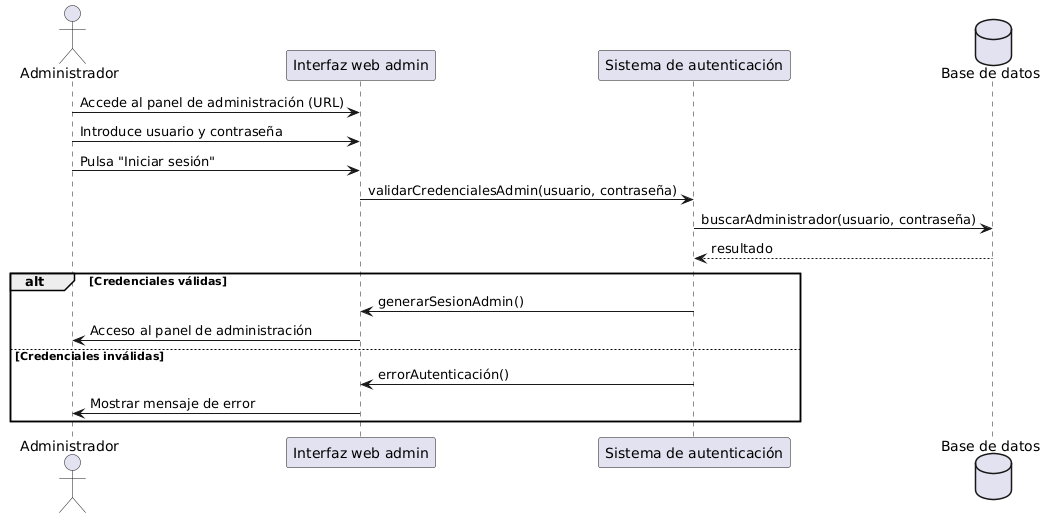
\includegraphics[width=0.8\textwidth]{figs/caso13.png}
    \caption{Diagrama de secuencia del caso de uso 13: Iniciar sesión como administrador}
\end{figure}

\subsection{Diagrama de secuencia del caso de uso 14: Gestionar mujeres históricas}
\begin{figure}[H]
    \centering
    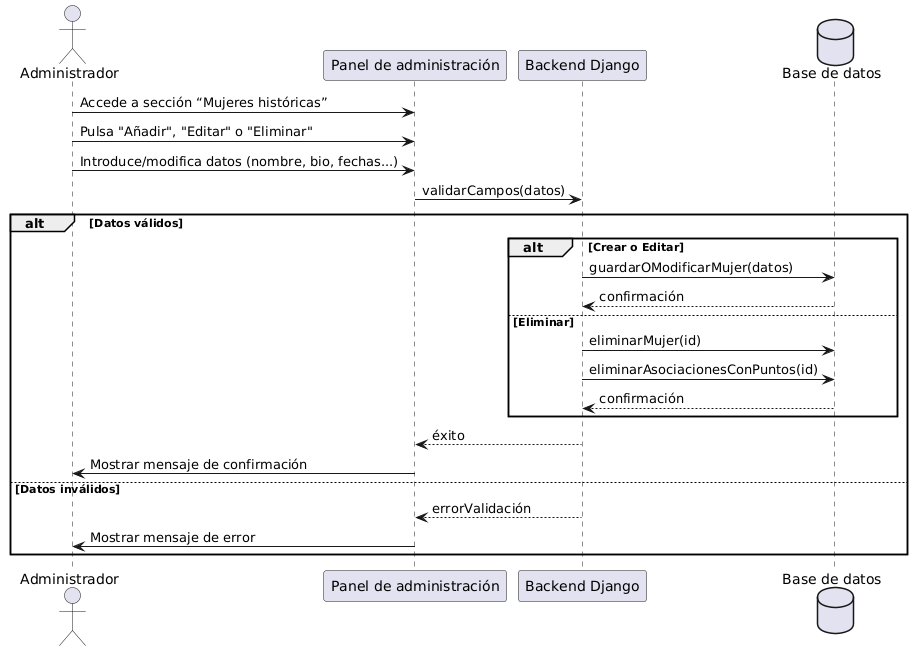
\includegraphics[width=0.8\textwidth]{figs/caso14.png}
    \caption{Diagrama de secuencia del caso de uso 14: Gestionar mujeres históricas}
\end{figure}

\subsection{Diagrama de secuencia del caso de uso 15: Gestionar puntos geolocalizados}
\begin{figure}[H]
    \centering
    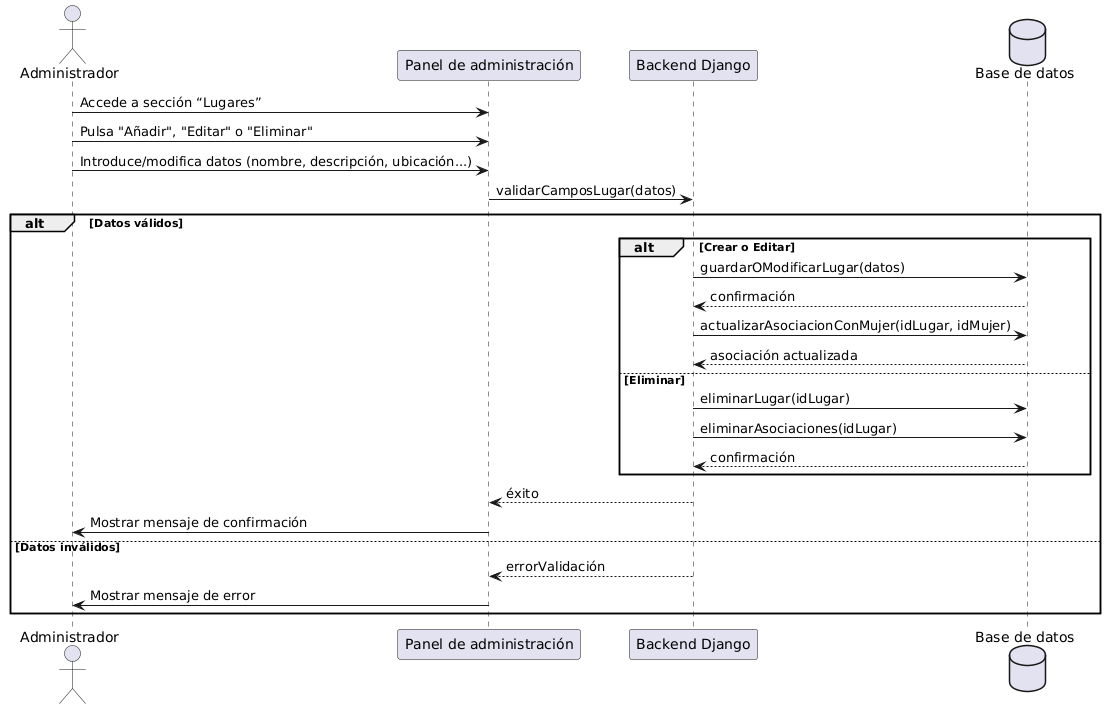
\includegraphics[width=0.8\textwidth]{figs/caso15.png}
    \caption{Diagrama de secuencia del caso de uso 15: Gestionar puntos geolocalizados}
\end{figure}

\subsection{Diagrama de secuencia del caso de uso 16: Gestionar rutas temáticas}
\begin{figure}[H]
    \centering
    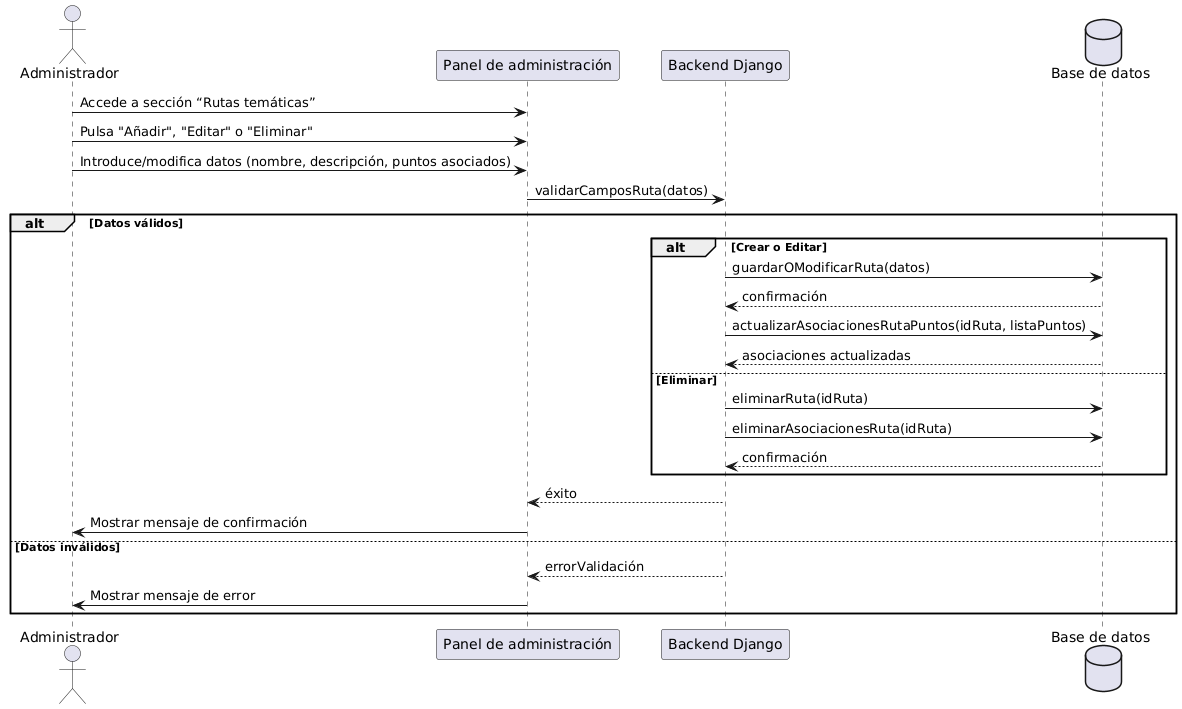
\includegraphics[width=0.8\textwidth]{figs/caso16.png}
    \caption{Diagrama de secuencia del caso de uso 16: Gestionar rutas temáticas}
\end{figure}

\subsection{Diagrama de secuencia del caso de uso 17: Consultar lista de usuarios}
\begin{figure}[H]
    \centering
    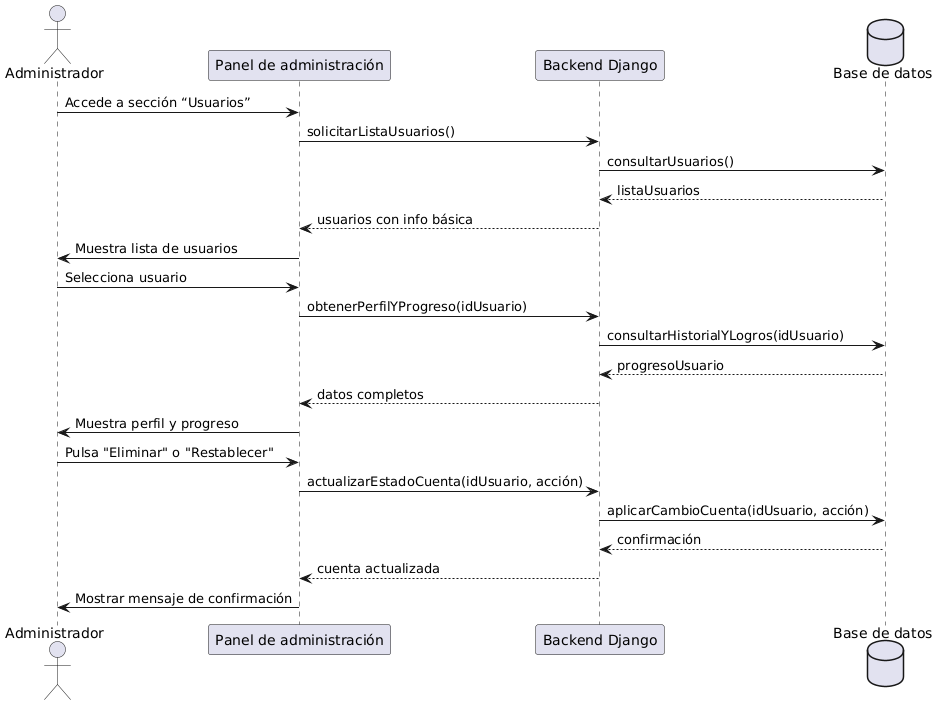
\includegraphics[width=0.8\textwidth]{figs/caso17.png}
    \caption{Diagrama de secuencia del caso de uso 17: Consultar lista de usuarios}
\end{figure}

\subsection{Diagrama de secuencia del caso de uso 18: Gestionar materiales multimedia}
\begin{figure}[H]
    \centering
    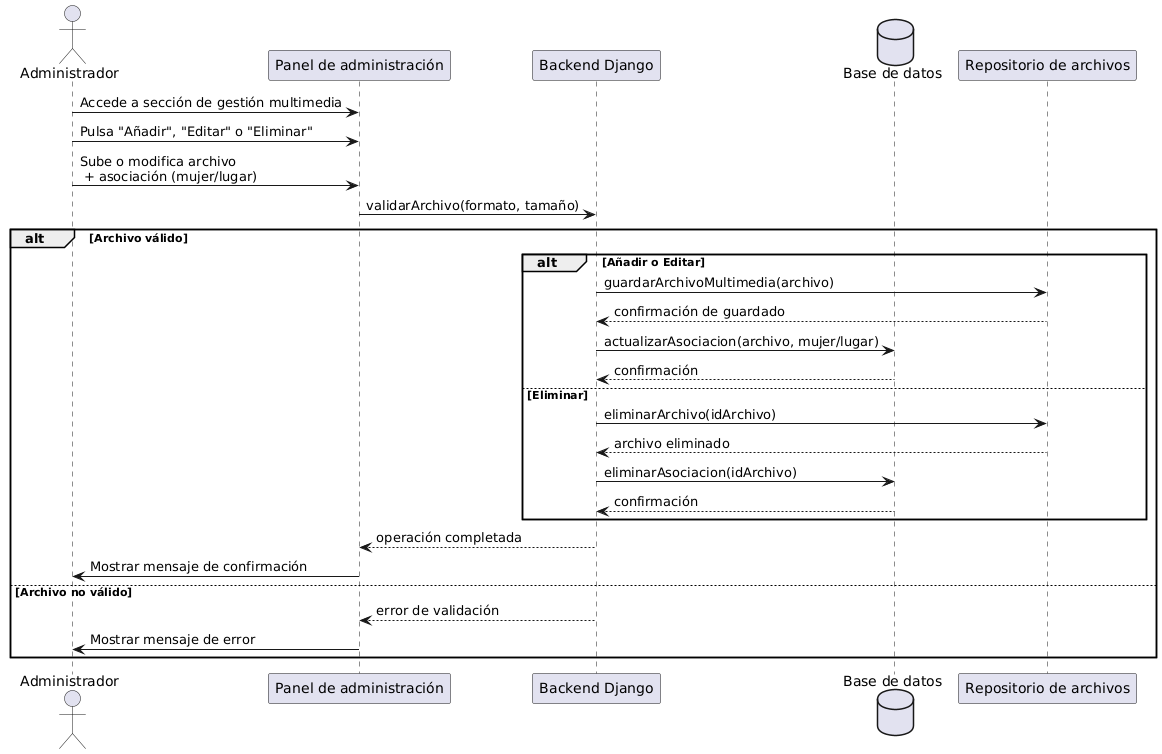
\includegraphics[width=0.8\textwidth]{figs/caso18.png}
    \caption{Diagrama de secuencia del caso de uso 18: Gestionar materiales multimedia}
\end{figure}

\subsection{Diagrama de secuencia del caso de uso 19: Consultar métricas de uso}
\begin{figure}[H]
    \centering
    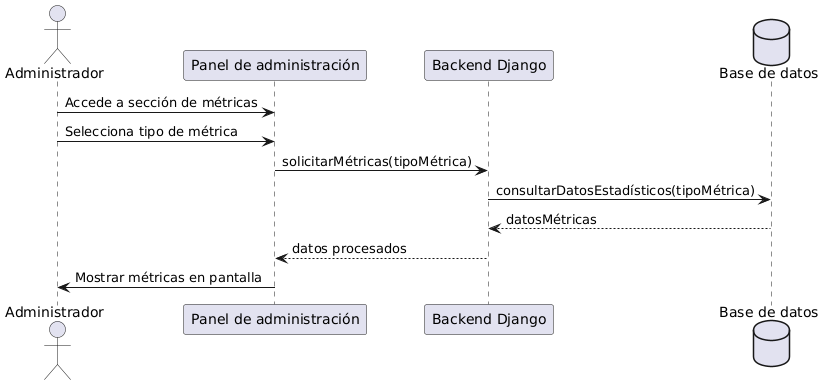
\includegraphics[width=0.8\textwidth]{figs/caso19.png}
    \caption{Diagrama de secuencia del caso de uso 19: Consultar métricas de uso}
\end{figure}

\subsection{Diagrama de secuencia del caso de uso 20: Gestionar áreas de investigación}
\begin{figure}[H]
    \centering
    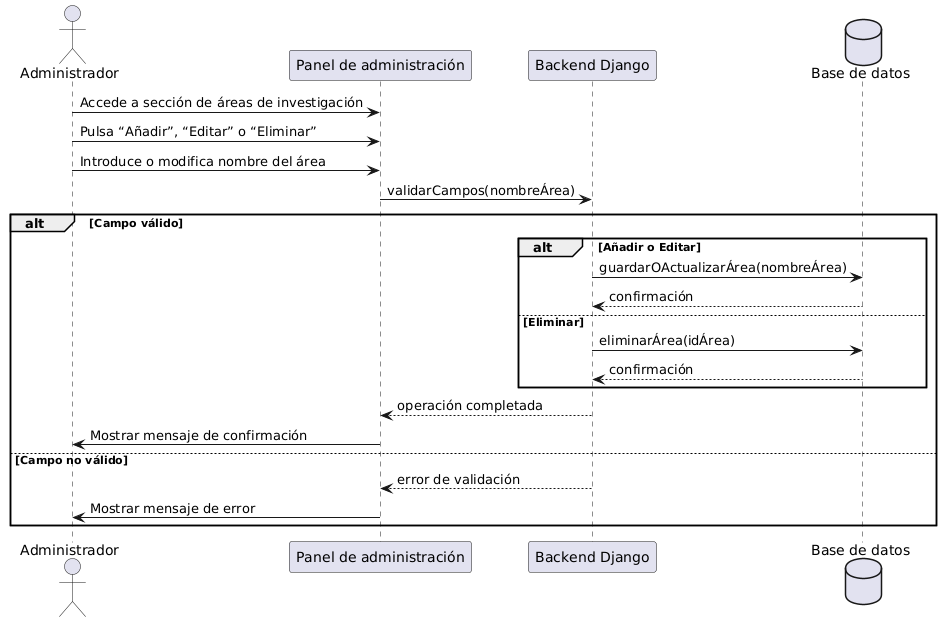
\includegraphics[width=0.8\textwidth]{figs/caso20.png}
    \caption{Diagrama de secuencia del caso de uso 20: Gestionar áreas de investigación}
\end{figure}

\chapter{Implementación y pruebas}
% !TEX root = ../ejemplo-memoria.tex
\section{Implementación del backend}

\subsection{Herramientas, frameworks y lenguajes utilizados}

El backend de la aplicación se ha desarrollado utilizando el framework \textbf{Django} (versión 5.2.2) junto con \textbf{Django REST Framework} para la construcción de la API. Django facilita la definición de modelos, la gestión de usuarios y la exposición de endpoints RESTful de manera segura y eficiente.

Para la persistencia de datos se ha empleado \textbf{PostgreSQL} como sistema gestor de bases de datos relacional. El entorno de desarrollo y despliegue se ha gestionado mediante \textbf{Docker} y \textbf{Docker Compose}, lo que permite la portabilidad y la replicabilidad del entorno en diferentes máquinas.

Las principales herramientas y librerías utilizadas son:
\begin{itemize}
    \item \textbf{Python 3.10}
    \item \textbf{Django 5.2.2} 
    \item \textbf{Django REST Framework} (\texttt{djangorestframework})
    \item \textbf{Docker} y \textbf{Docker Compose} para la gestión de contenedores
    \item \texttt{psycopg2-binary} para la conexión con PostgreSQL
    \item \texttt{django-cors-headers} para permitir peticiones desde el frontend
    \item \texttt{Pillow} para el manejo de imágenes en Django
\end{itemize}
\subsection{Estructura del proyecto y organización del código}

El código fuente del backend se encuentra en la carpeta \texttt{donam-mon-backend/}, que contiene la configuración de Docker, los archivos de requisitos y el proyecto Django propiamente dicho. La estructura principal es la siguiente:

\begin{lstlisting}[language=bash, caption={Estructura principal del backend}]
donam-mon-backend/
    docker-compose.yml
    Dockerfile
    requirements.txt

    backend/
        manage.py
        db.sqlite3

        config/
            __init__.py
            asgi.py
            settings.py
            urls.py
            wsgi.py

        mujeres/
            __init__.py
            admin.py
            apps.py
            models.py
            serializers.py
            tests.py
            views.py

            migrations/
\end{lstlisting}

\texttt{config/}: Contiene la configuración global del proyecto Django (ajustes, rutas principales, etc.).

\texttt{mujeres/}: Es la aplicación principal, donde se definen los modelos, vistas, serializers, administración y lógica de negocio.

\subsection{Modelado de datos}

El modelado de datos es uno de los aspectos más relevantes del backend. Se han definido modelos para representar mujeres relevantes, lugares asociados, rutas temáticas, usuarios y el historial de visitas. A continuación se muestra un fragmento representativo del modelo \texttt{Mujer}:

\begin{lstlisting}[language=Python, caption={Modelo Mujer}, escapeinside={(*@}{@*)}]
class Mujer(models.Model):
    nombre = models.CharField(max_length=100)
    descripcion = models.TextField()
    foto = models.ImageField(upload_to='fotos/', blank=True, null=True)
    areas_investigacion = ArrayField(
        models.CharField(max_length=100), blank=True, default=list, verbose_name='Áreas de investigación'
    )
    fechas = models.CharField(max_length=100, blank=True, null=True)
\end{lstlisting}

\
Se ha optado por utilizar \texttt{ArrayField} para el campo \texttt{areas\_investigacion} en el modelo \texttt{Mujer}, aprovechando la capacidad de PostgreSQL para almacenar listas de cadenas en un solo campo. Esta decisión permite simplificar el modelo, evitar tablas intermedias y realizar búsquedas y filtrados eficientes desde la API, facilitando la integración con el frontend. Se evaluó el uso de \texttt{ManyToManyField}, pero se descartó por la simplicidad y rendimiento que ofrece \texttt{ArrayField} en este caso.

El modelo \texttt{Lugar} representa los lugares geolocalizados asociados a una mujer, e incluye campos para la latitud, longitud, foto y un enlace a contenido de realidad aumentada.
En lugar de almacenar los modelos 3D directamente en la base de datos o en el propio backend, se ha optado por subir los archivos 3D y el HTML necesario a un repositorio externo (GitHub Pages) y guardar únicamente la URL de acceso en el campo \texttt{ar\_url}.
De esta forma, la base de datos y el backend no se ven saturados con archivos grandes ni con peticiones de contenido estático. Además, al utilizar servicios externos optimizados para servir archivos estáticos y contenido web se mejora tanto la velocidad de carga como la escalabilidad de la aplicación. Así, el campo \texttt{ar\_url} actúa como referencia a la experiencia de realidad aumentada, permitiendo que el frontend acceda directamente al recurso externo de forma eficiente y desacoplada del backend. Esta estrategia también facilita la actualización y gestión de los modelos 3D y sus visores HTML, ya que no es necesario modificar ni desplegar el backend cada vez que se realiza un cambio en estos recursos.

\begin{lstlisting}[language=Python, caption={Modelo Lugar}, escapeinside={(*@}{@*)}]
class Lugar(models.Model):
    nombre = models.CharField(max_length=100)
    descripcion = models.TextField()
    latitud = models.FloatField(blank=True, null=True)
    longitud = models.FloatField(blank=True, null=True)
    foto = models.ImageField(upload_to='fotos/', blank=True, null=True)
    ar\_url = models.URLField(max_length=300, blank=True, null=True, verbose_name='URL de Realidad Aumentada')
    mujer = models.ForeignKey(Mujer, on_delete=models.CASCADE, related_name='lugares')
\end{lstlisting}

El modelo \texttt{Ruta} agrupa lugares y mujeres en recorridos temáticos, utilizando relaciones \texttt{ManyToManyField} para maximizar la flexibilidad:

\begin{lstlisting}[language=Python, caption={Modelo Ruta}]
class Ruta(models.Model):
    nombre = models.CharField(max_length=100, unique=True)
    descripcion = models.TextField(blank=True)
    mujeres = models.ManyToManyField(Mujer, related_name='rutas', blank=True)
    lugares = models.ManyToManyField(Lugar, related_name='rutas', blank=True)
\end{lstlisting}

Para la gestión de usuarios se utiliza el modelo estándar de Django, extendido mediante un modelo \texttt{UserProfile} que almacena información adicional relevante para la aplicación:

\begin{lstlisting}[language=Python, caption={Modelo UserProfile}]
class UserProfile(models.Model):
    user = models.OneToOneField(User, on_delete=models.CASCADE, related_name='profile')
    birth_date = models.DateField(blank=True, null=True)
    email = models.EmailField(blank=True, null=True)
\end{lstlisting}

El historial de visitas se gestiona con los modelos \texttt{VisitedLugar} y \texttt{VisitedLugarRuta}, que permiten registrar tanto visitas individuales como visitas dentro de rutas temáticas:

\begin{lstlisting}[language=Python, caption={Modelo VisitedLugar}]
class VisitedLugar(models.Model):
    user = models.ForeignKey(User, on_delete=models.CASCADE, related_name='visited_lugares')
    lugar = models.ForeignKey(Lugar, on_delete=models.CASCADE, related_name='visitas')
    visited_at = models.DateTimeField(auto_now_add=True)
\end{lstlisting}

\begin{lstlisting}[language=Python, caption={Modelo VisitedLugarRuta}]
class VisitedLugarRuta(models.Model):
    user = models.ForeignKey(User, on_delete=models.CASCADE, related_name='visited_lugares_ruta')
    ruta = models.ForeignKey(Ruta, on_delete=models.CASCADE, related_name='visitas')
    lugar = models.ForeignKey(Lugar, on_delete=models.CASCADE, related_name='visitas_ruta')
    visited_at = models.DateTimeField(auto_now_add=True)
\end{lstlisting}

\subsection{Gestión de imágenes}

Para la gestión de imágenes, se utiliza el campo \texttt{ImageField} en los modelos. En la configuración de Django se define la ruta de almacenamiento y la URL de acceso a los archivos subidos:

\begin{lstlisting}[language=Python, caption={Configuración de imágenes en settings.py}]
MEDIA_URL = '/fotos/'
MEDIA_ROOT = os.path.join(BASE_DIR, 'fotos')
\end{lstlisting}

En \texttt{config/urls.py} se añade la siguiente configuración para servir archivos en desarrollo:

\begin{lstlisting}[language=Python, caption={Configuración de media en urls.py}]
from django.conf import settings
from django.conf.urls.static import static

urlpatterns = [
    # ... rutas ...
] + static(settings.MEDIA_URL, document_root=settings.MEDIA_ROOT)
\end{lstlisting}

\subsection{Paginación de la API}

Para mejorar la eficiencia y la experiencia de usuario, la API implementa paginación por defecto:

\begin{lstlisting}[language=Python, caption={Paginación en settings.py}]
REST_FRAMEWORK = {
    'DEFAULT_PAGINATION_CLASS': 'rest_framework.pagination.PageNumberPagination',
    'PAGE_SIZE': 10,
}
\end{lstlisting}

\subsection{Seguridad y permisos}

La autenticación de usuarios se gestiona mediante el sistema estándar de Django, complementado con autenticación basada en tokens para la API. En la configuración de Django REST Framework se especifica el uso de \texttt{TokenAuthentication} y los permisos por defecto:

\begin{lstlisting}[language=Python, caption={Configuración de autenticación y permisos}]
REST_FRAMEWORK = {
    'DEFAULT_AUTHENTICATION_CLASSES': [
        'rest_framework.authentication.TokenAuthentication',
    ],
    'DEFAULT_PERMISSION_CLASSES': [
        'rest_framework.permissions.IsAuthenticated',
    ],
}
\end{lstlisting}

\textbf{Nota:} En producción, \texttt{DEBUG} debe estar siempre en \texttt{False} y el \texttt{SECRET\_KEY} debe obtenerse de una variable de entorno. Además, \texttt{CORS\_ALLOW\_ALL\_ORIGINS = True} es solo para desarrollo; en producción se recomienda restringir los orígenes permitidos.

\subsection{Gestión de variables de entorno y configuración segura}

Para evitar exponer credenciales sensibles en el código fuente, se utiliza un archivo \texttt{.env} para definir variables de entorno como las credenciales de la base de datos. El archivo \texttt{docker-compose.yml} y la configuración de Django acceden a estas variables para una gestión segura y flexible.

\begin{lstlisting}[language=bash, caption={Archivo .env}]
POSTGRES_DB=donamdb
POSTGRES_USER=donamuser
POSTGRES_PASSWORD=donampass
\end{lstlisting}

\subsection{Serialización y exposición de la API REST}

La serialización de los modelos se realiza mediante clases \texttt{ModelSerializer}, que permiten transformar los objetos de la base de datos en formatos JSON fácilmente consumibles por el frontend y validar los datos recibidos antes de almacenarlos. En este proyecto, los serializers también gestionan relaciones entre modelos y añaden campos personalizados, como URLs absolutas para las imágenes.

Por ejemplo, el serializador para el modelo \texttt{Mujer} incluye la serialización anidada de los lugares asociados y un campo calculado para la URL de la foto:

\begin{lstlisting}[language=Python, caption={Serializador Mujer}]
class MujerSerializer(serializers.ModelSerializer):
    lugares = LugarSerializer(many=True, read_only=True)
    foto_url = serializers.SerializerMethodField()

    class Meta:
        model = Mujer
        fields = ('id', 'nombre', 'descripcion', 'foto', 'foto_url', 'lugares', 'areas_investigacion')

    def get_foto_url(self, obj):
        request = self.context.get('request')
        if obj.foto:
            url = obj.foto.url
            url = url.replace('/fotos/fotos/', '/fotos/')
            if request is not None:
                return request.build_absolute_uri(url)
            else:
                return url
        return None
\end{lstlisting}

El serializador para el modelo \texttt{Lugar} también incluye la relación con la mujer asociada (mostrando su nombre), así como un campo personalizado para la URL de la foto:

\begin{lstlisting}[language=Python, caption={Serializador Lugar}]
class LugarSerializer(serializers.ModelSerializer):
    mujer = serializers.StringRelatedField()
    foto_url = serializers.SerializerMethodField()

    class Meta:
        model = Lugar
        fields = ('id', 'nombre', 'descripcion', 'latitud', 'longitud', 'mujer', 'foto', 'foto_url', 'ar_url')

    def get_foto_url(self, obj):
        request = self.context.get('request')
        if obj.foto:
            url = obj.foto.url
            url = url.replace('/fotos/fotos/', '/fotos/')
            if request is not None:
                return request.build_absolute_uri(url)
            else:
                return url
        return None
\end{lstlisting}

El serializador de perfil de usuario permite exponer y validar los datos adicionales del usuario:

\begin{lstlisting}[language=Python, caption={Serializador UserProfile}]
class UserProfileSerializer(serializers.ModelSerializer):
    class Meta:
        model = UserProfile
        fields = ['birth_date', 'email']
\end{lstlisting}

El serializador de registro de usuario permite crear un usuario y su perfil asociado en una sola petición:

\begin{lstlisting}[language=Python, caption={Serializador UserRegister}]
class UserRegisterSerializer(serializers.ModelSerializer):
    profile = UserProfileSerializer()
    class Meta:
        model = User
        fields = ['username', 'password', 'profile']
        extra_kwargs = {'password': {'write_only': True}}

    def create(self, validated_data):
        profile_data = validated_data.pop('profile')
        user = User.objects.create_user(username=validated_data['username'], password=validated_data['password'])
        UserProfile.objects.create(user=user, **profile_data)
        return user
\end{lstlisting}

El serializador de visitas a lugares incluye la información completa del lugar visitado:

\begin{lstlisting}[language=Python, caption={Serializador VisitedLugar}]
class VisitedLugarSerializer(serializers.ModelSerializer):
    lugar = serializers.SerializerMethodField()
    class Meta:
        model = VisitedLugar
        fields = ['id', 'lugar', 'visited_at']

    def get_lugar(self, obj):
        return LugarSerializer(obj.lugar, context=self.context).data
\end{lstlisting}

El serializador de visitas a lugares dentro de rutas:

\begin{lstlisting}[language=Python, caption={Serializador VisitedLugarRuta}]
class VisitedLugarRutaSerializer(serializers.ModelSerializer):
    lugar = LugarSerializer(read_only=True)
    mujer = serializers.StringRelatedField(read_only=True)

    class Meta:
        model = VisitedLugarRuta
        fields = ('id', 'user', 'mujer', 'lugar', 'visited_at')
\end{lstlisting}

Y el serializador de rutas, que expone tanto las mujeres como los lugares asociados:

\begin{lstlisting}[language=Python, caption={Serializador Ruta}]
class RutaSerializer(serializers.ModelSerializer):
    mujeres = serializers.StringRelatedField(many=True)
    lugares = LugarSerializer(many=True, read_only=True)
    class Meta:
        model = Ruta
        fields = ('id', 'nombre', 'descripcion', 'mujeres', 'lugares')
\end{lstlisting}

\subsection{Vistas, lógica de endpoints y ejemplos de lógica relevante}

Las vistas de la API se han implementado principalmente mediante \texttt{ModelViewSet}, lo que permite disponer de endpoints CRUD (crear, leer, actualizar, borrar) de forma automática y segura. Por ejemplo, la vista para el modelo \texttt{Mujer} es:

\begin{lstlisting}[language=Python, caption={Vista MujerViewSet}]
class MujerViewSet(viewsets.ModelViewSet):
    queryset = Mujer.objects.all()
    serializer_class = MujerSerializer
\end{lstlisting}

Para la lógica de visitas, se han implementado endpoints que permiten registrar una visita y consultar el historial de visitas de un usuario. Un ejemplo de lógica relevante en la vista podría ser la validación para evitar duplicados en el historial:

\begin{lstlisting}[language=Python, caption={Lógica para evitar duplicados en visitas}]
class VisitedLugarViewSet(viewsets.ModelViewSet):
    queryset = VisitedLugar.objects.all()
    serializer_class = VisitedLugarSerializer

    def perform_create(self, serializer):
        user = self.request.user
        lugar = serializer.validated_data['lugar']
        if VisitedLugar.objects.filter(user=user, lugar=lugar).exists():
            raise ValidationError("Ya has registrado una visita a este lugar.")
        serializer.save(user=user)
\end{lstlisting}

\subsection{Administración y gestión de datos}

Django proporciona una interfaz de administración (\textit{Django Admin}) que ha sido personalizada para facilitar la gestión de los modelos principales de la aplicación. En el archivo \texttt{admin.py} de la app \texttt{mujeres}, se han registrado los modelos y se han configurado opciones de visualización y filtrado para mejorar la experiencia de los administradores:

\begin{lstlisting}[language=Python, caption={Registro del modelo Mujer en Django Admin}]
from django.contrib import admin
from .models import Mujer, Lugar, VisitedLugarRuta, Ruta

class LugarAdmin(admin.ModelAdmin):
    list_display = ('nombre', 'descripcion', 'latitud', 'longitud', 'ar_url')
    search_fields = ('nombre',)

class MujerAdmin(admin.ModelAdmin):
    list_display = ('nombre', 'descripcion')
    search_fields = ('nombre',)

class RutaAdmin(admin.ModelAdmin):
    list_display = ('nombre', 'descripcion')
    search_fields = ('nombre',)
    filter_horizontal = ('mujeres', 'lugares')

admin.site.register(Mujer, MujerAdmin)
admin.site.register(Lugar, LugarAdmin)
admin.site.register(VisitedLugarRuta)
admin.site.register(Ruta, RutaAdmin)
\end{lstlisting}

\subsection{Cambio de contraseña del usuario administrador de Django}

Si se olvida la contraseña del usuario administrador o es necesario restablecerla, Django permite cambiarla fácilmente mediante un comando de gestión. Dado que el backend se ejecuta en un contenedor Docker, el proceso recomendado es el siguiente:\footnote{Nota: Si se ejecuta Django fuera de Docker, se usa el mismo comando pero directamente en la terminal.}

\begin{lstlisting}[language=bash, caption={Cambio de contraseña del usuario administrador en Docker}]
# Acceder al contenedor donde corre Django (normalmente llamado 'web')
docker compose exec web python manage.py changepassword <nombre_usuario>
\end{lstlisting}

Por ejemplo, para el usuario \texttt{ivana}:

\begin{lstlisting}[language=bash]
docker compose exec web python manage.py changepassword ivana
\end{lstlisting}

El sistema solicitará la nueva contraseña de forma interactiva.  
El servicio se llama \texttt{web}, tal y como se indica en el archivo \texttt{docker-compose.yml}.

\subsection{Gestión de migraciones y consistencia de la base de datos}

Django utiliza un sistema de migraciones para versionar y aplicar cambios en el esquema de la base de datos. Cada vez que se modifica un modelo, se genera una nueva migración que puede ser aplicada en cualquier entorno, garantizando la coherencia entre desarrollo, pruebas y producción.

En este proyecto, el campo \texttt{areas\_investigacion} del modelo \texttt{Mujer} ha pasado de ser un \texttt{ArrayField} a un \texttt{ManyToManyField} y de nuevo a \texttt{ArrayField}, lo que se refleja en las migraciones generadas automáticamente por Django. Este proceso ha permitido comparar el rendimiento y la simplicidad de ambas aproximaciones, optando finalmente por \texttt{ArrayField} por su integración directa con PostgreSQL y la naturaleza de los datos.

\begin{lstlisting}[language=Python, caption={Fragmento de migraciones reales}]
# 0001_initial.py
migrations.CreateModel(
    name='Mujer',
    fields=[
        ('id', models.BigAutoField(primary_key=True)),
        ('nombre', models.CharField(max_length=100)),
        ('descripcion', models.TextField()),
        ('foto', models.ImageField(blank=True, null=True, upload_to='')),
        ('areas_investigacion', django.contrib.postgres.fields.ArrayField(
            base_field=models.CharField(max_length=100), blank=True, default=list, verbose_name='Áreas de investigación')),
        ('fechas', models.CharField(blank=True, max_length=100, null=True)),
    ],
)
# 0002: Cambio a ManyToManyField (prueba de diseño)
migrations.RemoveField(model_name='mujer', name='areas_investigacion'),
migrations.AddField(
    model_name='mujer',
    name='areas_investigacion',
    field=models.ManyToManyField(blank=True, related_name='mujeres', to='mujeres.areainvestigacion'),
),
# 0003: Vuelta a ArrayField (por simplicidad y rendimiento)
migrations.RemoveField(model_name='mujer', name='areas_investigacion'),
migrations.AddField(
    model_name='mujer',
    name='areas_investigacion',
    field=django.contrib.postgres.fields.ArrayField(
        base_field=models.CharField(max_length=100), blank=True, default=list, verbose_name='Áreas de investigación'),
),
\end{lstlisting}

\textbf{Nota:} El reinicio de migraciones (eliminando archivos y tablas intermedias) solo debe realizarse en entornos de desarrollo, nunca en producción, para evitar la pérdida de datos.

\begin{lstlisting}[language=bash, caption={Pasos para reiniciar migraciones}]
# 1. Eliminar los archivos de migración antiguos en la carpeta mujeres/migrations/
rm mujeres/migrations/*.py

# 2. Borrar las tablas intermedias o problemáticas directamente en la base de datos PostgreSQL.
# (Ejemplo usando psql)
DROP TABLE mujeres_mujer_areas_investigacion;

# 3. Ejecutar los comandos de migración
python manage.py makemigrations
python manage.py migrate
\end{lstlisting}

\subsection{Integración con el frontend y gestión de CORS}

Para permitir la comunicación entre el frontend (desarrollado en React Native) y el backend, se ha configurado el middleware \texttt{django-cors-headers}, que habilita las peticiones CORS (Cross-Origin Resource Sharing). Esto es fundamental para que la aplicación móvil pueda consumir la API REST sin restricciones de origen.

En el archivo \texttt{settings.py} se ha añadido la configuración necesaria:

\begin{lstlisting}[language=Python, caption={Configuración de CORS en Django}]
INSTALLED_APPS = [
    # ...otras apps...
    'corsheaders',
    'rest_framework',
    'mujeres',
]

MIDDLEWARE = [
    'corsheaders.middleware.CorsMiddleware',
    # ...otros middlewares...
]

CORS_ALLOW_ALL_ORIGINS = True  # Para desarrollo; en producción se recomienda restringir los orígenes permitidos
\end{lstlisting}

\subsection{Integración y despliegue con Docker}

El backend se ejecuta en un contenedor Docker. El archivo \texttt{docker-compose.yml} define los servicios necesarios, incluyendo la base de datos PostgreSQL y el servidor de la aplicación Django. 

\begin{lstlisting}[language=bash, caption={docker-compose.yml}]
version: '3.9'

services:
  db:
    image: postgis/postgis:14-3.3
    restart: always
    env_file: .env
    ports:
      - "5432:5432"
    volumes:
      - postgres_data:/var/lib/postgresql/data

  web:
    build: .
    command: sh -c "python manage.py migrate && python manage.py runserver 0.0.0.0:8000"
    volumes:
      - ./backend:/app
    ports:
      - "8000:8000"
    depends_on:
      - db
    env_file: .env

volumes:
  postgres_data:
\end{lstlisting}

Esto permite levantar todo el entorno de desarrollo y pruebas con un solo comando, garantizando la coherencia entre entornos y facilitando la colaboración.

\subsection{Pruebas automáticas}

Para garantizar la calidad y robustez del backend, se han implementado pruebas automáticas utilizando el framework de testing de Django. Un ejemplo de test para el modelo \texttt{Mujer} es:

\begin{lstlisting}[language=Python, caption={Test unitario para el modelo Mujer}]
from django.test import TestCase
from .models import Mujer

class MujerModelTest(TestCase):
    def test_creacion_mujer(self):
        mujer = Mujer.objects.create(
            nombre='Ada Lovelace',
            descripcion='Pionera de la programación',
            foto='fotos/ada.jpg',
            areas_investigacion=['Matemáticas', 'Computación'],
            fechas='1815-1852'
        )
        self.assertEqual(mujer.nombre, 'Ada Lovelace')
        self.assertIn('Computación', mujer.areas_investigacion)
\end{lstlisting}

\begin{lstlisting}[language=Python, caption={Test de API para el endpoint de mujeres}]
from rest_framework.test import APITestCase
from django.urls import reverse
from .models import Mujer

class MujerAPITest(APITestCase):
    def test_listado_mujeres(self):
        Mujer.objects.create(nombre='Ada', descripcion='Pionera', areas_investigacion=['Matemáticas'])
        url = reverse('mujer-list')  # Asegúrate de que el router DRF registre este nombre
        response = self.client.get(url)
        self.assertEqual(response.status_code, 200)
        self.assertEqual(len(response.data), 1)
\end{lstlisting}

\subsection{Gestión de emails y notificaciones}

Para permitir el envío de notificaciones por correo electrónico (por ejemplo, confirmación de registro o recuperación de contraseña), se ha configurado el backend para utilizar un servidor SMTP. En \texttt{settings.py} se definen los parámetros necesarios:

\begin{lstlisting}[language=Python, caption={Configuración de email en settings.py}]
EMAIL_BACKEND = 'django.core.mail.backends.smtp.EmailBackend'
EMAIL_HOST = 'smtp.gmail.com'
EMAIL_PORT = 587
EMAIL_USE_TLS = True
EMAIL_HOST_USER = 'tu_email@gmail.com'
EMAIL_HOST_PASSWORD = 'tu_contraseña'
\end{lstlisting}

El envío de emails se realiza mediante la función \texttt{send\_mail} de Django:

\begin{lstlisting}[language=Python, caption={Ejemplo de envío de email}]
from django.core.mail import send_mail

send_mail(
    'Bienvenido a la app',
    'Gracias por registrarte.',
    'tu_email@gmail.com',
    [usuario.email],
    fail_silently=False,
)
\end{lstlisting}

\subsection{Internacionalización y localización}

El backend está preparado para soportar varios idiomas, facilitando la internacionalización de la aplicación. En \texttt{settings.py} se configuran los parámetros de idioma y zona horaria:

\begin{lstlisting}[language=Python, caption={Internacionalización en settings.py}]
LANGUAGE_CODE = 'es-es'
TIME_ZONE = 'Europe/Madrid'
USE_I18N = True
USE_L10N = True
USE_TZ = True
\end{lstlisting}

\subsection{Gestión de archivos estáticos}

Para servir archivos estáticos (CSS, JS, imágenes no subidas por usuarios), se ha configurado la ruta correspondiente en \texttt{settings.py}:

\begin{lstlisting}[language=Python, caption={Archivos estáticos en settings.py}]
STATIC_URL = '/static/'
STATIC_ROOT = BASE_DIR / 'backend' / 'static'
\end{lstlisting}

Durante el despliegue, se ejecuta el comando \texttt{python manage.py collectstatic} para recopilar todos los archivos estáticos en la carpeta definida.

\begin{figure}[H]
    \centering
    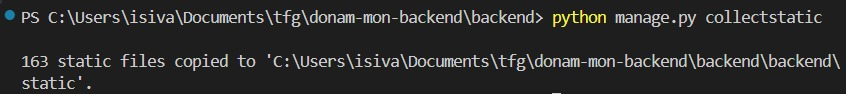
\includegraphics[width=0.9\textwidth]{figs/back.jpg}
    \caption{Recopilación de archivos estáticos con \texttt{collectstatic} en Django}
\end{figure}

\subsection{Gestión de geolocalización y decisión sobre campos GIS}

Aunque el proyecto tiene incluida la librería \texttt{djangorestframework-gis} (puedes verla en el archivo \texttt{requirements.txt}), en realidad no se está usando porque no se han definido campos GIS como \texttt{PointField} o \texttt{PolygonField}, ni tampoco se utiliza el backend geoespacial de Django (\texttt{django.contrib.gis.db.backends.postgis}).

Para la geolocalización, simplemente se guardan las coordenadas de latitud y longitud como campos \texttt{FloatField} en el modelo \texttt{Lugar}:

\begin{lstlisting}[language=Python, caption={Fragmento del modelo Lugar}]
class Lugar(models.Model):
    nombre = models.CharField(max_length=100)
    descripcion = models.TextField()
    latitud = models.FloatField(blank=True, null=True)
    longitud = models.FloatField(blank=True, null=True)
    # ...otros campos...
\end{lstlisting}

Esta solución es suficiente para lo que necesita la aplicación ahora mismo: permite guardar y consultar posiciones geográficas sin complicaciones y sin depender de librerías adicionales ni configuraciones avanzadas. Además, facilita la integración y el despliegue usando el backend estándar de PostgreSQL (\texttt{django.db.backends.postgresql}), sin tener que recurrir a PostGIS.

\textbf{Ventajas de este enfoque:}
\begin{itemize}
    \item El modelo de datos es más sencillo y fácil de mantener.
    \item La integración y el despliegue funcionan en cualquier entorno PostgreSQL, sin requisitos especiales.
    \item Se evitan dependencias y configuraciones extra.
\end{itemize}

En una posible evolución, si en algún momento se necesitan consultas espaciales más avanzadas o funcionalidades GIS (por ejemplo, búsquedas por proximidad o rutas optimizadas), se podría migrar a campos GIS y aprovechar tanto PostGIS como \mbox{\texttt{djangorestframework-gis}} sin demasiada dificultad.
\chapter{Conclusiones}
% !TEX root = ../ejemplo-memoria.tex
% Contenidos del capítulo.
% Las secciones presentadas son orientativas y no representan
% necesariamente la organización que debe tener este capítulo.

\section{Revisión de costes}

\section{Conclusiones}

\section{Trabajo futuro}




\pagestyle{appendix}

\appendix
\chapter{Apéndice}
% !TEX root = ../ejemplo-memoria.tex
\section{Ejemplos del lenguaje de marcado Latex}
\label{cap:apendice}



% Para un nuevo párrafo, basta con dejar una línea en blanco
% No debe utilizarse la doble contrabarra, \\, para nuevos párrafos
Antes de empezar a escribir la memoria debes leerte, al menos, los
dos primeros capítulos del clásico de Tobias
Oeitker~\cite{notsoshort}\footnotemark.

\footnotetext{La última versión puede encontrarse
en~\url{http://tobi.oetiker.ch/lshort/lshort.pdf}.}

El Apéndice~\ref{cap:apendice} recoge algunos ejemplos de edición
con \LaTeX{}.

Ths document is an example of BibTeX using in bibliography management. Three items
are cited: \textit{The \LaTeX\ Companion} book \cite{latexcompanion}, the Einstein
journal paper \cite{einstein}, and the Donald Knuth's website \cite{knuthwebsite}.
The \LaTeX\ related items are \cite{latexcompanion,knuthwebsite}\footnote{Esto está tomado de
\url{https://www.overleaf.com/learn/latex/Bibliography_management_with_bibtex}}.


  \textbf{Texto} en el párrafo 1.

  \textit{Texto} en el párrafo 2.

  \texttt{Texto} en el párrafo 3.


  \begin{itemize}
  \item Consideración 1
  \item Consideración 2
  \end{itemize}

  % Espacio vertical
  \vspace{0.5cm}

  \begin{enumerate}
  \item Punto 1
  \item Punto 2
  \end{enumerate}

A continuación se muestra una ecuación:

  \[ \int_{0}^{1}\frac{1}{x^2+1} dx \]

  Podemos incluir imágenes en formato: png, pdf o jpg.

  En la figura~\ref{fig:diagrama} se muestra un diagrama realizado con \href{yed}{https://www.yworks.com/products/yed}:

  \begin{figure}[!htb]
    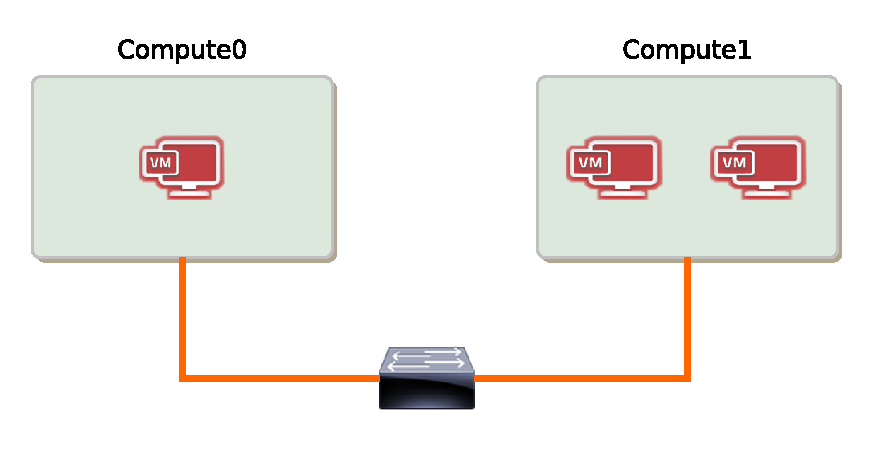
\includegraphics[width=0.8\textwidth]{diagrama.pdf}
    \caption{Esta es una figura que latex decide donde colocar (floating) en el documento.}
    \label{fig:diagrama}
    \end{figure}

  \begin{tabular}{cc}
    Imagen 1 & Imagen 2 \\[2mm]
    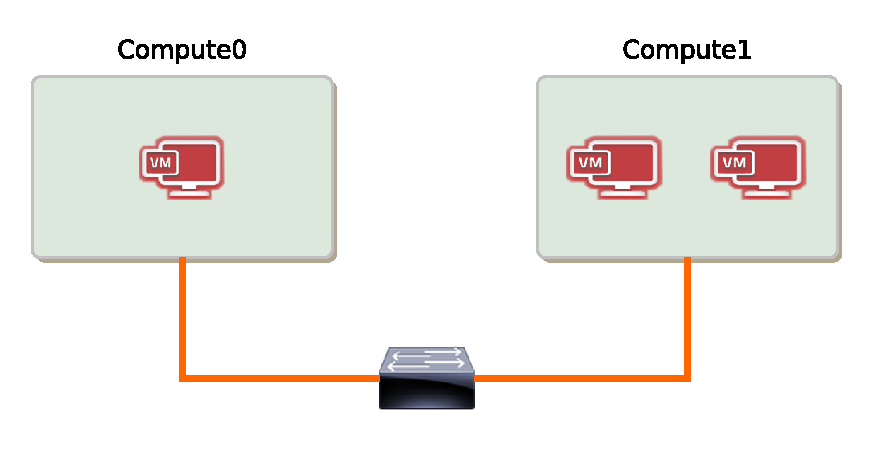
\includegraphics[width=0.4\textwidth]{diagrama.pdf} &  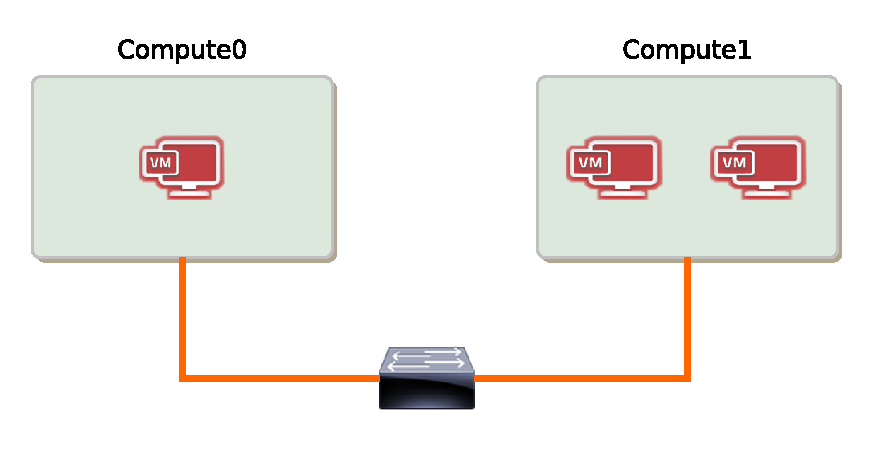
\includegraphics[width=0.4\textwidth]{diagrama.pdf}
  \end{tabular}

  Este es un ejemplo de una tabla:

  \begin{tabular}{|l|c|}
    \hline
    Columna 1 & Columna 2 \\ \hline
    1 & 2 \\ \hline
  \end{tabular}


  \vspace*{1cm}
  O la misma tabla centrada:

  \begin{center}
    \begin{tabular}{|l|c|}
      \hline
      Columna 1 & Columna 2 \\ \hline
      1 & 2 \\ \hline
    \end{tabular}
  \end{center}

  Para generar el fichero PDF:

  \begin{lstlisting}{language=bash}
    pdflatex ejemplo-memoria.tex
    bibtex ejemplo-memoria
    pdflatex ejemplo-memoria.tex
\end{lstlisting}

  También se puede usar \texttt{latexmk} que automáticamente regenera la bibliografía.
  \begin{lstlisting}{language=bash}
    latexmk -pdf ejemplo-memoria.tex
\end{lstlisting}



\addcontentsline{toc}{chapter}{Bibliografía}
\bibliographystyle{unsrt}
\bibliography{bib/bibliografia}




\end{document}

%%% Local Variables:
%%% mode: latex
%%% TeX-master: t
%%% End:
